\input{Carta3.tex}

\renewcommand{\partes}{No por favor}
\renewcommand{\titulodoc}{ENCOVI 2014 - Principales resultados}



\newcommand{\ra}[1]{\renewcommand{\arraystretch}{#1}}
\begin{document}
	\includepdf{portada.pdf}
	\newpage
	\pagestyle{soloarriba}
\clearpage

$\ $
\vspace{14.5cm}

\noindent\begin{tabular}{p{0.9cm}p{6.8cm}}
& 2015.$\,$ Guatemala, Centro América \\
&\Bold Instituto Nacional de Estadística\\[-0.4cm]
&\color{blue!50!black}\url{www.ine.gob.gt}\\[0.9cm]
\end{tabular}\\
\noindent\begin{tabular}{p{0.9cm}p{6.8cm}}
& Está permitida la reproducción parcial o total de los contenidos de este documento con la mención de la fuente. \\[0.5cm]
 
& Este documento fue elaborado empleando  {\Sans R}, Inkscape y {\Logos \XeLaTeX}.\\
\end{tabular} 


\clearpage



	
	\clearpage
	\newpage $\ $

$\ $
\vspace{0.0cm}

\begin{center}
	{\Bold \LARGE AUTORIDADES}\\[1cm]
	
	
	{\Bold \large \color{color1!89!black} JUNTA  DIRECTIVA} \\[0.4cm]
	
	{ \Bold Ministerio de Economía}          \\
	Titular: Sergio de la Torre Gimeno   \\
	Suplente: Jacobo Rey Sigfrido Lee Leiva  \\ [0.4cm]
	
	{\Bold Ministerio de Finanzas} \\
	Titular: Dorval José Carías Samayoa \\
	Suplente: Edwin Oswaldo Martínez Cameros\\[0.4cm]
	
	{\Bold Ministerio de Agricultura, Ganadería y Alimentación} \\
	Titular: José Sebastian Marcucci Ruíz   \\
	Suplente: Henry Giovanni Vásquez Kilkan \\ [0.4cm]
	
	{\Bold Ministerio de Energía y Minas}\\
	Titular: José Miguel de la Vega \\
	Suplente: No hay representante\\ [0.4cm]
	{\Bold Secretaría de Planificación y Programación de la Presidencia}   \\
	Titular: Ekaterina Arbolievna Parrilla Artuguina   \\
	Suplente: Dora Marina Coc Yup\\ [0.4cm]
	{\Bold Banco de Guatemala} \\
	Titular: Julio Roberto Suárez Guerra \\
	Suplente: Sergio Francisco Recinos Rivera\\ [0.4cm]
	{\Bold Universidad de San Carlos de Guatemala de Guatemala} \\
	Titular: Murphy Olimpo Paiz Recinos   \\
	Suplente: Oscar René Paniagua Carrera  \\ [0.4cm]
	{\Bold Universidades Privadas} \\
	Titular: Miguel Ángel Franco de León \\             Suplente: Ariel Rivera Irías\\ [0.4cm]
	{\Bold Comité Coordinador de \ Asociaciones  Agrícolas, Comerciales,Industriales y Financieras} \\
	Titular: Juan Raúl Aguilar Kaehler \\
	Suplente:  Oscar Augusto Sequeira García  \\ [0.4cm]
	
	{\Bold \large \color{color1!89!black} GERENCIA}\\[0.2cm]
	Gerente:  Rubén Darío Narciso Cruz        \\
	Subgerente Técnico:  Jaime Roberto Mejía Salguero\\
	Subgerente Administrativo Financiero:  Orlando Roberto Monzón Girón\\
\end{center}
\clearpage

$\ $
\vspace{1cm}

\begin{center}
	{\Bold \LARGE EQUIPO RESPONSABLE}\\[2cm]
	
	{\Bold \large \color{color1!89!black} REVISIÓN GENERAL}\\[0.2cm]
	Rubén Darío Narciso Cruz\\[0.8cm]
	
	
	{\Bold \large \color{color1!89!black} EQUIPO TÉCNICO}\\[0.2cm]
	Jaime Mejía\\
	Carlos Mancia\\
	Carlos Ortiz\\
	Marvin Reyes\\
	Hugo Rivas\\
	Nelson Santacruz \\
	Luis Fernando Bonilla\\
	Pamela Escobar\\
	Vivian Guzmán\\
	Fabiola Ramírez \\
	Hugo García \\
	Mynor Flores \\[0.8cm]
	
{\Bold \large \color{color1!89!black} DIAGRAMACIÓN Y DISEÑO}\\[0.2cm]
Ligia Morales\\
José Carlos Bonilla Aldana
\end{center}
\vfill
\hrule 
El Instituto Nacional de Estadística agradece el apoyo técnico brindado por el Banco Mundial para la realización de esta encuesta; en especial a Carlos Sobrado,Mario Navarrete y  Elizaveta Perova por su valiosa contribución. 
\cleardoublepage
$\ $\\[2cm]
\noindent {\Bold \huge Presentación}

Aquí va la presentación
\cleardoublepage


	\tableofcontents
	\pagestyle{estandar}
	\setcounter{page}{0}
	




%\INEchaptercarta{Pobreza}{}


\cajita{Línea de pobreza total}{La línea de pobreza extrema representa el costo de adquirir la cantidad mínima de calorías recomendadas.  La línea de pobreza total incluye, además del costo alimenticio, un monto adicional que corresponde al porcentaje de consumo no alimenticio de las personas cuyo consumo de alimentos se encuentra alrededor de la línea de pobreza extrema. }{Línea de pobreza total}{República de Guatemala, serie histórica por Encovi,  en quetzales corrientes}{\ \\[0mm]\begin{tikzpicture}[x=1pt,y=1pt]  % Created by tikzDevice version 0.9 on 2015-11-26 21:52:51
% !TEX encoding = UTF-8 Unicode
\definecolor{fillColor}{RGB}{255,255,255}
\path[use as bounding box,fill=fillColor,fill opacity=0.00] (0,0) rectangle (289.08,198.74);
\begin{scope}
\path[clip] (  0.00,  0.00) rectangle (289.08,198.74);

\path[] (  0.00,  0.00) rectangle (289.08,198.74);
\end{scope}
\begin{scope}
\path[clip] (  0.00,  0.00) rectangle (289.08,198.74);

\path[] ( 13.16, 17.78) rectangle (280.54,191.48);

\path[] ( 13.16, 40.12) --
	(280.54, 40.12);

\path[] ( 13.16, 84.11) --
	(280.54, 84.11);

\path[] ( 13.16,128.11) --
	(280.54,128.11);

\path[] ( 13.16,172.10) --
	(280.54,172.10);

\path[] ( 13.16, 18.12) --
	(280.54, 18.12);

\path[] ( 13.16, 62.11) --
	(280.54, 62.11);

\path[] ( 13.16,106.11) --
	(280.54,106.11);

\path[] ( 13.16,150.11) --
	(280.54,150.11);

\path[] ( 51.36, 17.78) --
	( 51.36,191.48);

\path[] (115.02, 17.78) --
	(115.02,191.48);

\path[] (178.68, 17.78) --
	(178.68,191.48);

\path[] (242.35, 17.78) --
	(242.35,191.48);
\definecolor{drawColor}{RGB}{0,0,255}

\path[draw=drawColor,line width= 1.7pt,line join=round] ( 51.36,125.44) --
	(115.02,158.52) --
	(178.68,183.59) --
	(242.35, 62.11);
\definecolor{drawColor}{RGB}{0,0,0}

\node[text=drawColor,anchor=base,inner sep=0pt, outer sep=0pt, scale=  1.01] at ( 51.36,113.57) {4,318};

\node[text=drawColor,anchor=base east,inner sep=0pt, outer sep=0pt, scale=  1.01] at (111.02,158.52) {6,574};

\node[text=drawColor,anchor=base,inner sep=0pt, outer sep=0pt, scale=  1.01] at (178.68,187.54) {8,283};

\node[text=drawColor,anchor=base,inner sep=0pt, outer sep=0pt, scale=  1.01] at (242.35, 50.24) {0};

\path[draw=drawColor,line width= 0.1pt,line join=round] ( 13.16, 25.67) -- (280.54, 25.67);

\path[] ( 13.16, 17.78) rectangle (280.54,191.48);
\end{scope}
\begin{scope}
\path[clip] (  0.00,  0.00) rectangle (289.08,198.74);

\path[] ( 13.16, 17.78) --
	( 13.16,191.48);
\end{scope}
\begin{scope}
\path[clip] (  0.00,  0.00) rectangle (289.08,198.74);
\definecolor{drawColor}{RGB}{255,255,255}

\node[text=drawColor,text opacity=0.00,anchor=base east,inner sep=0pt, outer sep=0pt, scale=  1.00] at (  6.05, 14.21) {-3000};

\node[text=drawColor,text opacity=0.00,anchor=base east,inner sep=0pt, outer sep=0pt, scale=  1.00] at (  6.05, 58.20) {0};

\node[text=drawColor,text opacity=0.00,anchor=base east,inner sep=0pt, outer sep=0pt, scale=  1.00] at (  6.05,102.20) {3000};

\node[text=drawColor,text opacity=0.00,anchor=base east,inner sep=0pt, outer sep=0pt, scale=  1.00] at (  6.05,146.20) {6000};
\end{scope}
\begin{scope}
\path[clip] (  0.00,  0.00) rectangle (289.08,198.74);

\path[] (  8.89, 18.12) --
	( 13.16, 18.12);

\path[] (  8.89, 62.11) --
	( 13.16, 62.11);

\path[] (  8.89,106.11) --
	( 13.16,106.11);

\path[] (  8.89,150.11) --
	( 13.16,150.11);
\end{scope}
\begin{scope}
\path[clip] (  0.00,  0.00) rectangle (289.08,198.74);

\path[] ( 13.16, 17.78) --
	(280.54, 17.78);
\end{scope}
\begin{scope}
\path[clip] (  0.00,  0.00) rectangle (289.08,198.74);

\path[] ( 51.36, 13.51) --
	( 51.36, 17.78);

\path[] (115.02, 13.51) --
	(115.02, 17.78);

\path[] (178.68, 13.51) --
	(178.68, 17.78);

\path[] (242.35, 13.51) --
	(242.35, 17.78);
\end{scope}
\begin{scope}
\path[clip] (  0.00,  0.00) rectangle (289.08,198.74);
\definecolor{drawColor}{RGB}{0,0,0}

\node[text=drawColor,anchor=base,inner sep=0pt, outer sep=0pt, scale=  1.00] at ( 51.36,  2.85) {2000};

\node[text=drawColor,anchor=base,inner sep=0pt, outer sep=0pt, scale=  1.00] at (115.02,  2.85) {2006};

\node[text=drawColor,anchor=base,inner sep=0pt, outer sep=0pt, scale=  1.00] at (178.68,  2.85) {2011};

\node[text=drawColor,anchor=base,inner sep=0pt, outer sep=0pt, scale=  1.00] at (242.35,  2.85) {2014};
\end{scope}
  \end{tikzpicture}}{Instituto Nacional de Estadística}


\cajita{Pobreza total}{\footnote{$FGT(\alpha)=$
		
		$ \frac{1}{N}\sum_{i=1}^N \left(1-\frac{x_i}{LPT}\right)^\alpha (x_i<LPT) $\\
		
		Con $\alpha=0$}  Para 2014, el \% de la población se encontraba por debajo de la línea de pobreza total y el \% no lograba cubrir el costo del consumo mínimo de alimentos. Se puede observar en la gráfica  que entre 2000 y 2014, la pobreza extrema se redujo / aumentó en x puntos porcentuales, pasando de 15.7\% en 2000 a \% en 2014, mientras que la pobreza total de 56.4\% a \%.  }{Incidencia de pobreza total }{República de Guatemala, serie histórica por Encovi,  en porcentaje}{\ \\[0mm]\begin{tikzpicture}[x=1pt,y=1pt]  % Created by tikzDevice version 0.7.0 on 2015-11-27 12:24:54
% !TEX encoding = UTF-8 Unicode
\definecolor[named]{fillColor}{rgb}{1.00,1.00,1.00}
\path[use as bounding box,fill=fillColor,fill opacity=0.00] (0,0) rectangle (289.08,198.74);
\begin{scope}
\path[clip] (  0.00,  0.00) rectangle (289.08,198.74);

\path[] (  0.00,  0.00) rectangle (289.08,198.74);
\end{scope}
\begin{scope}
\path[clip] (  0.00,  0.00) rectangle (289.08,198.74);

\path[] (  1.64, 17.78) rectangle (280.54,191.48);

\path[] (  1.64, 44.03) --
	(280.54, 44.03);

\path[] (  1.64, 80.76) --
	(280.54, 80.76);

\path[] (  1.64,117.48) --
	(280.54,117.48);

\path[] (  1.64,154.21) --
	(280.54,154.21);

\path[] (  1.64,190.93) --
	(280.54,190.93);

\path[] (  1.64, 25.67) --
	(280.54, 25.67);

\path[] (  1.64, 62.40) --
	(280.54, 62.40);

\path[] (  1.64, 99.12) --
	(280.54, 99.12);

\path[] (  1.64,135.85) --
	(280.54,135.85);

\path[] (  1.64,172.57) --
	(280.54,172.57);

\path[] ( 53.94, 17.78) --
	( 53.94,191.48);

\path[] (141.09, 17.78) --
	(141.09,191.48);

\path[] (228.25, 17.78) --
	(228.25,191.48);
\definecolor[named]{drawColor}{rgb}{0.00,0.00,1.00}

\path[draw=drawColor,line width= 1.7pt,line join=round] ( 53.94,159.39) --
	(141.09,140.09) --
	(228.25,169.94);
\definecolor[named]{drawColor}{rgb}{0.00,0.00,0.00}

\node[text=drawColor,anchor=base,inner sep=0pt, outer sep=0pt, scale=  1.01] at ( 53.94,163.34) {56.4};

\node[text=drawColor,anchor=base,inner sep=0pt, outer sep=0pt, scale=  1.01] at (141.09,128.22) {51.2};

\node[text=drawColor,anchor=base,inner sep=0pt, outer sep=0pt, scale=  1.01] at (228.25,173.90) {59.3};
\definecolor[named]{fillColor}{rgb}{0.00,0.00,0.00}

\path[draw=drawColor,line width= 0.1pt,line join=round,fill=fillColor] (  1.64, 25.67) -- (280.54, 25.67);

\path[] (  1.64, 17.78) rectangle (280.54,191.48);
\end{scope}
\begin{scope}
\path[clip] (  0.00,  0.00) rectangle (289.08,198.74);

\path[] (  1.64, 17.78) --
	(  1.64,191.48);
\end{scope}
\begin{scope}
\path[clip] (  0.00,  0.00) rectangle (289.08,198.74);

\path[] (  0.00, 25.67) --
	(  1.64, 25.67);

\path[] (  0.00, 62.40) --
	(  1.64, 62.40);

\path[] (  0.00, 99.12) --
	(  1.64, 99.12);

\path[] (  0.00,135.85) --
	(  1.64,135.85);

\path[] (  0.00,172.57) --
	(  1.64,172.57);
\end{scope}
\begin{scope}
\path[clip] (  0.00,  0.00) rectangle (289.08,198.74);

\path[] (  1.64, 17.78) --
	(280.54, 17.78);
\end{scope}
\begin{scope}
\path[clip] (  0.00,  0.00) rectangle (289.08,198.74);

\path[] ( 53.94, 13.51) --
	( 53.94, 17.78);

\path[] (141.09, 13.51) --
	(141.09, 17.78);

\path[] (228.25, 13.51) --
	(228.25, 17.78);
\end{scope}
\begin{scope}
\path[clip] (  0.00,  0.00) rectangle (289.08,198.74);
\definecolor[named]{drawColor}{rgb}{0.00,0.00,0.00}

\node[text=drawColor,anchor=base,inner sep=0pt, outer sep=0pt, scale=  1.00] at ( 53.94,  2.85) {2000};

\node[text=drawColor,anchor=base,inner sep=0pt, outer sep=0pt, scale=  1.00] at (141.09,  2.85) {2006};

\node[text=drawColor,anchor=base,inner sep=0pt, outer sep=0pt, scale=  1.00] at (228.25,  2.85) {2014};
\end{scope}
  \end{tikzpicture}}{Instituto Nacional de Estadística}


\cajita{Pobreza total por área de residencia}{\textollamada{Para el año 2014, el X\% de la población habitaba en áreas urbanas y el y\% en áreas rurales.} Al desagregar por las distintas características de la población, se observan amplias brechas entre los distintos grupos de población. En general, los mayores niveles de pobreza se observan en la población indígena y la población que habita en áreas rurales. Aunque la pobreza se ha reducido para estos dos grupos de población en el período estudiado, las diferencias todavía son amplias con relación a la población no indígena y a la población que habita  en áreas urbanas, respectivamente. }{Incidencia de pobreza total por área de residencia}{República de Guatemala, serie histórica por Encovi,  en porcentaje}{\ \\[0mm]\begin{tikzpicture}[x=1pt,y=1pt]  % Created by tikzDevice version 0.9 on 2015-11-26 22:20:33
% !TEX encoding = UTF-8 Unicode
\definecolor{fillColor}{RGB}{255,255,255}
\path[use as bounding box,fill=fillColor,fill opacity=0.00] (0,0) rectangle (289.08,198.74);
\begin{scope}
\path[clip] (  0.00,  0.00) rectangle (289.08,198.74);

\path[] (  0.00,  0.00) rectangle (289.08,198.74);
\end{scope}
\begin{scope}
\path[clip] (  0.00,  0.00) rectangle (289.08,198.74);

\path[] (  7.11, 20.62) rectangle (289.08,171.35);

\path[] ( 59.98, 20.62) --
	( 59.98,171.35);

\path[] (148.10, 20.62) --
	(148.10,171.35);

\path[] (236.21, 20.62) --
	(236.21,171.35);
\definecolor{drawColor}{RGB}{0,0,255}
\definecolor{fillColor}{RGB}{0,0,255}

\path[draw=drawColor,line width= 0.6pt,line join=round,fill=fillColor] ( 22.53, 20.62) rectangle ( 57.78,167.65);
\definecolor{drawColor}{RGB}{157,187,255}
\definecolor{fillColor}{RGB}{157,187,255}

\path[draw=drawColor,line width= 0.6pt,line join=round,fill=fillColor] ( 62.18, 20.62) rectangle ( 97.43,100.33);
\definecolor{drawColor}{RGB}{0,0,255}
\definecolor{fillColor}{RGB}{0,0,255}

\path[draw=drawColor,line width= 0.6pt,line join=round,fill=fillColor] (110.65, 20.62) rectangle (145.89,163.29);
\definecolor{drawColor}{RGB}{157,187,255}
\definecolor{fillColor}{RGB}{157,187,255}

\path[draw=drawColor,line width= 0.6pt,line join=round,fill=fillColor] (150.30, 20.62) rectangle (185.55, 89.73);
\definecolor{drawColor}{RGB}{0,0,255}
\definecolor{fillColor}{RGB}{0,0,255}

\path[draw=drawColor,line width= 0.6pt,line join=round,fill=fillColor] (198.76, 20.62) rectangle (234.01,171.35);
\definecolor{drawColor}{RGB}{157,187,255}
\definecolor{fillColor}{RGB}{157,187,255}

\path[draw=drawColor,line width= 0.6pt,line join=round,fill=fillColor] (238.41, 20.62) rectangle (273.66,109.22);
\definecolor{drawColor}{RGB}{0,0,0}

\path[draw=drawColor,line width= 0.6pt,line join=round] (  7.11, 20.62) -- (289.08, 20.62);

\node[text=drawColor,anchor=base,inner sep=0pt, outer sep=0pt, scale=  0.82] at ( 40.16,170.87) {77.3};

\node[text=drawColor,anchor=base,inner sep=0pt, outer sep=0pt, scale=  0.82] at ( 79.81,103.56) {41.9};

\node[text=drawColor,anchor=base,inner sep=0pt, outer sep=0pt, scale=  0.82] at (128.27,166.51) {75.0};

\node[text=drawColor,anchor=base,inner sep=0pt, outer sep=0pt, scale=  0.82] at (167.92, 92.96) {36.3};

\node[text=drawColor,anchor=base,inner sep=0pt, outer sep=0pt, scale=  0.82] at (216.39,174.57) {79.2};

\node[text=drawColor,anchor=base,inner sep=0pt, outer sep=0pt, scale=  0.82] at (256.04,112.45) {46.6};

\path[] (  7.11, 20.62) rectangle (289.08,171.35);
\end{scope}
\begin{scope}
\path[clip] (  0.00,  0.00) rectangle (289.08,198.74);

\path[] (  7.11, 20.62) --
	(  7.11,171.35);
\end{scope}
\begin{scope}
\path[clip] (  0.00,  0.00) rectangle (289.08,198.74);

\path[] (  7.11, 20.62) --
	(289.08, 20.62);
\end{scope}
\begin{scope}
\path[clip] (  0.00,  0.00) rectangle (289.08,198.74);

\path[] ( 59.98, 16.35) --
	( 59.98, 20.62);

\path[] (148.10, 16.35) --
	(148.10, 20.62);

\path[] (236.21, 16.35) --
	(236.21, 20.62);
\end{scope}
\begin{scope}
\path[clip] (  0.00,  0.00) rectangle (289.08,198.74);
\definecolor{drawColor}{RGB}{0,0,0}

\node[text=drawColor,anchor=base,inner sep=0pt, outer sep=0pt, scale=  1.00] at ( 59.98,  5.69) {2000};

\node[text=drawColor,anchor=base,inner sep=0pt, outer sep=0pt, scale=  1.00] at (148.10,  5.69) {2006};

\node[text=drawColor,anchor=base,inner sep=0pt, outer sep=0pt, scale=  1.00] at (236.21,  5.69) {2014};
\end{scope}
\begin{scope}
\path[clip] (  0.00,  0.00) rectangle (289.08,198.74);
\coordinate (apoyo) at (54.15,187.71);
\coordinate (longitudFicticia) at (7.11,11.03);
\coordinate (longitud) at (7.11,7.11);
\coordinate (desX) at (133.24,0);
\coordinate (desY) at (0,1.96);
\definecolor[named]{ct1}{HTML}{
0000FF
}
\definecolor[named]{ct2}{HTML}{
9DBBFF
}
\definecolor[named]{ctb1}{HTML}{
0000FF
}
\definecolor[named]{ctb2}{HTML}{
9DBBFF
}
\path [fill=none] (apoyo) rectangle ($(apoyo)+(longitudFicticia)$)
node [xshift=0.3cm,inner sep=0pt, outer sep=0pt,midway,right,scale = 0.9]{Indígena};
\draw [color = ctb1,fill=ct1] ( $(apoyo)  + (desY) $) rectangle ($(apoyo)+ (desY) +(longitud)$);
\path [fill=none] ($(apoyo)+(desX)$) rectangle ($(apoyo)+(desX)+(longitudFicticia)$)
node [xshift=0.3cm,inner sep=0pt, outer sep=0pt,midway,right,scale = 0.9]{No indígena};
\draw [color = ctb2 ,fill=ct2] ( $(apoyo)  + (desY) + (desX) $) rectangle ($(apoyo)+ (desY)+ (desX) +(longitud)$);
\end{scope}
  \end{tikzpicture}}{Instituto Nacional de Estadística}


\cajita{Pobreza total por etnicidad}{\textollamada{Para el año 2014, el X\% de la población se autoidentificó como perteneciente a un pueblo indígena.} Al desagregar por las distintas características de la población, se observan amplias brechas entre los distintos grupos de población. En general, los mayores niveles de pobreza se observan en la población indígena y la población que habita en áreas rurales. Aunque la pobreza se ha reducido para estos dos grupos de población en el período estudiado, las diferencias todavía son amplias con relación a la población no indígena y a la población que habita  en áreas urbanas, respectivamente.}{Incidencia de pobreza total por etnicidad}{República de Guatemala, serie histórica por Encovi,  en porcentaje}{\ \\[0mm]\begin{tikzpicture}[x=1pt,y=1pt]  \input{graficas/1_04.tex}  \end{tikzpicture}}{Instituto Nacional de Estadística}


\cajota{Pobreza total en los departamentos}{En el mapa se observa que los departamentos con mayores niveles de pobreza }{Incidencia de pobreza total}{Por departamento, año 2014, en porcentaje}{\includegraphics[width=52\cuadri]{graficas/1_05.pdf}}{Instituto Nacional de Estadística}


\cajita{Línea de pobreza extrema}{\textollamada{Para el año 2014, la cantidad de calorías mínimas recomendadas por persona al día era de. } La línea de pobreza extrema representa el costo de adquirir la cantidad mínima de calorías recomendadas.  La línea de pobreza total incluye, además del costo alimenticio, un monto adicional que corresponde al porcentaje de consumo no alimenticio de las personas cuyo consumo de alimentos se encuentra alrededor de la línea de pobreza extrema. }{Línea de pobreza extrema}{República de Guatemala, serie histórica por Encovi, en quetzales corrientes}{\ \\[0mm]\begin{tikzpicture}[x=1pt,y=1pt]  % Created by tikzDevice version 0.7.0 on 2015-08-07 17:47:05
% !TEX encoding = UTF-8 Unicode
\definecolor[named]{fillColor}{rgb}{1.00,1.00,1.00}
\path[use as bounding box,fill=fillColor,fill opacity=0.00] (0,0) rectangle (289.08,198.74);
\begin{scope}
\path[clip] (  0.00,  0.00) rectangle (289.08,198.74);
\definecolor[named]{drawColor}{rgb}{1.00,1.00,1.00}

\path[draw=drawColor,line width= 0.6pt,line join=round,line cap=round] (  0.00,  0.00) rectangle (289.08,198.74);
\end{scope}
\begin{scope}
\path[clip] (  0.00,  0.00) rectangle (289.08,198.74);

\path[] ( 10.40, 17.78) rectangle (280.54,191.48);

\path[] ( 10.40, 34.38) --
	(280.54, 34.38);

\path[] ( 10.40, 89.85) --
	(280.54, 89.85);

\path[] ( 10.40,145.31) --
	(280.54,145.31);

\path[] ( 10.40, 62.11) --
	(280.54, 62.11);

\path[] ( 10.40,117.58) --
	(280.54,117.58);

\path[] ( 10.40,173.05) --
	(280.54,173.05);

\path[] ( 48.99, 17.78) --
	( 48.99,191.48);

\path[] (113.31, 17.78) --
	(113.31,191.48);

\path[] (177.63, 17.78) --
	(177.63,191.48);

\path[] (241.95, 17.78) --
	(241.95,191.48);
\definecolor[named]{drawColor}{rgb}{0.00,0.00,1.00}

\path[draw=drawColor,line width= 1.7pt,line join=round] ( 48.99,115.11) --
	(113.31,151.03) --
	(177.63,183.59) --
	(241.95, 62.11);
\definecolor[named]{drawColor}{rgb}{0.00,0.00,0.00}

\node[text=drawColor,anchor=base,inner sep=0pt, outer sep=0pt, scale=  0.95] at ( 48.99,103.93) {1,911};

\node[text=drawColor,anchor=base east,inner sep=0pt, outer sep=0pt, scale=  0.95] at (109.54,151.03) {3,206};

\node[text=drawColor,anchor=base,inner sep=0pt, outer sep=0pt, scale=  0.95] at (177.63,187.31) {4,380};

\node[text=drawColor,anchor=base,inner sep=0pt, outer sep=0pt, scale=  0.95] at (241.95, 50.93) {0};
\definecolor[named]{fillColor}{rgb}{0.00,0.00,0.00}

\path[draw=drawColor,line width= 0.1pt,line join=round,fill=fillColor] ( 10.40, 25.67) -- (280.54, 25.67);
\end{scope}
\begin{scope}
\path[clip] (  0.00,  0.00) rectangle (289.08,198.74);

\path[] ( 10.40, 17.78) --
	( 10.40,191.48);
\end{scope}
\begin{scope}
\path[clip] (  0.00,  0.00) rectangle (289.08,198.74);
\definecolor[named]{drawColor}{rgb}{1.00,1.00,1.00}

\node[text=drawColor,text opacity=0.00,anchor=base east,inner sep=0pt, outer sep=0pt, scale=  1.00] at (  3.29, 58.20) {0};

\node[text=drawColor,text opacity=0.00,anchor=base east,inner sep=0pt, outer sep=0pt, scale=  1.00] at (  3.29,113.67) {2000};

\node[text=drawColor,text opacity=0.00,anchor=base east,inner sep=0pt, outer sep=0pt, scale=  1.00] at (  3.29,169.14) {4000};
\end{scope}
\begin{scope}
\path[clip] (  0.00,  0.00) rectangle (289.08,198.74);

\path[] (  6.13, 62.11) --
	( 10.40, 62.11);

\path[] (  6.13,117.58) --
	( 10.40,117.58);

\path[] (  6.13,173.05) --
	( 10.40,173.05);
\end{scope}
\begin{scope}
\path[clip] (  0.00,  0.00) rectangle (289.08,198.74);

\path[] ( 10.40, 17.78) --
	(280.54, 17.78);
\end{scope}
\begin{scope}
\path[clip] (  0.00,  0.00) rectangle (289.08,198.74);

\path[] ( 48.99, 13.51) --
	( 48.99, 17.78);

\path[] (113.31, 13.51) --
	(113.31, 17.78);

\path[] (177.63, 13.51) --
	(177.63, 17.78);

\path[] (241.95, 13.51) --
	(241.95, 17.78);
\end{scope}
\begin{scope}
\path[clip] (  0.00,  0.00) rectangle (289.08,198.74);
\definecolor[named]{drawColor}{rgb}{0.00,0.00,0.00}

\node[text=drawColor,anchor=base,inner sep=0pt, outer sep=0pt, scale=  1.00] at ( 48.99,  2.85) {2000};

\node[text=drawColor,anchor=base,inner sep=0pt, outer sep=0pt, scale=  1.00] at (113.31,  2.85) {2006};

\node[text=drawColor,anchor=base,inner sep=0pt, outer sep=0pt, scale=  1.00] at (177.63,  2.85) {2011};

\node[text=drawColor,anchor=base,inner sep=0pt, outer sep=0pt, scale=  1.00] at (241.95,  2.85) {2014};
\end{scope}
  \end{tikzpicture}}{Instituto Nacional de Estadística}


\cajita{Pobreza extrema}{\footnote{$FGT(\alpha)=$
		
		$ \frac{1}{N}\sum_{i=1}^N \left(1-\frac{x_i}{LPT}\right)^\alpha (x_i<LPT) $\\
		
		Con $\alpha=0$} }{Incidencia de pobreza extrema}{República de Guatemala, serie histórica por Encovi, en porcentaje}{\ \\[0mm]\begin{tikzpicture}[x=1pt,y=1pt]  % Created by tikzDevice version 0.9 on 2015-11-26 21:53:14
% !TEX encoding = UTF-8 Unicode
\definecolor{fillColor}{RGB}{255,255,255}
\path[use as bounding box,fill=fillColor,fill opacity=0.00] (0,0) rectangle (289.08,198.74);
\begin{scope}
\path[clip] (  0.00,  0.00) rectangle (289.08,198.74);

\path[] (  0.00,  0.00) rectangle (289.08,198.74);
\end{scope}
\begin{scope}
\path[clip] (  0.00,  0.00) rectangle (289.08,198.74);

\path[] (  1.64, 17.78) rectangle (280.54,191.48);

\path[] (  1.64, 42.77) --
	(280.54, 42.77);

\path[] (  1.64, 81.46) --
	(280.54, 81.46);

\path[] (  1.64,120.14) --
	(280.54,120.14);

\path[] (  1.64,158.83) --
	(280.54,158.83);

\path[] (  1.64, 23.43) --
	(280.54, 23.43);

\path[] (  1.64, 62.11) --
	(280.54, 62.11);

\path[] (  1.64,100.80) --
	(280.54,100.80);

\path[] (  1.64,139.49) --
	(280.54,139.49);

\path[] (  1.64,178.17) --
	(280.54,178.17);

\path[] ( 41.49, 17.78) --
	( 41.49,191.48);

\path[] (107.89, 17.78) --
	(107.89,191.48);

\path[] (174.30, 17.78) --
	(174.30,191.48);

\path[] (240.70, 17.78) --
	(240.70,191.48);
\definecolor{drawColor}{RGB}{0,0,255}

\path[draw=drawColor,line width= 1.7pt,line join=round] ( 41.49,183.59) --
	(107.89,180.20) --
	(174.30,165.02) --
	(240.70, 62.11);
\definecolor{drawColor}{RGB}{0,0,0}

\node[text=drawColor,anchor=base,inner sep=0pt, outer sep=0pt, scale=  1.01] at ( 41.49,187.54) {15.7};

\node[text=drawColor,anchor=base west,inner sep=0pt, outer sep=0pt, scale=  1.01] at (107.89,184.16) {15.3};

\node[text=drawColor,anchor=base west,inner sep=0pt, outer sep=0pt, scale=  1.01] at (174.30,168.97) {13.3};

\node[text=drawColor,anchor=base,inner sep=0pt, outer sep=0pt, scale=  1.01] at (240.70, 50.24) {0.0};

\path[draw=drawColor,line width= 0.1pt,line join=round] (  1.64, 25.67) -- (280.54, 25.67);

\path[] (  1.64, 17.78) rectangle (280.54,191.48);
\end{scope}
\begin{scope}
\path[clip] (  0.00,  0.00) rectangle (289.08,198.74);

\path[] (  1.64, 17.78) --
	(  1.64,191.48);
\end{scope}
\begin{scope}
\path[clip] (  0.00,  0.00) rectangle (289.08,198.74);

\path[] (  0.00, 23.43) --
	(  1.64, 23.43);

\path[] (  0.00, 62.11) --
	(  1.64, 62.11);

\path[] (  0.00,100.80) --
	(  1.64,100.80);

\path[] (  0.00,139.49) --
	(  1.64,139.49);

\path[] (  0.00,178.17) --
	(  1.64,178.17);
\end{scope}
\begin{scope}
\path[clip] (  0.00,  0.00) rectangle (289.08,198.74);

\path[] (  1.64, 17.78) --
	(280.54, 17.78);
\end{scope}
\begin{scope}
\path[clip] (  0.00,  0.00) rectangle (289.08,198.74);

\path[] ( 41.49, 13.51) --
	( 41.49, 17.78);

\path[] (107.89, 13.51) --
	(107.89, 17.78);

\path[] (174.30, 13.51) --
	(174.30, 17.78);

\path[] (240.70, 13.51) --
	(240.70, 17.78);
\end{scope}
\begin{scope}
\path[clip] (  0.00,  0.00) rectangle (289.08,198.74);
\definecolor{drawColor}{RGB}{0,0,0}

\node[text=drawColor,anchor=base,inner sep=0pt, outer sep=0pt, scale=  1.00] at ( 41.49,  2.85) {2000};

\node[text=drawColor,anchor=base,inner sep=0pt, outer sep=0pt, scale=  1.00] at (107.89,  2.85) {2006};

\node[text=drawColor,anchor=base,inner sep=0pt, outer sep=0pt, scale=  1.00] at (174.30,  2.85) {2011};

\node[text=drawColor,anchor=base,inner sep=0pt, outer sep=0pt, scale=  1.00] at (240.70,  2.85) {2014};
\end{scope}
  \end{tikzpicture}}{Instituto Nacional de Estadística}


\cajita{Pobreza extrema por área de residencia}{\textollamada{Para el año 2014, el X\% de la población habitaba en áreas urbanas y el y\% en áreas rurales.}          }{Incidencia de pobreza extrema por área residencia}{República de Guatemala, serie histórica por Encovi, en porcentaje}{\ \\[0mm]\begin{tikzpicture}[x=1pt,y=1pt]  % Created by tikzDevice version 0.7.0 on 2015-08-07 17:47:05
% !TEX encoding = UTF-8 Unicode
\definecolor[named]{fillColor}{rgb}{1.00,1.00,1.00}
\path[use as bounding box,fill=fillColor,fill opacity=0.00] (0,0) rectangle (289.08,198.74);
\begin{scope}
\path[clip] (  0.00,  0.00) rectangle (289.08,198.74);
\definecolor[named]{drawColor}{rgb}{1.00,1.00,1.00}

\path[draw=drawColor,line width= 0.6pt,line join=round,line cap=round] (  0.00,  0.00) rectangle (289.08,198.74);
\end{scope}
\begin{scope}
\path[clip] (  0.00,  0.00) rectangle (289.08,198.74);

\path[] (  7.11, 20.62) rectangle (289.08,174.77);

\path[] ( 47.39, 20.62) --
	( 47.39,174.77);

\path[] (114.53, 20.62) --
	(114.53,174.77);

\path[] (181.66, 20.62) --
	(181.66,174.77);

\path[] (248.80, 20.62) --
	(248.80,174.77);
\definecolor[named]{drawColor}{rgb}{0.00,0.00,1.00}
\definecolor[named]{fillColor}{rgb}{0.00,0.00,1.00}

\path[draw=drawColor,line width= 0.6pt,line join=round,fill=fillColor] ( 18.86, 20.62) rectangle ( 45.72, 38.49);
\definecolor[named]{drawColor}{rgb}{0.62,0.73,1.00}
\definecolor[named]{fillColor}{rgb}{0.62,0.73,1.00}

\path[draw=drawColor,line width= 0.6pt,line join=round,fill=fillColor] ( 49.07, 20.62) rectangle ( 75.93,170.52);
\definecolor[named]{drawColor}{rgb}{0.00,0.00,1.00}
\definecolor[named]{fillColor}{rgb}{0.00,0.00,1.00}

\path[draw=drawColor,line width= 0.6pt,line join=round,fill=fillColor] ( 86.00, 20.62) rectangle (112.85, 54.27);
\definecolor[named]{drawColor}{rgb}{0.62,0.73,1.00}
\definecolor[named]{fillColor}{rgb}{0.62,0.73,1.00}

\path[draw=drawColor,line width= 0.6pt,line join=round,fill=fillColor] (116.21, 20.62) rectangle (143.06,174.77);
\definecolor[named]{drawColor}{rgb}{0.00,0.00,1.00}
\definecolor[named]{fillColor}{rgb}{0.00,0.00,1.00}

\path[draw=drawColor,line width= 0.6pt,line join=round,fill=fillColor] (153.13, 20.62) rectangle (179.99, 52.58);
\definecolor[named]{drawColor}{rgb}{0.62,0.73,1.00}
\definecolor[named]{fillColor}{rgb}{0.62,0.73,1.00}

\path[draw=drawColor,line width= 0.6pt,line join=round,fill=fillColor] (183.34, 20.62) rectangle (210.20,153.85);
\definecolor[named]{drawColor}{rgb}{0.00,0.00,1.00}
\definecolor[named]{fillColor}{rgb}{0.00,0.00,1.00}

\path[draw=drawColor,line width= 0.6pt,line join=round,fill=fillColor] (220.27, 20.62) rectangle (247.12, 20.62);
\definecolor[named]{drawColor}{rgb}{0.62,0.73,1.00}
\definecolor[named]{fillColor}{rgb}{0.62,0.73,1.00}

\path[draw=drawColor,line width= 0.6pt,line join=round,fill=fillColor] (250.48, 20.62) rectangle (277.33, 20.62);
\definecolor[named]{drawColor}{rgb}{0.00,0.00,0.00}
\definecolor[named]{fillColor}{rgb}{0.00,0.00,0.00}

\path[draw=drawColor,line width= 0.6pt,line join=round,fill=fillColor] (  7.11, 20.62) -- (289.08, 20.62);

\node[text=drawColor,anchor=base,inner sep=0pt, outer sep=0pt, scale=  0.82] at ( 32.29, 41.71) {2.8};

\node[text=drawColor,anchor=base,inner sep=0pt, outer sep=0pt, scale=  0.82] at ( 62.50,173.75) {23.8};

\node[text=drawColor,anchor=base,inner sep=0pt, outer sep=0pt, scale=  0.82] at ( 99.42, 57.49) {5.3};

\node[text=drawColor,anchor=base,inner sep=0pt, outer sep=0pt, scale=  0.82] at (129.63,177.99) {24.4};

\node[text=drawColor,anchor=base,inner sep=0pt, outer sep=0pt, scale=  0.82] at (166.56, 55.80) {5.1};

\node[text=drawColor,anchor=base,inner sep=0pt, outer sep=0pt, scale=  0.82] at (196.77,157.08) {21.1};

\node[text=drawColor,anchor=base,inner sep=0pt, outer sep=0pt, scale=  0.82] at (233.69, 23.84) {0.0};

\node[text=drawColor,anchor=base,inner sep=0pt, outer sep=0pt, scale=  0.82] at (263.90, 23.84) {0.0};
\end{scope}
\begin{scope}
\path[clip] (  0.00,  0.00) rectangle (289.08,198.74);

\path[] (  7.11, 20.62) --
	(  7.11,174.77);
\end{scope}
\begin{scope}
\path[clip] (  0.00,  0.00) rectangle (289.08,198.74);

\path[] (  7.11, 20.62) --
	(289.08, 20.62);
\end{scope}
\begin{scope}
\path[clip] (  0.00,  0.00) rectangle (289.08,198.74);

\path[] ( 47.39, 16.35) --
	( 47.39, 20.62);

\path[] (114.53, 16.35) --
	(114.53, 20.62);

\path[] (181.66, 16.35) --
	(181.66, 20.62);

\path[] (248.80, 16.35) --
	(248.80, 20.62);
\end{scope}
\begin{scope}
\path[clip] (  0.00,  0.00) rectangle (289.08,198.74);
\definecolor[named]{drawColor}{rgb}{0.00,0.00,0.00}

\node[text=drawColor,anchor=base,inner sep=0pt, outer sep=0pt, scale=  1.00] at ( 47.39,  5.69) {2000};

\node[text=drawColor,anchor=base,inner sep=0pt, outer sep=0pt, scale=  1.00] at (114.53,  5.69) {2006};

\node[text=drawColor,anchor=base,inner sep=0pt, outer sep=0pt, scale=  1.00] at (181.66,  5.69) {2011};

\node[text=drawColor,anchor=base,inner sep=0pt, outer sep=0pt, scale=  1.00] at (248.80,  5.69) {2014};
\end{scope}
\coordinate (apoyo) at (57.27,191.13);
\coordinate (longitudFicticia) at (7.11,7.61);
\coordinate (longitud) at (7.11,7.11);
\coordinate (desX) at (142.24,0);
\coordinate (desY) at (0,0.25);
\definecolor[named]{ct1}{HTML}{
0000FF
}
\definecolor[named]{ct2}{HTML}{
9DBBFF
}
\definecolor[named]{ctb1}{HTML}{
0000FF
}
\definecolor[named]{ctb2}{HTML}{
9DBBFF
}
\path [fill=none] (apoyo) rectangle ($(apoyo)+(longitudFicticia)$)
node [xshift=0.3cm,inner sep=0pt, outer sep=0pt,midway,right,scale = 0.9]{Urbana};
\draw [color = ctb1,fill=ct1] ( $(apoyo)  + (desY) $) rectangle ($(apoyo)+ (desY) +(longitud)$);
\path [fill=none] ($(apoyo)+(desX)$) rectangle ($(apoyo)+(desX)+(longitudFicticia)$)
node [xshift=0.3cm,inner sep=0pt, outer sep=0pt,midway,right,scale = 0.9]{Rural};
\draw [color = ctb2 ,fill=ct2] ( $(apoyo)  + (desY) + (desX) $) rectangle ($(apoyo)+ (desY)+ (desX) +(longitud)$);
  \end{tikzpicture}}{Instituto Nacional de Estadística}


\cajita{Pobreza extrema por etnicidad}{0}{\textollamada{Para el año 2014, el X\% de la población se autoidentificó como perteneciente a un pueblo indígena.} Incidencia de pobreza extrema por etnicidad}{República de Guatemala, serie histórica por Encovi,  en porcentaje}{\ \\[0mm]\begin{tikzpicture}[x=1pt,y=1pt]  % Created by tikzDevice version 0.9 on 2015-11-26 21:53:21
% !TEX encoding = UTF-8 Unicode
\definecolor{fillColor}{RGB}{255,255,255}
\path[use as bounding box,fill=fillColor,fill opacity=0.00] (0,0) rectangle (289.08,198.74);
\begin{scope}
\path[clip] (  0.00,  0.00) rectangle (289.08,198.74);

\path[] (  0.00,  0.00) rectangle (289.08,198.74);
\end{scope}
\begin{scope}
\path[clip] (  0.00,  0.00) rectangle (289.08,198.74);

\path[] (  7.11, 20.62) rectangle (289.08,172.42);

\path[] ( 47.39, 20.62) --
	( 47.39,172.42);

\path[] (114.53, 20.62) --
	(114.53,172.42);

\path[] (181.66, 20.62) --
	(181.66,172.42);

\path[] (248.80, 20.62) --
	(248.80,172.42);
\definecolor{drawColor}{RGB}{0,0,255}
\definecolor{fillColor}{RGB}{0,0,255}

\path[draw=drawColor,line width= 0.6pt,line join=round,fill=fillColor] ( 18.86, 20.62) rectangle ( 45.72,171.26);
\definecolor{drawColor}{RGB}{157,187,255}
\definecolor{fillColor}{RGB}{157,187,255}

\path[draw=drawColor,line width= 0.6pt,line join=round,fill=fillColor] ( 49.07, 20.62) rectangle ( 75.93, 64.04);
\definecolor{drawColor}{RGB}{0,0,255}
\definecolor{fillColor}{RGB}{0,0,255}

\path[draw=drawColor,line width= 0.6pt,line join=round,fill=fillColor] ( 86.00, 20.62) rectangle (112.85,172.42);
\definecolor{drawColor}{RGB}{157,187,255}
\definecolor{fillColor}{RGB}{157,187,255}

\path[draw=drawColor,line width= 0.6pt,line join=round,fill=fillColor] (116.21, 20.62) rectangle (143.06, 63.75);
\definecolor{drawColor}{RGB}{0,0,255}
\definecolor{fillColor}{RGB}{0,0,255}

\path[draw=drawColor,line width= 0.6pt,line join=round,fill=fillColor] (153.13, 20.62) rectangle (179.99,144.39);
\definecolor{drawColor}{RGB}{157,187,255}
\definecolor{fillColor}{RGB}{157,187,255}

\path[draw=drawColor,line width= 0.6pt,line join=round,fill=fillColor] (183.34, 20.62) rectangle (210.20, 61.67);
\definecolor{drawColor}{RGB}{0,0,255}
\definecolor{fillColor}{RGB}{0,0,255}

\path[draw=drawColor,line width= 0.6pt,line join=round,fill=fillColor] (220.27, 20.62) rectangle (247.12, 20.62);
\definecolor{drawColor}{RGB}{157,187,255}
\definecolor{fillColor}{RGB}{157,187,255}

\path[draw=drawColor,line width= 0.6pt,line join=round,fill=fillColor] (250.48, 20.62) rectangle (277.33, 20.62);
\definecolor{drawColor}{RGB}{0,0,0}

\path[draw=drawColor,line width= 0.6pt,line join=round] (  7.11, 20.62) -- (289.08, 20.62);

\node[text=drawColor,anchor=base,inner sep=0pt, outer sep=0pt, scale=  0.82] at ( 32.29,174.48) {27.1};

\node[text=drawColor,anchor=base,inner sep=0pt, outer sep=0pt, scale=  0.82] at ( 62.50, 67.26) {7.8};

\node[text=drawColor,anchor=base,inner sep=0pt, outer sep=0pt, scale=  0.82] at ( 99.42,175.65) {27.3};

\node[text=drawColor,anchor=base,inner sep=0pt, outer sep=0pt, scale=  0.82] at (129.63, 66.97) {7.8};

\node[text=drawColor,anchor=base,inner sep=0pt, outer sep=0pt, scale=  0.82] at (166.56,147.62) {22.3};

\node[text=drawColor,anchor=base,inner sep=0pt, outer sep=0pt, scale=  0.82] at (196.77, 64.90) {7.4};

\node[text=drawColor,anchor=base,inner sep=0pt, outer sep=0pt, scale=  0.82] at (233.69, 23.84) {0.0};

\node[text=drawColor,anchor=base,inner sep=0pt, outer sep=0pt, scale=  0.82] at (263.90, 23.84) {0.0};

\path[] (  7.11, 20.62) rectangle (289.08,172.42);
\end{scope}
\begin{scope}
\path[clip] (  0.00,  0.00) rectangle (289.08,198.74);

\path[] (  7.11, 20.62) --
	(  7.11,172.42);
\end{scope}
\begin{scope}
\path[clip] (  0.00,  0.00) rectangle (289.08,198.74);

\path[] (  7.11, 20.62) --
	(289.08, 20.62);
\end{scope}
\begin{scope}
\path[clip] (  0.00,  0.00) rectangle (289.08,198.74);

\path[] ( 47.39, 16.35) --
	( 47.39, 20.62);

\path[] (114.53, 16.35) --
	(114.53, 20.62);

\path[] (181.66, 16.35) --
	(181.66, 20.62);

\path[] (248.80, 16.35) --
	(248.80, 20.62);
\end{scope}
\begin{scope}
\path[clip] (  0.00,  0.00) rectangle (289.08,198.74);
\definecolor{drawColor}{RGB}{0,0,0}

\node[text=drawColor,anchor=base,inner sep=0pt, outer sep=0pt, scale=  1.00] at ( 47.39,  5.69) {2000};

\node[text=drawColor,anchor=base,inner sep=0pt, outer sep=0pt, scale=  1.00] at (114.53,  5.69) {2006};

\node[text=drawColor,anchor=base,inner sep=0pt, outer sep=0pt, scale=  1.00] at (181.66,  5.69) {2011};

\node[text=drawColor,anchor=base,inner sep=0pt, outer sep=0pt, scale=  1.00] at (248.80,  5.69) {2014};
\end{scope}
\begin{scope}
\path[clip] (  0.00,  0.00) rectangle (289.08,198.74);
\coordinate (apoyo) at (55.19,188.79);
\coordinate (longitudFicticia) at (7.11,9.95);
\coordinate (longitud) at (7.11,7.11);
\coordinate (desX) at (133.24,0);
\coordinate (desY) at (0,1.42);
\definecolor[named]{ct1}{HTML}{
0000FF
}
\definecolor[named]{ct2}{HTML}{
9DBBFF
}
\definecolor[named]{ctb1}{HTML}{
0000FF
}
\definecolor[named]{ctb2}{HTML}{
9DBBFF
}
\path [fill=none] (apoyo) rectangle ($(apoyo)+(longitudFicticia)$)
node [xshift=0.3cm,inner sep=0pt, outer sep=0pt,midway,right,scale = 0.9]{Indígena};
\draw [color = ctb1,fill=ct1] ( $(apoyo)  + (desY) $) rectangle ($(apoyo)+ (desY) +(longitud)$);
\path [fill=none] ($(apoyo)+(desX)$) rectangle ($(apoyo)+(desX)+(longitudFicticia)$)
node [xshift=0.3cm,inner sep=0pt, outer sep=0pt,midway,right,scale = 0.9]{No indígena};
\draw [color = ctb2 ,fill=ct2] ( $(apoyo)  + (desY) + (desX) $) rectangle ($(apoyo)+ (desY)+ (desX) +(longitud)$);
\end{scope}
  \end{tikzpicture}}{Instituto Nacional de Estadística}


\cajota{Pobreza extrema en los departamentos}{0}{Incidencia de pobreza extrema}{Por departamento, año 2014, en porcentaje}{\includegraphics[width=52\cuadri]{graficas/1_10.pdf}  }{Instituto Nacional de Estadística}



\cajita{Brecha de pobreza total}{\footnote{$FGT(\alpha)=$
		
		$ \frac{1}{N}\sum_{i=1}^N \left(1-\frac{x_i}{LPT}\right)^\alpha (x_i<LPT) $\\
		
		Con $\alpha=1$}  La brecha de pobreza, muestra la distancia promedio a la que se encuentra la población en pobreza, a la línea de pobreza total y extrema, respectivamente.  
	
	Entre 2000 y 2014, se observa una reducción de la brecha de pobreza, principalmente para el caso de la pobreza total. 
	Este indicado permite hacer una estimación del monto que sería necesario transferir a los hogares de escasos recursos, para poder salir de la pobreza.}{Brecha de la pobreza total}{República de Guatemala, serie histórica por Encovi,  en porcentaje}{\ \\[0mm]\begin{tikzpicture}[x=1pt,y=1pt]  % Created by tikzDevice version 0.9 on 2015-11-26 22:17:07
% !TEX encoding = UTF-8 Unicode
\definecolor{fillColor}{RGB}{255,255,255}
\path[use as bounding box,fill=fillColor,fill opacity=0.00] (0,0) rectangle (289.08,198.74);
\begin{scope}
\path[clip] (  0.00,  0.00) rectangle (289.08,198.74);

\path[] (  0.00,  0.00) rectangle (289.08,198.74);
\end{scope}
\begin{scope}
\path[clip] (  0.00,  0.00) rectangle (289.08,198.74);

\path[] (  1.64, 17.78) rectangle (280.54,191.48);

\path[] (  1.64, 22.56) --
	(280.54, 22.56);

\path[] (  1.64, 60.67) --
	(280.54, 60.67);

\path[] (  1.64, 98.77) --
	(280.54, 98.77);

\path[] (  1.64,136.88) --
	(280.54,136.88);

\path[] (  1.64,174.99) --
	(280.54,174.99);

\path[] (  1.64, 41.61) --
	(280.54, 41.61);

\path[] (  1.64, 79.72) --
	(280.54, 79.72);

\path[] (  1.64,117.83) --
	(280.54,117.83);

\path[] (  1.64,155.94) --
	(280.54,155.94);

\path[] ( 53.94, 17.78) --
	( 53.94,191.48);

\path[] (141.09, 17.78) --
	(141.09,191.48);

\path[] (228.25, 17.78) --
	(228.25,191.48);
\definecolor{drawColor}{RGB}{0,0,255}

\path[draw=drawColor,line width= 1.7pt,line join=round] ( 53.94,183.59) --
	(141.09, 62.11) --
	(228.25,156.25);
\definecolor{drawColor}{RGB}{0,0,0}

\node[text=drawColor,anchor=base,inner sep=0pt, outer sep=0pt, scale=  1.01] at ( 53.94,187.54) {22.7};

\node[text=drawColor,anchor=base,inner sep=0pt, outer sep=0pt, scale=  1.01] at (141.09, 50.24) {19.5};

\node[text=drawColor,anchor=base,inner sep=0pt, outer sep=0pt, scale=  1.01] at (228.25,160.21) {22.0};

\path[draw=drawColor,line width= 0.1pt,line join=round] (  1.64, 25.67) -- (280.54, 25.67);

\path[] (  1.64, 17.78) rectangle (280.54,191.48);
\end{scope}
\begin{scope}
\path[clip] (  0.00,  0.00) rectangle (289.08,198.74);

\path[] (  1.64, 17.78) --
	(  1.64,191.48);
\end{scope}
\begin{scope}
\path[clip] (  0.00,  0.00) rectangle (289.08,198.74);

\path[] (  0.00, 41.61) --
	(  1.64, 41.61);

\path[] (  0.00, 79.72) --
	(  1.64, 79.72);

\path[] (  0.00,117.83) --
	(  1.64,117.83);

\path[] (  0.00,155.94) --
	(  1.64,155.94);
\end{scope}
\begin{scope}
\path[clip] (  0.00,  0.00) rectangle (289.08,198.74);

\path[] (  1.64, 17.78) --
	(280.54, 17.78);
\end{scope}
\begin{scope}
\path[clip] (  0.00,  0.00) rectangle (289.08,198.74);

\path[] ( 53.94, 13.51) --
	( 53.94, 17.78);

\path[] (141.09, 13.51) --
	(141.09, 17.78);

\path[] (228.25, 13.51) --
	(228.25, 17.78);
\end{scope}
\begin{scope}
\path[clip] (  0.00,  0.00) rectangle (289.08,198.74);
\definecolor{drawColor}{RGB}{0,0,0}

\node[text=drawColor,anchor=base,inner sep=0pt, outer sep=0pt, scale=  1.00] at ( 53.94,  2.85) {2000};

\node[text=drawColor,anchor=base,inner sep=0pt, outer sep=0pt, scale=  1.00] at (141.09,  2.85) {2006};

\node[text=drawColor,anchor=base,inner sep=0pt, outer sep=0pt, scale=  1.00] at (228.25,  2.85) {2014};
\end{scope}
  \end{tikzpicture}}{Instituto Nacional de Estadística}



\cajita{Brecha de pobreza extrema}{\footnote{$FGT(\alpha)=$
		
		$ \frac{1}{N}\sum_{i=1}^N \left(1-\frac{x_i}{LPT}\right)^\alpha (x_i<LPT) $\\
		
		Con $\alpha=1$}  La brecha de pobreza, muestra la distancia promedio a la que se encuentra la población en pobreza, a la línea de pobreza total y extrema, respectivamente. 
	
	Entre 2000 y 2014, se observa una reducción de la brecha de pobreza, principalmente para el caso de la pobreza total. 
	Este indicado permite hacer una estimación del monto que sería necesario transferir a los hogares de escasos recursos, para poder salir de la pobreza.}{Brecha de la pobreza extrema}{República de Guatemala, serie histórica por Encovi,  en porcentaje}{\ \\[0mm]\begin{tikzpicture}[x=1pt,y=1pt]  % Created by tikzDevice version 0.9 on 2015-11-26 21:53:27
% !TEX encoding = UTF-8 Unicode
\definecolor{fillColor}{RGB}{255,255,255}
\path[use as bounding box,fill=fillColor,fill opacity=0.00] (0,0) rectangle (289.08,198.74);
\begin{scope}
\path[clip] (  0.00,  0.00) rectangle (289.08,198.74);

\path[] (  0.00,  0.00) rectangle (289.08,198.74);
\end{scope}
\begin{scope}
\path[clip] (  0.00,  0.00) rectangle (289.08,198.74);

\path[] (  0.02, 17.78) rectangle (280.54,191.48);

\path[] (  0.02, 45.79) --
	(280.54, 45.79);

\path[] (  0.02, 78.43) --
	(280.54, 78.43);

\path[] (  0.02,111.07) --
	(280.54,111.07);

\path[] (  0.02,143.71) --
	(280.54,143.71);

\path[] (  0.02,176.34) --
	(280.54,176.34);

\path[] (  0.02, 29.48) --
	(280.54, 29.48);

\path[] (  0.02, 62.11) --
	(280.54, 62.11);

\path[] (  0.02, 94.75) --
	(280.54, 94.75);

\path[] (  0.02,127.39) --
	(280.54,127.39);

\path[] (  0.02,160.02) --
	(280.54,160.02);

\path[] ( 40.10, 17.78) --
	( 40.10,191.48);

\path[] (106.89, 17.78) --
	(106.89,191.48);

\path[] (173.68, 17.78) --
	(173.68,191.48);

\path[] (240.47, 17.78) --
	(240.47,191.48);
\definecolor{drawColor}{RGB}{0,0,255}

\path[draw=drawColor,line width= 1.7pt,line join=round] ( 40.10,183.59) --
	(106.89,172.55) --
	(173.68,150.57) --
	(240.47, 62.11);
\definecolor{drawColor}{RGB}{0,0,0}

\node[text=drawColor,anchor=base,inner sep=0pt, outer sep=0pt, scale=  1.01] at ( 40.10,187.54) {3.7};

\node[text=drawColor,anchor=base west,inner sep=0pt, outer sep=0pt, scale=  1.01] at (106.89,176.51) {3.4};

\node[text=drawColor,anchor=base west,inner sep=0pt, outer sep=0pt, scale=  1.01] at (173.68,154.53) {2.7};

\node[text=drawColor,anchor=base,inner sep=0pt, outer sep=0pt, scale=  1.01] at (240.47, 50.24) {0.0};

\path[draw=drawColor,line width= 0.1pt,line join=round] (  0.02, 25.67) -- (280.54, 25.67);

\path[] (  0.02, 17.78) rectangle (280.54,191.48);
\end{scope}
\begin{scope}
\path[clip] (  0.00,  0.00) rectangle (289.08,198.74);

\path[] (  0.02, 17.78) --
	(  0.02,191.48);
\end{scope}
\begin{scope}
\path[clip] (  0.00,  0.00) rectangle (289.08,198.74);

\path[] (  0.00, 29.48) --
	(  0.02, 29.48);

\path[] (  0.00, 62.11) --
	(  0.02, 62.11);

\path[] (  0.00, 94.75) --
	(  0.02, 94.75);

\path[] (  0.00,127.39) --
	(  0.02,127.39);

\path[] (  0.00,160.02) --
	(  0.02,160.02);
\end{scope}
\begin{scope}
\path[clip] (  0.00,  0.00) rectangle (289.08,198.74);

\path[] (  0.02, 17.78) --
	(280.54, 17.78);
\end{scope}
\begin{scope}
\path[clip] (  0.00,  0.00) rectangle (289.08,198.74);

\path[] ( 40.10, 13.51) --
	( 40.10, 17.78);

\path[] (106.89, 13.51) --
	(106.89, 17.78);

\path[] (173.68, 13.51) --
	(173.68, 17.78);

\path[] (240.47, 13.51) --
	(240.47, 17.78);
\end{scope}
\begin{scope}
\path[clip] (  0.00,  0.00) rectangle (289.08,198.74);
\definecolor{drawColor}{RGB}{0,0,0}

\node[text=drawColor,anchor=base,inner sep=0pt, outer sep=0pt, scale=  1.00] at ( 40.10,  2.85) {2000};

\node[text=drawColor,anchor=base,inner sep=0pt, outer sep=0pt, scale=  1.00] at (106.89,  2.85) {2006};

\node[text=drawColor,anchor=base,inner sep=0pt, outer sep=0pt, scale=  1.00] at (173.68,  2.85) {2011};

\node[text=drawColor,anchor=base,inner sep=0pt, outer sep=0pt, scale=  1.00] at (240.47,  2.85) {2014};
\end{scope}
  \end{tikzpicture}}{Instituto Nacional de Estadística}




\cajota{Brecha de la pobreza en los departamentos}{0}{Brecha de la pobreza total}{Por departamento, año 2014, en porcentaje}{\includegraphics[width=52\cuadri]{graficas/1_13.pdf}  }{Instituto Nacional de Estadística}



\cajita{Severidad de la pobreza}{\footnote{$FGT(\alpha)=$
		
		$ \frac{1}{N}\sum_{i=1}^N \left(1-\frac{x_i}{LPT}\right)^\alpha (x_i<LPT) $\\
		
		Con $\alpha=2$}  El índice de severidad, es un índice compuesto que incorpora los tres elementos de la pobreza: incidencia, brecha y desigualdad. 
	
	En la grafía se puede observar que la severidad de la pobreza, se ha reducido en este período  de 11.7\% en 2000 a \% en 2014. }{Severidad de la pobreza total}{República de Guatemala, serie histórica por Encovi, en porcentaje}{\ \\[0mm]\begin{tikzpicture}[x=1pt,y=1pt]  % Created by tikzDevice version 0.7.0 on 2015-08-07 17:47:05
% !TEX encoding = UTF-8 Unicode
\definecolor[named]{fillColor}{rgb}{1.00,1.00,1.00}
\path[use as bounding box,fill=fillColor,fill opacity=0.00] (0,0) rectangle (289.08,198.74);
\begin{scope}
\path[clip] (  0.00,  0.00) rectangle (289.08,198.74);
\definecolor[named]{drawColor}{rgb}{1.00,1.00,1.00}

\path[draw=drawColor,line width= 0.6pt,line join=round,line cap=round] (  0.00,  0.00) rectangle (289.08,198.74);
\end{scope}
\begin{scope}
\path[clip] (  0.00,  0.00) rectangle (289.08,198.74);

\path[] (  1.64, 17.78) rectangle (280.54,191.48);

\path[] (  1.64, 41.43) --
	(280.54, 41.43);

\path[] (  1.64, 82.80) --
	(280.54, 82.80);

\path[] (  1.64,124.17) --
	(280.54,124.17);

\path[] (  1.64,165.54) --
	(280.54,165.54);

\path[] (  1.64, 20.74) --
	(280.54, 20.74);

\path[] (  1.64, 62.11) --
	(280.54, 62.11);

\path[] (  1.64,103.48) --
	(280.54,103.48);

\path[] (  1.64,144.85) --
	(280.54,144.85);

\path[] (  1.64,186.22) --
	(280.54,186.22);

\path[] ( 41.49, 17.78) --
	( 41.49,191.48);

\path[] (107.89, 17.78) --
	(107.89,191.48);

\path[] (174.30, 17.78) --
	(174.30,191.48);

\path[] (240.70, 17.78) --
	(240.70,191.48);
\definecolor[named]{drawColor}{rgb}{0.00,0.00,1.00}

\path[draw=drawColor,line width= 1.7pt,line join=round] ( 41.49,183.59) --
	(107.89,160.86) --
	(174.30,143.75) --
	(240.70, 62.11);
\definecolor[named]{drawColor}{rgb}{0.00,0.00,0.00}

\node[text=drawColor,anchor=base,inner sep=0pt, outer sep=0pt, scale=  0.95] at ( 41.49,187.31) {11.7};

\node[text=drawColor,anchor=base west,inner sep=0pt, outer sep=0pt, scale=  0.95] at (107.89,164.59) {9.5};

\node[text=drawColor,anchor=base west,inner sep=0pt, outer sep=0pt, scale=  0.95] at (174.30,147.47) {7.9};

\node[text=drawColor,anchor=base,inner sep=0pt, outer sep=0pt, scale=  0.95] at (240.70, 50.93) {0.0};
\definecolor[named]{fillColor}{rgb}{0.00,0.00,0.00}

\path[draw=drawColor,line width= 0.1pt,line join=round,fill=fillColor] (  1.64, 25.67) -- (280.54, 25.67);
\end{scope}
\begin{scope}
\path[clip] (  0.00,  0.00) rectangle (289.08,198.74);

\path[] (  1.64, 17.78) --
	(  1.64,191.48);
\end{scope}
\begin{scope}
\path[clip] (  0.00,  0.00) rectangle (289.08,198.74);

\path[] (  0.00, 20.74) --
	(  1.64, 20.74);

\path[] (  0.00, 62.11) --
	(  1.64, 62.11);

\path[] (  0.00,103.48) --
	(  1.64,103.48);

\path[] (  0.00,144.85) --
	(  1.64,144.85);

\path[] (  0.00,186.22) --
	(  1.64,186.22);
\end{scope}
\begin{scope}
\path[clip] (  0.00,  0.00) rectangle (289.08,198.74);

\path[] (  1.64, 17.78) --
	(280.54, 17.78);
\end{scope}
\begin{scope}
\path[clip] (  0.00,  0.00) rectangle (289.08,198.74);

\path[] ( 41.49, 13.51) --
	( 41.49, 17.78);

\path[] (107.89, 13.51) --
	(107.89, 17.78);

\path[] (174.30, 13.51) --
	(174.30, 17.78);

\path[] (240.70, 13.51) --
	(240.70, 17.78);
\end{scope}
\begin{scope}
\path[clip] (  0.00,  0.00) rectangle (289.08,198.74);
\definecolor[named]{drawColor}{rgb}{0.00,0.00,0.00}

\node[text=drawColor,anchor=base,inner sep=0pt, outer sep=0pt, scale=  1.00] at ( 41.49,  2.85) {2000};

\node[text=drawColor,anchor=base,inner sep=0pt, outer sep=0pt, scale=  1.00] at (107.89,  2.85) {2006};

\node[text=drawColor,anchor=base,inner sep=0pt, outer sep=0pt, scale=  1.00] at (174.30,  2.85) {2011};

\node[text=drawColor,anchor=base,inner sep=0pt, outer sep=0pt, scale=  1.00] at (240.70,  2.85) {2014};
\end{scope}
  \end{tikzpicture}}{}



\cajota{Severidad de la pobreza en los departamentos}{ }{Severidad de la pobreza total}{Por departamento, año 2014, en porcentaje}{\includegraphics[width=52\cuadri]{graficas/1_15.pdf}  }{ }
 
\INEchaptercarta{Pobreza}{ La metodología de líneas de pobreza absoluta consiste en fijar el costo mínimo necesario para cubrir una canasta que permita satisfacer las necesidades alimentarias y no alimentarias. Se considera pobre a la proporción de población que no logra acceder a este umbral. Con estos resultados se clasifica a la población en pobreza extrema, a aquellos que no alcanzan a cubrir el costo del consumo mínimo de alimentos, y pobreza total, a los que alcanzan a cubrir el costo del consumo mínimo de alimentos, pero no así, el costo mínimo adicional para otros bienes y servicios básicos. 
	
	A continuación se presentan los resultados de pobreza extrema y total de 2000, 2006 y 2014, que son los indicadores estadísticamente comparables debido a que fueron calculados siguiendo la metodología propuesta por el Banco Mundial.
	}
\INEchaptercarta{Pobreza}{}


\cajita{Línea de pobreza total}{La línea de pobreza extrema representa el costo de adquirir la cantidad mínima de calorías recomendadas.  La línea de pobreza total incluye, además del costo alimenticio, un monto adicional que corresponde al porcentaje de consumo no alimenticio de las personas cuyo consumo de alimentos se encuentra alrededor de la línea de pobreza extrema. }{Línea de pobreza total}{República de Guatemala, serie histórica por Encovi,  en quetzales corrientes}{\ \\[0mm]\begin{tikzpicture}[x=1pt,y=1pt]  % Created by tikzDevice version 0.9 on 2015-11-26 21:52:51
% !TEX encoding = UTF-8 Unicode
\definecolor{fillColor}{RGB}{255,255,255}
\path[use as bounding box,fill=fillColor,fill opacity=0.00] (0,0) rectangle (289.08,198.74);
\begin{scope}
\path[clip] (  0.00,  0.00) rectangle (289.08,198.74);

\path[] (  0.00,  0.00) rectangle (289.08,198.74);
\end{scope}
\begin{scope}
\path[clip] (  0.00,  0.00) rectangle (289.08,198.74);

\path[] ( 13.16, 17.78) rectangle (280.54,191.48);

\path[] ( 13.16, 40.12) --
	(280.54, 40.12);

\path[] ( 13.16, 84.11) --
	(280.54, 84.11);

\path[] ( 13.16,128.11) --
	(280.54,128.11);

\path[] ( 13.16,172.10) --
	(280.54,172.10);

\path[] ( 13.16, 18.12) --
	(280.54, 18.12);

\path[] ( 13.16, 62.11) --
	(280.54, 62.11);

\path[] ( 13.16,106.11) --
	(280.54,106.11);

\path[] ( 13.16,150.11) --
	(280.54,150.11);

\path[] ( 51.36, 17.78) --
	( 51.36,191.48);

\path[] (115.02, 17.78) --
	(115.02,191.48);

\path[] (178.68, 17.78) --
	(178.68,191.48);

\path[] (242.35, 17.78) --
	(242.35,191.48);
\definecolor{drawColor}{RGB}{0,0,255}

\path[draw=drawColor,line width= 1.7pt,line join=round] ( 51.36,125.44) --
	(115.02,158.52) --
	(178.68,183.59) --
	(242.35, 62.11);
\definecolor{drawColor}{RGB}{0,0,0}

\node[text=drawColor,anchor=base,inner sep=0pt, outer sep=0pt, scale=  1.01] at ( 51.36,113.57) {4,318};

\node[text=drawColor,anchor=base east,inner sep=0pt, outer sep=0pt, scale=  1.01] at (111.02,158.52) {6,574};

\node[text=drawColor,anchor=base,inner sep=0pt, outer sep=0pt, scale=  1.01] at (178.68,187.54) {8,283};

\node[text=drawColor,anchor=base,inner sep=0pt, outer sep=0pt, scale=  1.01] at (242.35, 50.24) {0};

\path[draw=drawColor,line width= 0.1pt,line join=round] ( 13.16, 25.67) -- (280.54, 25.67);

\path[] ( 13.16, 17.78) rectangle (280.54,191.48);
\end{scope}
\begin{scope}
\path[clip] (  0.00,  0.00) rectangle (289.08,198.74);

\path[] ( 13.16, 17.78) --
	( 13.16,191.48);
\end{scope}
\begin{scope}
\path[clip] (  0.00,  0.00) rectangle (289.08,198.74);
\definecolor{drawColor}{RGB}{255,255,255}

\node[text=drawColor,text opacity=0.00,anchor=base east,inner sep=0pt, outer sep=0pt, scale=  1.00] at (  6.05, 14.21) {-3000};

\node[text=drawColor,text opacity=0.00,anchor=base east,inner sep=0pt, outer sep=0pt, scale=  1.00] at (  6.05, 58.20) {0};

\node[text=drawColor,text opacity=0.00,anchor=base east,inner sep=0pt, outer sep=0pt, scale=  1.00] at (  6.05,102.20) {3000};

\node[text=drawColor,text opacity=0.00,anchor=base east,inner sep=0pt, outer sep=0pt, scale=  1.00] at (  6.05,146.20) {6000};
\end{scope}
\begin{scope}
\path[clip] (  0.00,  0.00) rectangle (289.08,198.74);

\path[] (  8.89, 18.12) --
	( 13.16, 18.12);

\path[] (  8.89, 62.11) --
	( 13.16, 62.11);

\path[] (  8.89,106.11) --
	( 13.16,106.11);

\path[] (  8.89,150.11) --
	( 13.16,150.11);
\end{scope}
\begin{scope}
\path[clip] (  0.00,  0.00) rectangle (289.08,198.74);

\path[] ( 13.16, 17.78) --
	(280.54, 17.78);
\end{scope}
\begin{scope}
\path[clip] (  0.00,  0.00) rectangle (289.08,198.74);

\path[] ( 51.36, 13.51) --
	( 51.36, 17.78);

\path[] (115.02, 13.51) --
	(115.02, 17.78);

\path[] (178.68, 13.51) --
	(178.68, 17.78);

\path[] (242.35, 13.51) --
	(242.35, 17.78);
\end{scope}
\begin{scope}
\path[clip] (  0.00,  0.00) rectangle (289.08,198.74);
\definecolor{drawColor}{RGB}{0,0,0}

\node[text=drawColor,anchor=base,inner sep=0pt, outer sep=0pt, scale=  1.00] at ( 51.36,  2.85) {2000};

\node[text=drawColor,anchor=base,inner sep=0pt, outer sep=0pt, scale=  1.00] at (115.02,  2.85) {2006};

\node[text=drawColor,anchor=base,inner sep=0pt, outer sep=0pt, scale=  1.00] at (178.68,  2.85) {2011};

\node[text=drawColor,anchor=base,inner sep=0pt, outer sep=0pt, scale=  1.00] at (242.35,  2.85) {2014};
\end{scope}
  \end{tikzpicture}}{Instituto Nacional de Estadística}


\cajita{Pobreza total}{\footnote{$FGT(\alpha)=$
		
		$ \frac{1}{N}\sum_{i=1}^N \left(1-\frac{x_i}{LPT}\right)^\alpha (x_i<LPT) $\\
		
		Con $\alpha=0$}  Para 2014, el \% de la población se encontraba por debajo de la línea de pobreza total y el \% no lograba cubrir el costo del consumo mínimo de alimentos. Se puede observar en la gráfica  que entre 2000 y 2014, la pobreza extrema se redujo / aumentó en x puntos porcentuales, pasando de 15.7\% en 2000 a \% en 2014, mientras que la pobreza total de 56.4\% a \%.  }{Incidencia de pobreza total }{República de Guatemala, serie histórica por Encovi,  en porcentaje}{\ \\[0mm]\begin{tikzpicture}[x=1pt,y=1pt]  % Created by tikzDevice version 0.7.0 on 2015-11-27 12:24:54
% !TEX encoding = UTF-8 Unicode
\definecolor[named]{fillColor}{rgb}{1.00,1.00,1.00}
\path[use as bounding box,fill=fillColor,fill opacity=0.00] (0,0) rectangle (289.08,198.74);
\begin{scope}
\path[clip] (  0.00,  0.00) rectangle (289.08,198.74);

\path[] (  0.00,  0.00) rectangle (289.08,198.74);
\end{scope}
\begin{scope}
\path[clip] (  0.00,  0.00) rectangle (289.08,198.74);

\path[] (  1.64, 17.78) rectangle (280.54,191.48);

\path[] (  1.64, 44.03) --
	(280.54, 44.03);

\path[] (  1.64, 80.76) --
	(280.54, 80.76);

\path[] (  1.64,117.48) --
	(280.54,117.48);

\path[] (  1.64,154.21) --
	(280.54,154.21);

\path[] (  1.64,190.93) --
	(280.54,190.93);

\path[] (  1.64, 25.67) --
	(280.54, 25.67);

\path[] (  1.64, 62.40) --
	(280.54, 62.40);

\path[] (  1.64, 99.12) --
	(280.54, 99.12);

\path[] (  1.64,135.85) --
	(280.54,135.85);

\path[] (  1.64,172.57) --
	(280.54,172.57);

\path[] ( 53.94, 17.78) --
	( 53.94,191.48);

\path[] (141.09, 17.78) --
	(141.09,191.48);

\path[] (228.25, 17.78) --
	(228.25,191.48);
\definecolor[named]{drawColor}{rgb}{0.00,0.00,1.00}

\path[draw=drawColor,line width= 1.7pt,line join=round] ( 53.94,159.39) --
	(141.09,140.09) --
	(228.25,169.94);
\definecolor[named]{drawColor}{rgb}{0.00,0.00,0.00}

\node[text=drawColor,anchor=base,inner sep=0pt, outer sep=0pt, scale=  1.01] at ( 53.94,163.34) {56.4};

\node[text=drawColor,anchor=base,inner sep=0pt, outer sep=0pt, scale=  1.01] at (141.09,128.22) {51.2};

\node[text=drawColor,anchor=base,inner sep=0pt, outer sep=0pt, scale=  1.01] at (228.25,173.90) {59.3};
\definecolor[named]{fillColor}{rgb}{0.00,0.00,0.00}

\path[draw=drawColor,line width= 0.1pt,line join=round,fill=fillColor] (  1.64, 25.67) -- (280.54, 25.67);

\path[] (  1.64, 17.78) rectangle (280.54,191.48);
\end{scope}
\begin{scope}
\path[clip] (  0.00,  0.00) rectangle (289.08,198.74);

\path[] (  1.64, 17.78) --
	(  1.64,191.48);
\end{scope}
\begin{scope}
\path[clip] (  0.00,  0.00) rectangle (289.08,198.74);

\path[] (  0.00, 25.67) --
	(  1.64, 25.67);

\path[] (  0.00, 62.40) --
	(  1.64, 62.40);

\path[] (  0.00, 99.12) --
	(  1.64, 99.12);

\path[] (  0.00,135.85) --
	(  1.64,135.85);

\path[] (  0.00,172.57) --
	(  1.64,172.57);
\end{scope}
\begin{scope}
\path[clip] (  0.00,  0.00) rectangle (289.08,198.74);

\path[] (  1.64, 17.78) --
	(280.54, 17.78);
\end{scope}
\begin{scope}
\path[clip] (  0.00,  0.00) rectangle (289.08,198.74);

\path[] ( 53.94, 13.51) --
	( 53.94, 17.78);

\path[] (141.09, 13.51) --
	(141.09, 17.78);

\path[] (228.25, 13.51) --
	(228.25, 17.78);
\end{scope}
\begin{scope}
\path[clip] (  0.00,  0.00) rectangle (289.08,198.74);
\definecolor[named]{drawColor}{rgb}{0.00,0.00,0.00}

\node[text=drawColor,anchor=base,inner sep=0pt, outer sep=0pt, scale=  1.00] at ( 53.94,  2.85) {2000};

\node[text=drawColor,anchor=base,inner sep=0pt, outer sep=0pt, scale=  1.00] at (141.09,  2.85) {2006};

\node[text=drawColor,anchor=base,inner sep=0pt, outer sep=0pt, scale=  1.00] at (228.25,  2.85) {2014};
\end{scope}
  \end{tikzpicture}}{Instituto Nacional de Estadística}


\cajita{Pobreza total por área de residencia}{\textollamada{Para el año 2014, el X\% de la población habitaba en áreas urbanas y el y\% en áreas rurales.} Al desagregar por las distintas características de la población, se observan amplias brechas entre los distintos grupos de población. En general, los mayores niveles de pobreza se observan en la población indígena y la población que habita en áreas rurales. Aunque la pobreza se ha reducido para estos dos grupos de población en el período estudiado, las diferencias todavía son amplias con relación a la población no indígena y a la población que habita  en áreas urbanas, respectivamente. }{Incidencia de pobreza total por área de residencia}{República de Guatemala, serie histórica por Encovi,  en porcentaje}{\ \\[0mm]\begin{tikzpicture}[x=1pt,y=1pt]  % Created by tikzDevice version 0.9 on 2015-11-26 22:20:33
% !TEX encoding = UTF-8 Unicode
\definecolor{fillColor}{RGB}{255,255,255}
\path[use as bounding box,fill=fillColor,fill opacity=0.00] (0,0) rectangle (289.08,198.74);
\begin{scope}
\path[clip] (  0.00,  0.00) rectangle (289.08,198.74);

\path[] (  0.00,  0.00) rectangle (289.08,198.74);
\end{scope}
\begin{scope}
\path[clip] (  0.00,  0.00) rectangle (289.08,198.74);

\path[] (  7.11, 20.62) rectangle (289.08,171.35);

\path[] ( 59.98, 20.62) --
	( 59.98,171.35);

\path[] (148.10, 20.62) --
	(148.10,171.35);

\path[] (236.21, 20.62) --
	(236.21,171.35);
\definecolor{drawColor}{RGB}{0,0,255}
\definecolor{fillColor}{RGB}{0,0,255}

\path[draw=drawColor,line width= 0.6pt,line join=round,fill=fillColor] ( 22.53, 20.62) rectangle ( 57.78,167.65);
\definecolor{drawColor}{RGB}{157,187,255}
\definecolor{fillColor}{RGB}{157,187,255}

\path[draw=drawColor,line width= 0.6pt,line join=round,fill=fillColor] ( 62.18, 20.62) rectangle ( 97.43,100.33);
\definecolor{drawColor}{RGB}{0,0,255}
\definecolor{fillColor}{RGB}{0,0,255}

\path[draw=drawColor,line width= 0.6pt,line join=round,fill=fillColor] (110.65, 20.62) rectangle (145.89,163.29);
\definecolor{drawColor}{RGB}{157,187,255}
\definecolor{fillColor}{RGB}{157,187,255}

\path[draw=drawColor,line width= 0.6pt,line join=round,fill=fillColor] (150.30, 20.62) rectangle (185.55, 89.73);
\definecolor{drawColor}{RGB}{0,0,255}
\definecolor{fillColor}{RGB}{0,0,255}

\path[draw=drawColor,line width= 0.6pt,line join=round,fill=fillColor] (198.76, 20.62) rectangle (234.01,171.35);
\definecolor{drawColor}{RGB}{157,187,255}
\definecolor{fillColor}{RGB}{157,187,255}

\path[draw=drawColor,line width= 0.6pt,line join=round,fill=fillColor] (238.41, 20.62) rectangle (273.66,109.22);
\definecolor{drawColor}{RGB}{0,0,0}

\path[draw=drawColor,line width= 0.6pt,line join=round] (  7.11, 20.62) -- (289.08, 20.62);

\node[text=drawColor,anchor=base,inner sep=0pt, outer sep=0pt, scale=  0.82] at ( 40.16,170.87) {77.3};

\node[text=drawColor,anchor=base,inner sep=0pt, outer sep=0pt, scale=  0.82] at ( 79.81,103.56) {41.9};

\node[text=drawColor,anchor=base,inner sep=0pt, outer sep=0pt, scale=  0.82] at (128.27,166.51) {75.0};

\node[text=drawColor,anchor=base,inner sep=0pt, outer sep=0pt, scale=  0.82] at (167.92, 92.96) {36.3};

\node[text=drawColor,anchor=base,inner sep=0pt, outer sep=0pt, scale=  0.82] at (216.39,174.57) {79.2};

\node[text=drawColor,anchor=base,inner sep=0pt, outer sep=0pt, scale=  0.82] at (256.04,112.45) {46.6};

\path[] (  7.11, 20.62) rectangle (289.08,171.35);
\end{scope}
\begin{scope}
\path[clip] (  0.00,  0.00) rectangle (289.08,198.74);

\path[] (  7.11, 20.62) --
	(  7.11,171.35);
\end{scope}
\begin{scope}
\path[clip] (  0.00,  0.00) rectangle (289.08,198.74);

\path[] (  7.11, 20.62) --
	(289.08, 20.62);
\end{scope}
\begin{scope}
\path[clip] (  0.00,  0.00) rectangle (289.08,198.74);

\path[] ( 59.98, 16.35) --
	( 59.98, 20.62);

\path[] (148.10, 16.35) --
	(148.10, 20.62);

\path[] (236.21, 16.35) --
	(236.21, 20.62);
\end{scope}
\begin{scope}
\path[clip] (  0.00,  0.00) rectangle (289.08,198.74);
\definecolor{drawColor}{RGB}{0,0,0}

\node[text=drawColor,anchor=base,inner sep=0pt, outer sep=0pt, scale=  1.00] at ( 59.98,  5.69) {2000};

\node[text=drawColor,anchor=base,inner sep=0pt, outer sep=0pt, scale=  1.00] at (148.10,  5.69) {2006};

\node[text=drawColor,anchor=base,inner sep=0pt, outer sep=0pt, scale=  1.00] at (236.21,  5.69) {2014};
\end{scope}
\begin{scope}
\path[clip] (  0.00,  0.00) rectangle (289.08,198.74);
\coordinate (apoyo) at (54.15,187.71);
\coordinate (longitudFicticia) at (7.11,11.03);
\coordinate (longitud) at (7.11,7.11);
\coordinate (desX) at (133.24,0);
\coordinate (desY) at (0,1.96);
\definecolor[named]{ct1}{HTML}{
0000FF
}
\definecolor[named]{ct2}{HTML}{
9DBBFF
}
\definecolor[named]{ctb1}{HTML}{
0000FF
}
\definecolor[named]{ctb2}{HTML}{
9DBBFF
}
\path [fill=none] (apoyo) rectangle ($(apoyo)+(longitudFicticia)$)
node [xshift=0.3cm,inner sep=0pt, outer sep=0pt,midway,right,scale = 0.9]{Indígena};
\draw [color = ctb1,fill=ct1] ( $(apoyo)  + (desY) $) rectangle ($(apoyo)+ (desY) +(longitud)$);
\path [fill=none] ($(apoyo)+(desX)$) rectangle ($(apoyo)+(desX)+(longitudFicticia)$)
node [xshift=0.3cm,inner sep=0pt, outer sep=0pt,midway,right,scale = 0.9]{No indígena};
\draw [color = ctb2 ,fill=ct2] ( $(apoyo)  + (desY) + (desX) $) rectangle ($(apoyo)+ (desY)+ (desX) +(longitud)$);
\end{scope}
  \end{tikzpicture}}{Instituto Nacional de Estadística}


\cajita{Pobreza total por etnicidad}{\textollamada{Para el año 2014, el X\% de la población se autoidentificó como perteneciente a un pueblo indígena.} Al desagregar por las distintas características de la población, se observan amplias brechas entre los distintos grupos de población. En general, los mayores niveles de pobreza se observan en la población indígena y la población que habita en áreas rurales. Aunque la pobreza se ha reducido para estos dos grupos de población en el período estudiado, las diferencias todavía son amplias con relación a la población no indígena y a la población que habita  en áreas urbanas, respectivamente.}{Incidencia de pobreza total por etnicidad}{República de Guatemala, serie histórica por Encovi,  en porcentaje}{\ \\[0mm]\begin{tikzpicture}[x=1pt,y=1pt]  \input{graficas/1_04.tex}  \end{tikzpicture}}{Instituto Nacional de Estadística}


\cajota{Pobreza total en los departamentos}{En el mapa se observa que los departamentos con mayores niveles de pobreza }{Incidencia de pobreza total}{Por departamento, año 2014, en porcentaje}{\includegraphics[width=52\cuadri]{graficas/1_05.pdf}}{Instituto Nacional de Estadística}


\cajita{Línea de pobreza extrema}{\textollamada{Para el año 2014, la cantidad de calorías mínimas recomendadas por persona al día era de. } La línea de pobreza extrema representa el costo de adquirir la cantidad mínima de calorías recomendadas.  La línea de pobreza total incluye, además del costo alimenticio, un monto adicional que corresponde al porcentaje de consumo no alimenticio de las personas cuyo consumo de alimentos se encuentra alrededor de la línea de pobreza extrema. }{Línea de pobreza extrema}{República de Guatemala, serie histórica por Encovi, en quetzales corrientes}{\ \\[0mm]\begin{tikzpicture}[x=1pt,y=1pt]  % Created by tikzDevice version 0.7.0 on 2015-08-07 17:47:05
% !TEX encoding = UTF-8 Unicode
\definecolor[named]{fillColor}{rgb}{1.00,1.00,1.00}
\path[use as bounding box,fill=fillColor,fill opacity=0.00] (0,0) rectangle (289.08,198.74);
\begin{scope}
\path[clip] (  0.00,  0.00) rectangle (289.08,198.74);
\definecolor[named]{drawColor}{rgb}{1.00,1.00,1.00}

\path[draw=drawColor,line width= 0.6pt,line join=round,line cap=round] (  0.00,  0.00) rectangle (289.08,198.74);
\end{scope}
\begin{scope}
\path[clip] (  0.00,  0.00) rectangle (289.08,198.74);

\path[] ( 10.40, 17.78) rectangle (280.54,191.48);

\path[] ( 10.40, 34.38) --
	(280.54, 34.38);

\path[] ( 10.40, 89.85) --
	(280.54, 89.85);

\path[] ( 10.40,145.31) --
	(280.54,145.31);

\path[] ( 10.40, 62.11) --
	(280.54, 62.11);

\path[] ( 10.40,117.58) --
	(280.54,117.58);

\path[] ( 10.40,173.05) --
	(280.54,173.05);

\path[] ( 48.99, 17.78) --
	( 48.99,191.48);

\path[] (113.31, 17.78) --
	(113.31,191.48);

\path[] (177.63, 17.78) --
	(177.63,191.48);

\path[] (241.95, 17.78) --
	(241.95,191.48);
\definecolor[named]{drawColor}{rgb}{0.00,0.00,1.00}

\path[draw=drawColor,line width= 1.7pt,line join=round] ( 48.99,115.11) --
	(113.31,151.03) --
	(177.63,183.59) --
	(241.95, 62.11);
\definecolor[named]{drawColor}{rgb}{0.00,0.00,0.00}

\node[text=drawColor,anchor=base,inner sep=0pt, outer sep=0pt, scale=  0.95] at ( 48.99,103.93) {1,911};

\node[text=drawColor,anchor=base east,inner sep=0pt, outer sep=0pt, scale=  0.95] at (109.54,151.03) {3,206};

\node[text=drawColor,anchor=base,inner sep=0pt, outer sep=0pt, scale=  0.95] at (177.63,187.31) {4,380};

\node[text=drawColor,anchor=base,inner sep=0pt, outer sep=0pt, scale=  0.95] at (241.95, 50.93) {0};
\definecolor[named]{fillColor}{rgb}{0.00,0.00,0.00}

\path[draw=drawColor,line width= 0.1pt,line join=round,fill=fillColor] ( 10.40, 25.67) -- (280.54, 25.67);
\end{scope}
\begin{scope}
\path[clip] (  0.00,  0.00) rectangle (289.08,198.74);

\path[] ( 10.40, 17.78) --
	( 10.40,191.48);
\end{scope}
\begin{scope}
\path[clip] (  0.00,  0.00) rectangle (289.08,198.74);
\definecolor[named]{drawColor}{rgb}{1.00,1.00,1.00}

\node[text=drawColor,text opacity=0.00,anchor=base east,inner sep=0pt, outer sep=0pt, scale=  1.00] at (  3.29, 58.20) {0};

\node[text=drawColor,text opacity=0.00,anchor=base east,inner sep=0pt, outer sep=0pt, scale=  1.00] at (  3.29,113.67) {2000};

\node[text=drawColor,text opacity=0.00,anchor=base east,inner sep=0pt, outer sep=0pt, scale=  1.00] at (  3.29,169.14) {4000};
\end{scope}
\begin{scope}
\path[clip] (  0.00,  0.00) rectangle (289.08,198.74);

\path[] (  6.13, 62.11) --
	( 10.40, 62.11);

\path[] (  6.13,117.58) --
	( 10.40,117.58);

\path[] (  6.13,173.05) --
	( 10.40,173.05);
\end{scope}
\begin{scope}
\path[clip] (  0.00,  0.00) rectangle (289.08,198.74);

\path[] ( 10.40, 17.78) --
	(280.54, 17.78);
\end{scope}
\begin{scope}
\path[clip] (  0.00,  0.00) rectangle (289.08,198.74);

\path[] ( 48.99, 13.51) --
	( 48.99, 17.78);

\path[] (113.31, 13.51) --
	(113.31, 17.78);

\path[] (177.63, 13.51) --
	(177.63, 17.78);

\path[] (241.95, 13.51) --
	(241.95, 17.78);
\end{scope}
\begin{scope}
\path[clip] (  0.00,  0.00) rectangle (289.08,198.74);
\definecolor[named]{drawColor}{rgb}{0.00,0.00,0.00}

\node[text=drawColor,anchor=base,inner sep=0pt, outer sep=0pt, scale=  1.00] at ( 48.99,  2.85) {2000};

\node[text=drawColor,anchor=base,inner sep=0pt, outer sep=0pt, scale=  1.00] at (113.31,  2.85) {2006};

\node[text=drawColor,anchor=base,inner sep=0pt, outer sep=0pt, scale=  1.00] at (177.63,  2.85) {2011};

\node[text=drawColor,anchor=base,inner sep=0pt, outer sep=0pt, scale=  1.00] at (241.95,  2.85) {2014};
\end{scope}
  \end{tikzpicture}}{Instituto Nacional de Estadística}


\cajita{Pobreza extrema}{\footnote{$FGT(\alpha)=$
		
		$ \frac{1}{N}\sum_{i=1}^N \left(1-\frac{x_i}{LPT}\right)^\alpha (x_i<LPT) $\\
		
		Con $\alpha=0$} }{Incidencia de pobreza extrema}{República de Guatemala, serie histórica por Encovi, en porcentaje}{\ \\[0mm]\begin{tikzpicture}[x=1pt,y=1pt]  % Created by tikzDevice version 0.9 on 2015-11-26 21:53:14
% !TEX encoding = UTF-8 Unicode
\definecolor{fillColor}{RGB}{255,255,255}
\path[use as bounding box,fill=fillColor,fill opacity=0.00] (0,0) rectangle (289.08,198.74);
\begin{scope}
\path[clip] (  0.00,  0.00) rectangle (289.08,198.74);

\path[] (  0.00,  0.00) rectangle (289.08,198.74);
\end{scope}
\begin{scope}
\path[clip] (  0.00,  0.00) rectangle (289.08,198.74);

\path[] (  1.64, 17.78) rectangle (280.54,191.48);

\path[] (  1.64, 42.77) --
	(280.54, 42.77);

\path[] (  1.64, 81.46) --
	(280.54, 81.46);

\path[] (  1.64,120.14) --
	(280.54,120.14);

\path[] (  1.64,158.83) --
	(280.54,158.83);

\path[] (  1.64, 23.43) --
	(280.54, 23.43);

\path[] (  1.64, 62.11) --
	(280.54, 62.11);

\path[] (  1.64,100.80) --
	(280.54,100.80);

\path[] (  1.64,139.49) --
	(280.54,139.49);

\path[] (  1.64,178.17) --
	(280.54,178.17);

\path[] ( 41.49, 17.78) --
	( 41.49,191.48);

\path[] (107.89, 17.78) --
	(107.89,191.48);

\path[] (174.30, 17.78) --
	(174.30,191.48);

\path[] (240.70, 17.78) --
	(240.70,191.48);
\definecolor{drawColor}{RGB}{0,0,255}

\path[draw=drawColor,line width= 1.7pt,line join=round] ( 41.49,183.59) --
	(107.89,180.20) --
	(174.30,165.02) --
	(240.70, 62.11);
\definecolor{drawColor}{RGB}{0,0,0}

\node[text=drawColor,anchor=base,inner sep=0pt, outer sep=0pt, scale=  1.01] at ( 41.49,187.54) {15.7};

\node[text=drawColor,anchor=base west,inner sep=0pt, outer sep=0pt, scale=  1.01] at (107.89,184.16) {15.3};

\node[text=drawColor,anchor=base west,inner sep=0pt, outer sep=0pt, scale=  1.01] at (174.30,168.97) {13.3};

\node[text=drawColor,anchor=base,inner sep=0pt, outer sep=0pt, scale=  1.01] at (240.70, 50.24) {0.0};

\path[draw=drawColor,line width= 0.1pt,line join=round] (  1.64, 25.67) -- (280.54, 25.67);

\path[] (  1.64, 17.78) rectangle (280.54,191.48);
\end{scope}
\begin{scope}
\path[clip] (  0.00,  0.00) rectangle (289.08,198.74);

\path[] (  1.64, 17.78) --
	(  1.64,191.48);
\end{scope}
\begin{scope}
\path[clip] (  0.00,  0.00) rectangle (289.08,198.74);

\path[] (  0.00, 23.43) --
	(  1.64, 23.43);

\path[] (  0.00, 62.11) --
	(  1.64, 62.11);

\path[] (  0.00,100.80) --
	(  1.64,100.80);

\path[] (  0.00,139.49) --
	(  1.64,139.49);

\path[] (  0.00,178.17) --
	(  1.64,178.17);
\end{scope}
\begin{scope}
\path[clip] (  0.00,  0.00) rectangle (289.08,198.74);

\path[] (  1.64, 17.78) --
	(280.54, 17.78);
\end{scope}
\begin{scope}
\path[clip] (  0.00,  0.00) rectangle (289.08,198.74);

\path[] ( 41.49, 13.51) --
	( 41.49, 17.78);

\path[] (107.89, 13.51) --
	(107.89, 17.78);

\path[] (174.30, 13.51) --
	(174.30, 17.78);

\path[] (240.70, 13.51) --
	(240.70, 17.78);
\end{scope}
\begin{scope}
\path[clip] (  0.00,  0.00) rectangle (289.08,198.74);
\definecolor{drawColor}{RGB}{0,0,0}

\node[text=drawColor,anchor=base,inner sep=0pt, outer sep=0pt, scale=  1.00] at ( 41.49,  2.85) {2000};

\node[text=drawColor,anchor=base,inner sep=0pt, outer sep=0pt, scale=  1.00] at (107.89,  2.85) {2006};

\node[text=drawColor,anchor=base,inner sep=0pt, outer sep=0pt, scale=  1.00] at (174.30,  2.85) {2011};

\node[text=drawColor,anchor=base,inner sep=0pt, outer sep=0pt, scale=  1.00] at (240.70,  2.85) {2014};
\end{scope}
  \end{tikzpicture}}{Instituto Nacional de Estadística}


\cajita{Pobreza extrema por área de residencia}{\textollamada{Para el año 2014, el X\% de la población habitaba en áreas urbanas y el y\% en áreas rurales.}          }{Incidencia de pobreza extrema por área residencia}{República de Guatemala, serie histórica por Encovi, en porcentaje}{\ \\[0mm]\begin{tikzpicture}[x=1pt,y=1pt]  % Created by tikzDevice version 0.7.0 on 2015-08-07 17:47:05
% !TEX encoding = UTF-8 Unicode
\definecolor[named]{fillColor}{rgb}{1.00,1.00,1.00}
\path[use as bounding box,fill=fillColor,fill opacity=0.00] (0,0) rectangle (289.08,198.74);
\begin{scope}
\path[clip] (  0.00,  0.00) rectangle (289.08,198.74);
\definecolor[named]{drawColor}{rgb}{1.00,1.00,1.00}

\path[draw=drawColor,line width= 0.6pt,line join=round,line cap=round] (  0.00,  0.00) rectangle (289.08,198.74);
\end{scope}
\begin{scope}
\path[clip] (  0.00,  0.00) rectangle (289.08,198.74);

\path[] (  7.11, 20.62) rectangle (289.08,174.77);

\path[] ( 47.39, 20.62) --
	( 47.39,174.77);

\path[] (114.53, 20.62) --
	(114.53,174.77);

\path[] (181.66, 20.62) --
	(181.66,174.77);

\path[] (248.80, 20.62) --
	(248.80,174.77);
\definecolor[named]{drawColor}{rgb}{0.00,0.00,1.00}
\definecolor[named]{fillColor}{rgb}{0.00,0.00,1.00}

\path[draw=drawColor,line width= 0.6pt,line join=round,fill=fillColor] ( 18.86, 20.62) rectangle ( 45.72, 38.49);
\definecolor[named]{drawColor}{rgb}{0.62,0.73,1.00}
\definecolor[named]{fillColor}{rgb}{0.62,0.73,1.00}

\path[draw=drawColor,line width= 0.6pt,line join=round,fill=fillColor] ( 49.07, 20.62) rectangle ( 75.93,170.52);
\definecolor[named]{drawColor}{rgb}{0.00,0.00,1.00}
\definecolor[named]{fillColor}{rgb}{0.00,0.00,1.00}

\path[draw=drawColor,line width= 0.6pt,line join=round,fill=fillColor] ( 86.00, 20.62) rectangle (112.85, 54.27);
\definecolor[named]{drawColor}{rgb}{0.62,0.73,1.00}
\definecolor[named]{fillColor}{rgb}{0.62,0.73,1.00}

\path[draw=drawColor,line width= 0.6pt,line join=round,fill=fillColor] (116.21, 20.62) rectangle (143.06,174.77);
\definecolor[named]{drawColor}{rgb}{0.00,0.00,1.00}
\definecolor[named]{fillColor}{rgb}{0.00,0.00,1.00}

\path[draw=drawColor,line width= 0.6pt,line join=round,fill=fillColor] (153.13, 20.62) rectangle (179.99, 52.58);
\definecolor[named]{drawColor}{rgb}{0.62,0.73,1.00}
\definecolor[named]{fillColor}{rgb}{0.62,0.73,1.00}

\path[draw=drawColor,line width= 0.6pt,line join=round,fill=fillColor] (183.34, 20.62) rectangle (210.20,153.85);
\definecolor[named]{drawColor}{rgb}{0.00,0.00,1.00}
\definecolor[named]{fillColor}{rgb}{0.00,0.00,1.00}

\path[draw=drawColor,line width= 0.6pt,line join=round,fill=fillColor] (220.27, 20.62) rectangle (247.12, 20.62);
\definecolor[named]{drawColor}{rgb}{0.62,0.73,1.00}
\definecolor[named]{fillColor}{rgb}{0.62,0.73,1.00}

\path[draw=drawColor,line width= 0.6pt,line join=round,fill=fillColor] (250.48, 20.62) rectangle (277.33, 20.62);
\definecolor[named]{drawColor}{rgb}{0.00,0.00,0.00}
\definecolor[named]{fillColor}{rgb}{0.00,0.00,0.00}

\path[draw=drawColor,line width= 0.6pt,line join=round,fill=fillColor] (  7.11, 20.62) -- (289.08, 20.62);

\node[text=drawColor,anchor=base,inner sep=0pt, outer sep=0pt, scale=  0.82] at ( 32.29, 41.71) {2.8};

\node[text=drawColor,anchor=base,inner sep=0pt, outer sep=0pt, scale=  0.82] at ( 62.50,173.75) {23.8};

\node[text=drawColor,anchor=base,inner sep=0pt, outer sep=0pt, scale=  0.82] at ( 99.42, 57.49) {5.3};

\node[text=drawColor,anchor=base,inner sep=0pt, outer sep=0pt, scale=  0.82] at (129.63,177.99) {24.4};

\node[text=drawColor,anchor=base,inner sep=0pt, outer sep=0pt, scale=  0.82] at (166.56, 55.80) {5.1};

\node[text=drawColor,anchor=base,inner sep=0pt, outer sep=0pt, scale=  0.82] at (196.77,157.08) {21.1};

\node[text=drawColor,anchor=base,inner sep=0pt, outer sep=0pt, scale=  0.82] at (233.69, 23.84) {0.0};

\node[text=drawColor,anchor=base,inner sep=0pt, outer sep=0pt, scale=  0.82] at (263.90, 23.84) {0.0};
\end{scope}
\begin{scope}
\path[clip] (  0.00,  0.00) rectangle (289.08,198.74);

\path[] (  7.11, 20.62) --
	(  7.11,174.77);
\end{scope}
\begin{scope}
\path[clip] (  0.00,  0.00) rectangle (289.08,198.74);

\path[] (  7.11, 20.62) --
	(289.08, 20.62);
\end{scope}
\begin{scope}
\path[clip] (  0.00,  0.00) rectangle (289.08,198.74);

\path[] ( 47.39, 16.35) --
	( 47.39, 20.62);

\path[] (114.53, 16.35) --
	(114.53, 20.62);

\path[] (181.66, 16.35) --
	(181.66, 20.62);

\path[] (248.80, 16.35) --
	(248.80, 20.62);
\end{scope}
\begin{scope}
\path[clip] (  0.00,  0.00) rectangle (289.08,198.74);
\definecolor[named]{drawColor}{rgb}{0.00,0.00,0.00}

\node[text=drawColor,anchor=base,inner sep=0pt, outer sep=0pt, scale=  1.00] at ( 47.39,  5.69) {2000};

\node[text=drawColor,anchor=base,inner sep=0pt, outer sep=0pt, scale=  1.00] at (114.53,  5.69) {2006};

\node[text=drawColor,anchor=base,inner sep=0pt, outer sep=0pt, scale=  1.00] at (181.66,  5.69) {2011};

\node[text=drawColor,anchor=base,inner sep=0pt, outer sep=0pt, scale=  1.00] at (248.80,  5.69) {2014};
\end{scope}
\coordinate (apoyo) at (57.27,191.13);
\coordinate (longitudFicticia) at (7.11,7.61);
\coordinate (longitud) at (7.11,7.11);
\coordinate (desX) at (142.24,0);
\coordinate (desY) at (0,0.25);
\definecolor[named]{ct1}{HTML}{
0000FF
}
\definecolor[named]{ct2}{HTML}{
9DBBFF
}
\definecolor[named]{ctb1}{HTML}{
0000FF
}
\definecolor[named]{ctb2}{HTML}{
9DBBFF
}
\path [fill=none] (apoyo) rectangle ($(apoyo)+(longitudFicticia)$)
node [xshift=0.3cm,inner sep=0pt, outer sep=0pt,midway,right,scale = 0.9]{Urbana};
\draw [color = ctb1,fill=ct1] ( $(apoyo)  + (desY) $) rectangle ($(apoyo)+ (desY) +(longitud)$);
\path [fill=none] ($(apoyo)+(desX)$) rectangle ($(apoyo)+(desX)+(longitudFicticia)$)
node [xshift=0.3cm,inner sep=0pt, outer sep=0pt,midway,right,scale = 0.9]{Rural};
\draw [color = ctb2 ,fill=ct2] ( $(apoyo)  + (desY) + (desX) $) rectangle ($(apoyo)+ (desY)+ (desX) +(longitud)$);
  \end{tikzpicture}}{Instituto Nacional de Estadística}


\cajita{Pobreza extrema por etnicidad}{0}{\textollamada{Para el año 2014, el X\% de la población se autoidentificó como perteneciente a un pueblo indígena.} Incidencia de pobreza extrema por etnicidad}{República de Guatemala, serie histórica por Encovi,  en porcentaje}{\ \\[0mm]\begin{tikzpicture}[x=1pt,y=1pt]  % Created by tikzDevice version 0.9 on 2015-11-26 21:53:21
% !TEX encoding = UTF-8 Unicode
\definecolor{fillColor}{RGB}{255,255,255}
\path[use as bounding box,fill=fillColor,fill opacity=0.00] (0,0) rectangle (289.08,198.74);
\begin{scope}
\path[clip] (  0.00,  0.00) rectangle (289.08,198.74);

\path[] (  0.00,  0.00) rectangle (289.08,198.74);
\end{scope}
\begin{scope}
\path[clip] (  0.00,  0.00) rectangle (289.08,198.74);

\path[] (  7.11, 20.62) rectangle (289.08,172.42);

\path[] ( 47.39, 20.62) --
	( 47.39,172.42);

\path[] (114.53, 20.62) --
	(114.53,172.42);

\path[] (181.66, 20.62) --
	(181.66,172.42);

\path[] (248.80, 20.62) --
	(248.80,172.42);
\definecolor{drawColor}{RGB}{0,0,255}
\definecolor{fillColor}{RGB}{0,0,255}

\path[draw=drawColor,line width= 0.6pt,line join=round,fill=fillColor] ( 18.86, 20.62) rectangle ( 45.72,171.26);
\definecolor{drawColor}{RGB}{157,187,255}
\definecolor{fillColor}{RGB}{157,187,255}

\path[draw=drawColor,line width= 0.6pt,line join=round,fill=fillColor] ( 49.07, 20.62) rectangle ( 75.93, 64.04);
\definecolor{drawColor}{RGB}{0,0,255}
\definecolor{fillColor}{RGB}{0,0,255}

\path[draw=drawColor,line width= 0.6pt,line join=round,fill=fillColor] ( 86.00, 20.62) rectangle (112.85,172.42);
\definecolor{drawColor}{RGB}{157,187,255}
\definecolor{fillColor}{RGB}{157,187,255}

\path[draw=drawColor,line width= 0.6pt,line join=round,fill=fillColor] (116.21, 20.62) rectangle (143.06, 63.75);
\definecolor{drawColor}{RGB}{0,0,255}
\definecolor{fillColor}{RGB}{0,0,255}

\path[draw=drawColor,line width= 0.6pt,line join=round,fill=fillColor] (153.13, 20.62) rectangle (179.99,144.39);
\definecolor{drawColor}{RGB}{157,187,255}
\definecolor{fillColor}{RGB}{157,187,255}

\path[draw=drawColor,line width= 0.6pt,line join=round,fill=fillColor] (183.34, 20.62) rectangle (210.20, 61.67);
\definecolor{drawColor}{RGB}{0,0,255}
\definecolor{fillColor}{RGB}{0,0,255}

\path[draw=drawColor,line width= 0.6pt,line join=round,fill=fillColor] (220.27, 20.62) rectangle (247.12, 20.62);
\definecolor{drawColor}{RGB}{157,187,255}
\definecolor{fillColor}{RGB}{157,187,255}

\path[draw=drawColor,line width= 0.6pt,line join=round,fill=fillColor] (250.48, 20.62) rectangle (277.33, 20.62);
\definecolor{drawColor}{RGB}{0,0,0}

\path[draw=drawColor,line width= 0.6pt,line join=round] (  7.11, 20.62) -- (289.08, 20.62);

\node[text=drawColor,anchor=base,inner sep=0pt, outer sep=0pt, scale=  0.82] at ( 32.29,174.48) {27.1};

\node[text=drawColor,anchor=base,inner sep=0pt, outer sep=0pt, scale=  0.82] at ( 62.50, 67.26) {7.8};

\node[text=drawColor,anchor=base,inner sep=0pt, outer sep=0pt, scale=  0.82] at ( 99.42,175.65) {27.3};

\node[text=drawColor,anchor=base,inner sep=0pt, outer sep=0pt, scale=  0.82] at (129.63, 66.97) {7.8};

\node[text=drawColor,anchor=base,inner sep=0pt, outer sep=0pt, scale=  0.82] at (166.56,147.62) {22.3};

\node[text=drawColor,anchor=base,inner sep=0pt, outer sep=0pt, scale=  0.82] at (196.77, 64.90) {7.4};

\node[text=drawColor,anchor=base,inner sep=0pt, outer sep=0pt, scale=  0.82] at (233.69, 23.84) {0.0};

\node[text=drawColor,anchor=base,inner sep=0pt, outer sep=0pt, scale=  0.82] at (263.90, 23.84) {0.0};

\path[] (  7.11, 20.62) rectangle (289.08,172.42);
\end{scope}
\begin{scope}
\path[clip] (  0.00,  0.00) rectangle (289.08,198.74);

\path[] (  7.11, 20.62) --
	(  7.11,172.42);
\end{scope}
\begin{scope}
\path[clip] (  0.00,  0.00) rectangle (289.08,198.74);

\path[] (  7.11, 20.62) --
	(289.08, 20.62);
\end{scope}
\begin{scope}
\path[clip] (  0.00,  0.00) rectangle (289.08,198.74);

\path[] ( 47.39, 16.35) --
	( 47.39, 20.62);

\path[] (114.53, 16.35) --
	(114.53, 20.62);

\path[] (181.66, 16.35) --
	(181.66, 20.62);

\path[] (248.80, 16.35) --
	(248.80, 20.62);
\end{scope}
\begin{scope}
\path[clip] (  0.00,  0.00) rectangle (289.08,198.74);
\definecolor{drawColor}{RGB}{0,0,0}

\node[text=drawColor,anchor=base,inner sep=0pt, outer sep=0pt, scale=  1.00] at ( 47.39,  5.69) {2000};

\node[text=drawColor,anchor=base,inner sep=0pt, outer sep=0pt, scale=  1.00] at (114.53,  5.69) {2006};

\node[text=drawColor,anchor=base,inner sep=0pt, outer sep=0pt, scale=  1.00] at (181.66,  5.69) {2011};

\node[text=drawColor,anchor=base,inner sep=0pt, outer sep=0pt, scale=  1.00] at (248.80,  5.69) {2014};
\end{scope}
\begin{scope}
\path[clip] (  0.00,  0.00) rectangle (289.08,198.74);
\coordinate (apoyo) at (55.19,188.79);
\coordinate (longitudFicticia) at (7.11,9.95);
\coordinate (longitud) at (7.11,7.11);
\coordinate (desX) at (133.24,0);
\coordinate (desY) at (0,1.42);
\definecolor[named]{ct1}{HTML}{
0000FF
}
\definecolor[named]{ct2}{HTML}{
9DBBFF
}
\definecolor[named]{ctb1}{HTML}{
0000FF
}
\definecolor[named]{ctb2}{HTML}{
9DBBFF
}
\path [fill=none] (apoyo) rectangle ($(apoyo)+(longitudFicticia)$)
node [xshift=0.3cm,inner sep=0pt, outer sep=0pt,midway,right,scale = 0.9]{Indígena};
\draw [color = ctb1,fill=ct1] ( $(apoyo)  + (desY) $) rectangle ($(apoyo)+ (desY) +(longitud)$);
\path [fill=none] ($(apoyo)+(desX)$) rectangle ($(apoyo)+(desX)+(longitudFicticia)$)
node [xshift=0.3cm,inner sep=0pt, outer sep=0pt,midway,right,scale = 0.9]{No indígena};
\draw [color = ctb2 ,fill=ct2] ( $(apoyo)  + (desY) + (desX) $) rectangle ($(apoyo)+ (desY)+ (desX) +(longitud)$);
\end{scope}
  \end{tikzpicture}}{Instituto Nacional de Estadística}


\cajota{Pobreza extrema en los departamentos}{0}{Incidencia de pobreza extrema}{Por departamento, año 2014, en porcentaje}{\includegraphics[width=52\cuadri]{graficas/1_10.pdf}  }{Instituto Nacional de Estadística}



\cajita{Brecha de pobreza total}{\footnote{$FGT(\alpha)=$
		
		$ \frac{1}{N}\sum_{i=1}^N \left(1-\frac{x_i}{LPT}\right)^\alpha (x_i<LPT) $\\
		
		Con $\alpha=1$}  La brecha de pobreza, muestra la distancia promedio a la que se encuentra la población en pobreza, a la línea de pobreza total y extrema, respectivamente.  
	
	Entre 2000 y 2014, se observa una reducción de la brecha de pobreza, principalmente para el caso de la pobreza total. 
	Este indicado permite hacer una estimación del monto que sería necesario transferir a los hogares de escasos recursos, para poder salir de la pobreza.}{Brecha de la pobreza total}{República de Guatemala, serie histórica por Encovi,  en porcentaje}{\ \\[0mm]\begin{tikzpicture}[x=1pt,y=1pt]  % Created by tikzDevice version 0.9 on 2015-11-26 22:17:07
% !TEX encoding = UTF-8 Unicode
\definecolor{fillColor}{RGB}{255,255,255}
\path[use as bounding box,fill=fillColor,fill opacity=0.00] (0,0) rectangle (289.08,198.74);
\begin{scope}
\path[clip] (  0.00,  0.00) rectangle (289.08,198.74);

\path[] (  0.00,  0.00) rectangle (289.08,198.74);
\end{scope}
\begin{scope}
\path[clip] (  0.00,  0.00) rectangle (289.08,198.74);

\path[] (  1.64, 17.78) rectangle (280.54,191.48);

\path[] (  1.64, 22.56) --
	(280.54, 22.56);

\path[] (  1.64, 60.67) --
	(280.54, 60.67);

\path[] (  1.64, 98.77) --
	(280.54, 98.77);

\path[] (  1.64,136.88) --
	(280.54,136.88);

\path[] (  1.64,174.99) --
	(280.54,174.99);

\path[] (  1.64, 41.61) --
	(280.54, 41.61);

\path[] (  1.64, 79.72) --
	(280.54, 79.72);

\path[] (  1.64,117.83) --
	(280.54,117.83);

\path[] (  1.64,155.94) --
	(280.54,155.94);

\path[] ( 53.94, 17.78) --
	( 53.94,191.48);

\path[] (141.09, 17.78) --
	(141.09,191.48);

\path[] (228.25, 17.78) --
	(228.25,191.48);
\definecolor{drawColor}{RGB}{0,0,255}

\path[draw=drawColor,line width= 1.7pt,line join=round] ( 53.94,183.59) --
	(141.09, 62.11) --
	(228.25,156.25);
\definecolor{drawColor}{RGB}{0,0,0}

\node[text=drawColor,anchor=base,inner sep=0pt, outer sep=0pt, scale=  1.01] at ( 53.94,187.54) {22.7};

\node[text=drawColor,anchor=base,inner sep=0pt, outer sep=0pt, scale=  1.01] at (141.09, 50.24) {19.5};

\node[text=drawColor,anchor=base,inner sep=0pt, outer sep=0pt, scale=  1.01] at (228.25,160.21) {22.0};

\path[draw=drawColor,line width= 0.1pt,line join=round] (  1.64, 25.67) -- (280.54, 25.67);

\path[] (  1.64, 17.78) rectangle (280.54,191.48);
\end{scope}
\begin{scope}
\path[clip] (  0.00,  0.00) rectangle (289.08,198.74);

\path[] (  1.64, 17.78) --
	(  1.64,191.48);
\end{scope}
\begin{scope}
\path[clip] (  0.00,  0.00) rectangle (289.08,198.74);

\path[] (  0.00, 41.61) --
	(  1.64, 41.61);

\path[] (  0.00, 79.72) --
	(  1.64, 79.72);

\path[] (  0.00,117.83) --
	(  1.64,117.83);

\path[] (  0.00,155.94) --
	(  1.64,155.94);
\end{scope}
\begin{scope}
\path[clip] (  0.00,  0.00) rectangle (289.08,198.74);

\path[] (  1.64, 17.78) --
	(280.54, 17.78);
\end{scope}
\begin{scope}
\path[clip] (  0.00,  0.00) rectangle (289.08,198.74);

\path[] ( 53.94, 13.51) --
	( 53.94, 17.78);

\path[] (141.09, 13.51) --
	(141.09, 17.78);

\path[] (228.25, 13.51) --
	(228.25, 17.78);
\end{scope}
\begin{scope}
\path[clip] (  0.00,  0.00) rectangle (289.08,198.74);
\definecolor{drawColor}{RGB}{0,0,0}

\node[text=drawColor,anchor=base,inner sep=0pt, outer sep=0pt, scale=  1.00] at ( 53.94,  2.85) {2000};

\node[text=drawColor,anchor=base,inner sep=0pt, outer sep=0pt, scale=  1.00] at (141.09,  2.85) {2006};

\node[text=drawColor,anchor=base,inner sep=0pt, outer sep=0pt, scale=  1.00] at (228.25,  2.85) {2014};
\end{scope}
  \end{tikzpicture}}{Instituto Nacional de Estadística}



\cajita{Brecha de pobreza extrema}{\footnote{$FGT(\alpha)=$
		
		$ \frac{1}{N}\sum_{i=1}^N \left(1-\frac{x_i}{LPT}\right)^\alpha (x_i<LPT) $\\
		
		Con $\alpha=1$}  La brecha de pobreza, muestra la distancia promedio a la que se encuentra la población en pobreza, a la línea de pobreza total y extrema, respectivamente. 
	
	Entre 2000 y 2014, se observa una reducción de la brecha de pobreza, principalmente para el caso de la pobreza total. 
	Este indicado permite hacer una estimación del monto que sería necesario transferir a los hogares de escasos recursos, para poder salir de la pobreza.}{Brecha de la pobreza extrema}{República de Guatemala, serie histórica por Encovi,  en porcentaje}{\ \\[0mm]\begin{tikzpicture}[x=1pt,y=1pt]  % Created by tikzDevice version 0.9 on 2015-11-26 21:53:27
% !TEX encoding = UTF-8 Unicode
\definecolor{fillColor}{RGB}{255,255,255}
\path[use as bounding box,fill=fillColor,fill opacity=0.00] (0,0) rectangle (289.08,198.74);
\begin{scope}
\path[clip] (  0.00,  0.00) rectangle (289.08,198.74);

\path[] (  0.00,  0.00) rectangle (289.08,198.74);
\end{scope}
\begin{scope}
\path[clip] (  0.00,  0.00) rectangle (289.08,198.74);

\path[] (  0.02, 17.78) rectangle (280.54,191.48);

\path[] (  0.02, 45.79) --
	(280.54, 45.79);

\path[] (  0.02, 78.43) --
	(280.54, 78.43);

\path[] (  0.02,111.07) --
	(280.54,111.07);

\path[] (  0.02,143.71) --
	(280.54,143.71);

\path[] (  0.02,176.34) --
	(280.54,176.34);

\path[] (  0.02, 29.48) --
	(280.54, 29.48);

\path[] (  0.02, 62.11) --
	(280.54, 62.11);

\path[] (  0.02, 94.75) --
	(280.54, 94.75);

\path[] (  0.02,127.39) --
	(280.54,127.39);

\path[] (  0.02,160.02) --
	(280.54,160.02);

\path[] ( 40.10, 17.78) --
	( 40.10,191.48);

\path[] (106.89, 17.78) --
	(106.89,191.48);

\path[] (173.68, 17.78) --
	(173.68,191.48);

\path[] (240.47, 17.78) --
	(240.47,191.48);
\definecolor{drawColor}{RGB}{0,0,255}

\path[draw=drawColor,line width= 1.7pt,line join=round] ( 40.10,183.59) --
	(106.89,172.55) --
	(173.68,150.57) --
	(240.47, 62.11);
\definecolor{drawColor}{RGB}{0,0,0}

\node[text=drawColor,anchor=base,inner sep=0pt, outer sep=0pt, scale=  1.01] at ( 40.10,187.54) {3.7};

\node[text=drawColor,anchor=base west,inner sep=0pt, outer sep=0pt, scale=  1.01] at (106.89,176.51) {3.4};

\node[text=drawColor,anchor=base west,inner sep=0pt, outer sep=0pt, scale=  1.01] at (173.68,154.53) {2.7};

\node[text=drawColor,anchor=base,inner sep=0pt, outer sep=0pt, scale=  1.01] at (240.47, 50.24) {0.0};

\path[draw=drawColor,line width= 0.1pt,line join=round] (  0.02, 25.67) -- (280.54, 25.67);

\path[] (  0.02, 17.78) rectangle (280.54,191.48);
\end{scope}
\begin{scope}
\path[clip] (  0.00,  0.00) rectangle (289.08,198.74);

\path[] (  0.02, 17.78) --
	(  0.02,191.48);
\end{scope}
\begin{scope}
\path[clip] (  0.00,  0.00) rectangle (289.08,198.74);

\path[] (  0.00, 29.48) --
	(  0.02, 29.48);

\path[] (  0.00, 62.11) --
	(  0.02, 62.11);

\path[] (  0.00, 94.75) --
	(  0.02, 94.75);

\path[] (  0.00,127.39) --
	(  0.02,127.39);

\path[] (  0.00,160.02) --
	(  0.02,160.02);
\end{scope}
\begin{scope}
\path[clip] (  0.00,  0.00) rectangle (289.08,198.74);

\path[] (  0.02, 17.78) --
	(280.54, 17.78);
\end{scope}
\begin{scope}
\path[clip] (  0.00,  0.00) rectangle (289.08,198.74);

\path[] ( 40.10, 13.51) --
	( 40.10, 17.78);

\path[] (106.89, 13.51) --
	(106.89, 17.78);

\path[] (173.68, 13.51) --
	(173.68, 17.78);

\path[] (240.47, 13.51) --
	(240.47, 17.78);
\end{scope}
\begin{scope}
\path[clip] (  0.00,  0.00) rectangle (289.08,198.74);
\definecolor{drawColor}{RGB}{0,0,0}

\node[text=drawColor,anchor=base,inner sep=0pt, outer sep=0pt, scale=  1.00] at ( 40.10,  2.85) {2000};

\node[text=drawColor,anchor=base,inner sep=0pt, outer sep=0pt, scale=  1.00] at (106.89,  2.85) {2006};

\node[text=drawColor,anchor=base,inner sep=0pt, outer sep=0pt, scale=  1.00] at (173.68,  2.85) {2011};

\node[text=drawColor,anchor=base,inner sep=0pt, outer sep=0pt, scale=  1.00] at (240.47,  2.85) {2014};
\end{scope}
  \end{tikzpicture}}{Instituto Nacional de Estadística}




\cajota{Brecha de la pobreza en los departamentos}{0}{Brecha de la pobreza total}{Por departamento, año 2014, en porcentaje}{\includegraphics[width=52\cuadri]{graficas/1_13.pdf}  }{Instituto Nacional de Estadística}



\cajita{Severidad de la pobreza}{\footnote{$FGT(\alpha)=$
		
		$ \frac{1}{N}\sum_{i=1}^N \left(1-\frac{x_i}{LPT}\right)^\alpha (x_i<LPT) $\\
		
		Con $\alpha=2$}  El índice de severidad, es un índice compuesto que incorpora los tres elementos de la pobreza: incidencia, brecha y desigualdad. 
	
	En la grafía se puede observar que la severidad de la pobreza, se ha reducido en este período  de 11.7\% en 2000 a \% en 2014. }{Severidad de la pobreza total}{República de Guatemala, serie histórica por Encovi, en porcentaje}{\ \\[0mm]\begin{tikzpicture}[x=1pt,y=1pt]  % Created by tikzDevice version 0.7.0 on 2015-08-07 17:47:05
% !TEX encoding = UTF-8 Unicode
\definecolor[named]{fillColor}{rgb}{1.00,1.00,1.00}
\path[use as bounding box,fill=fillColor,fill opacity=0.00] (0,0) rectangle (289.08,198.74);
\begin{scope}
\path[clip] (  0.00,  0.00) rectangle (289.08,198.74);
\definecolor[named]{drawColor}{rgb}{1.00,1.00,1.00}

\path[draw=drawColor,line width= 0.6pt,line join=round,line cap=round] (  0.00,  0.00) rectangle (289.08,198.74);
\end{scope}
\begin{scope}
\path[clip] (  0.00,  0.00) rectangle (289.08,198.74);

\path[] (  1.64, 17.78) rectangle (280.54,191.48);

\path[] (  1.64, 41.43) --
	(280.54, 41.43);

\path[] (  1.64, 82.80) --
	(280.54, 82.80);

\path[] (  1.64,124.17) --
	(280.54,124.17);

\path[] (  1.64,165.54) --
	(280.54,165.54);

\path[] (  1.64, 20.74) --
	(280.54, 20.74);

\path[] (  1.64, 62.11) --
	(280.54, 62.11);

\path[] (  1.64,103.48) --
	(280.54,103.48);

\path[] (  1.64,144.85) --
	(280.54,144.85);

\path[] (  1.64,186.22) --
	(280.54,186.22);

\path[] ( 41.49, 17.78) --
	( 41.49,191.48);

\path[] (107.89, 17.78) --
	(107.89,191.48);

\path[] (174.30, 17.78) --
	(174.30,191.48);

\path[] (240.70, 17.78) --
	(240.70,191.48);
\definecolor[named]{drawColor}{rgb}{0.00,0.00,1.00}

\path[draw=drawColor,line width= 1.7pt,line join=round] ( 41.49,183.59) --
	(107.89,160.86) --
	(174.30,143.75) --
	(240.70, 62.11);
\definecolor[named]{drawColor}{rgb}{0.00,0.00,0.00}

\node[text=drawColor,anchor=base,inner sep=0pt, outer sep=0pt, scale=  0.95] at ( 41.49,187.31) {11.7};

\node[text=drawColor,anchor=base west,inner sep=0pt, outer sep=0pt, scale=  0.95] at (107.89,164.59) {9.5};

\node[text=drawColor,anchor=base west,inner sep=0pt, outer sep=0pt, scale=  0.95] at (174.30,147.47) {7.9};

\node[text=drawColor,anchor=base,inner sep=0pt, outer sep=0pt, scale=  0.95] at (240.70, 50.93) {0.0};
\definecolor[named]{fillColor}{rgb}{0.00,0.00,0.00}

\path[draw=drawColor,line width= 0.1pt,line join=round,fill=fillColor] (  1.64, 25.67) -- (280.54, 25.67);
\end{scope}
\begin{scope}
\path[clip] (  0.00,  0.00) rectangle (289.08,198.74);

\path[] (  1.64, 17.78) --
	(  1.64,191.48);
\end{scope}
\begin{scope}
\path[clip] (  0.00,  0.00) rectangle (289.08,198.74);

\path[] (  0.00, 20.74) --
	(  1.64, 20.74);

\path[] (  0.00, 62.11) --
	(  1.64, 62.11);

\path[] (  0.00,103.48) --
	(  1.64,103.48);

\path[] (  0.00,144.85) --
	(  1.64,144.85);

\path[] (  0.00,186.22) --
	(  1.64,186.22);
\end{scope}
\begin{scope}
\path[clip] (  0.00,  0.00) rectangle (289.08,198.74);

\path[] (  1.64, 17.78) --
	(280.54, 17.78);
\end{scope}
\begin{scope}
\path[clip] (  0.00,  0.00) rectangle (289.08,198.74);

\path[] ( 41.49, 13.51) --
	( 41.49, 17.78);

\path[] (107.89, 13.51) --
	(107.89, 17.78);

\path[] (174.30, 13.51) --
	(174.30, 17.78);

\path[] (240.70, 13.51) --
	(240.70, 17.78);
\end{scope}
\begin{scope}
\path[clip] (  0.00,  0.00) rectangle (289.08,198.74);
\definecolor[named]{drawColor}{rgb}{0.00,0.00,0.00}

\node[text=drawColor,anchor=base,inner sep=0pt, outer sep=0pt, scale=  1.00] at ( 41.49,  2.85) {2000};

\node[text=drawColor,anchor=base,inner sep=0pt, outer sep=0pt, scale=  1.00] at (107.89,  2.85) {2006};

\node[text=drawColor,anchor=base,inner sep=0pt, outer sep=0pt, scale=  1.00] at (174.30,  2.85) {2011};

\node[text=drawColor,anchor=base,inner sep=0pt, outer sep=0pt, scale=  1.00] at (240.70,  2.85) {2014};
\end{scope}
  \end{tikzpicture}}{}



\cajota{Severidad de la pobreza en los departamentos}{ }{Severidad de la pobreza total}{Por departamento, año 2014, en porcentaje}{\includegraphics[width=52\cuadri]{graficas/1_15.pdf}  }{ }

\INEchaptercarta{Desigualdad}{Para la medición de la desigualdad se utilizó el ingreso per cápita del hogar, que incluye los ingresos laborales y no laborales de sus miembros. Se estiman el coeficiente de Gini, el índice de Atkinson, el índice de Theil, y además se realizan estimaciones por quintil de ingreso. 
	
	
Los agregados de ingreso de las Encovi 2006, 2011 y 2014 son comparables, puesto que contienen las mismas variables. El agregado de ingresos para el año 2000, aunque abarca los mismos temas que para 2006, 2011 y 2014, contiene menor cantidad de variables. Las principales diferencias en comparación con las otras Encovi, es que incluye menos  variables para  el primer y segundo trabajo, pero se agregan ingresos de otro trabajo que no se contabilizan en las siguientes Encovi.
	}

 \cajita{%
Desigualdad según el coeficiente de Gini}%
{%
 Según los resultados de la Encovi, para el año 2000 el coeficiente de Gini\footnote{El coeficiente de Gini permite cuantificar la distancia de la distribución a la perfecta igualdad. Su valor varía entre 0 y 1, mientras más cerca se encuentre el valor del 1, mayor será la desigualdad. \\\\ 
	Se calcula con la fórmula: 
	\[ G= \sum_{i=1}^{n}\sum_{j=1}^{n}\frac{\mid x_i - x_j \mid}{2n^2\mu} \]} era 0.60. Entre 2006 y 2011, la desigualdad aumentó ligeramente de 0.56 a 0.57, respectivamente, mientras que de 2011 a 2014, se observó una reducción de la desigualdad a 0.53, por debajo de lo observado para el año 2006.}%
{%
 Proporción de partos con asistencia de médico o ginecólogo} %
{%
 República de Guatemala, serie histórica por Encovi, adimensional} %
{%
 \begin{tikzpicture}[x=1pt,y=1pt]  % Created by tikzDevice version 0.7.0 on 2015-11-24 06:39:07
% !TEX encoding = UTF-8 Unicode
\definecolor[named]{fillColor}{rgb}{1.00,1.00,1.00}
\path[use as bounding box,fill=fillColor,fill opacity=0.00] (0,0) rectangle (289.08,198.74);
\begin{scope}
\path[clip] (  0.00,  0.00) rectangle (289.08,198.74);

\path[] (  0.00,  0.00) rectangle (289.08,198.74);
\end{scope}
\begin{scope}
\path[clip] (  0.00,  0.00) rectangle (289.08,198.74);

\path[] ( 21.19, 17.78) rectangle (280.54,191.48);

\path[] ( 21.19, 30.33) --
	(280.54, 30.33);

\path[] ( 21.19, 72.68) --
	(280.54, 72.68);

\path[] ( 21.19,115.02) --
	(280.54,115.02);

\path[] ( 21.19,157.37) --
	(280.54,157.37);

\path[] ( 21.19, 51.51) --
	(280.54, 51.51);

\path[] ( 21.19, 93.85) --
	(280.54, 93.85);

\path[] ( 21.19,136.20) --
	(280.54,136.20);

\path[] ( 21.19,178.54) --
	(280.54,178.54);

\path[] ( 58.24, 17.78) --
	( 58.24,191.48);

\path[] (119.99, 17.78) --
	(119.99,191.48);

\path[] (181.74, 17.78) --
	(181.74,191.48);

\path[] (243.49, 17.78) --
	(243.49,191.48);
\definecolor[named]{drawColor}{rgb}{0.00,0.00,1.00}

\path[draw=drawColor,line width= 1.7pt,line join=round] ( 58.24,183.59) --
	(119.99,106.58) --
	(181.74,119.09) --
	(243.49, 62.11);
\definecolor[named]{drawColor}{rgb}{0.00,0.00,0.00}

\node[text=drawColor,anchor=base,inner sep=0pt, outer sep=0pt, scale=  1.01] at ( 58.24,187.54) {0.60};

\node[text=drawColor,anchor=base,inner sep=0pt, outer sep=0pt, scale=  1.01] at (119.99, 94.71) {0.56};

\node[text=drawColor,anchor=base,inner sep=0pt, outer sep=0pt, scale=  1.01] at (181.74,123.05) {0.56};

\node[text=drawColor,anchor=base,inner sep=0pt, outer sep=0pt, scale=  1.01] at (243.49, 50.24) {0.53};
\definecolor[named]{fillColor}{rgb}{0.00,0.00,0.00}

\path[draw=drawColor,line width= 0.1pt,line join=round,fill=fillColor] ( 21.19, 25.67) -- (280.54, 25.67);

\path[] ( 21.19, 17.78) rectangle (280.54,191.48);
\end{scope}
\begin{scope}
\path[clip] (  0.00,  0.00) rectangle (289.08,198.74);

\path[] ( 21.19, 17.78) --
	( 21.19,191.48);
\end{scope}
\begin{scope}
\path[clip] (  0.00,  0.00) rectangle (289.08,198.74);
\definecolor[named]{drawColor}{rgb}{1.00,1.00,1.00}

\node[text=drawColor,text opacity=0.00,anchor=base east,inner sep=0pt, outer sep=0pt, scale=  1.00] at ( 14.08, 47.60) {0.525};

\node[text=drawColor,text opacity=0.00,anchor=base east,inner sep=0pt, outer sep=0pt, scale=  1.00] at ( 14.08, 89.94) {0.550};

\node[text=drawColor,text opacity=0.00,anchor=base east,inner sep=0pt, outer sep=0pt, scale=  1.00] at ( 14.08,132.29) {0.575};

\node[text=drawColor,text opacity=0.00,anchor=base east,inner sep=0pt, outer sep=0pt, scale=  1.00] at ( 14.08,174.63) {0.600};
\end{scope}
\begin{scope}
\path[clip] (  0.00,  0.00) rectangle (289.08,198.74);

\path[] ( 16.93, 51.51) --
	( 21.19, 51.51);

\path[] ( 16.93, 93.85) --
	( 21.19, 93.85);

\path[] ( 16.93,136.20) --
	( 21.19,136.20);

\path[] ( 16.93,178.54) --
	( 21.19,178.54);
\end{scope}
\begin{scope}
\path[clip] (  0.00,  0.00) rectangle (289.08,198.74);

\path[] ( 21.19, 17.78) --
	(280.54, 17.78);
\end{scope}
\begin{scope}
\path[clip] (  0.00,  0.00) rectangle (289.08,198.74);

\path[] ( 58.24, 13.51) --
	( 58.24, 17.78);

\path[] (119.99, 13.51) --
	(119.99, 17.78);

\path[] (181.74, 13.51) --
	(181.74, 17.78);

\path[] (243.49, 13.51) --
	(243.49, 17.78);
\end{scope}
\begin{scope}
\path[clip] (  0.00,  0.00) rectangle (289.08,198.74);
\definecolor[named]{drawColor}{rgb}{0.00,0.00,0.00}

\node[text=drawColor,anchor=base,inner sep=0pt, outer sep=0pt, scale=  1.00] at ( 58.24,  2.85) {2000};

\node[text=drawColor,anchor=base,inner sep=0pt, outer sep=0pt, scale=  1.00] at (119.99,  2.85) {2006};

\node[text=drawColor,anchor=base,inner sep=0pt, outer sep=0pt, scale=  1.00] at (181.74,  2.85) {2011};

\node[text=drawColor,anchor=base,inner sep=0pt, outer sep=0pt, scale=  1.00] at (243.49,  2.85) {2014};
\end{scope}
  \end{tikzpicture}}%
{%
 Instituto Nacional de Estadística} %
 
 \cajita{%
Desigualdad según el índice de Atkinson con e=1}%
{%
  Para el año 2000, el índice de Atkinson\footnote{El índice de Atkinson mide la desigualdad en términos de la pérdida de bienestar social, debido a la dispersión de los ingresos, donde $\varepsilon$ se interpreta como un parámetro de aversión a la desigualdad.\\\\ 
	Para $\varepsilon = \mbox{1} $ el índice se calcula con la fórmula: 
	\[ A =  1 - \prod_{i=1}^{n}\left(\frac{x_i}{\mu}
\right)^{\frac{1}{n}}   \]} con el parámetro de aversión a la desigualdad igual a uno, era de 0.52. Al comparar entre 2006 y 2014, se observa una pequeña reducción en el índice de 0.45 a 0.41, respectivamente.}%
{%
 Índice de Atkinson nacional, con $\varepsilon=1$} %
{%
 Républica de Guatemala, Encovi 2000, 2006 y 2014, en quetzales de cada año} %
{%
 \begin{tikzpicture}[x=1pt,y=1pt]  % Created by tikzDevice version 0.7.0 on 2015-11-27 11:32:56
% !TEX encoding = UTF-8 Unicode
\definecolor[named]{fillColor}{rgb}{1.00,1.00,1.00}
\path[use as bounding box,fill=fillColor,fill opacity=0.00] (0,0) rectangle (289.08,198.74);
\begin{scope}
\path[clip] (  0.00,  0.00) rectangle (289.08,198.74);

\path[] (  0.00,  0.00) rectangle (289.08,198.74);
\end{scope}
\begin{scope}
\path[clip] (  0.00,  0.00) rectangle (289.08,198.74);

\path[] ( 12.44, 17.78) rectangle (280.54,191.48);

\path[] ( 12.44, 25.67) --
	(280.54, 25.67);

\path[] ( 12.44, 78.31) --
	(280.54, 78.31);

\path[] ( 12.44,130.95) --
	(280.54,130.95);

\path[] ( 12.44,183.59) --
	(280.54,183.59);

\path[] ( 12.44, 51.99) --
	(280.54, 51.99);

\path[] ( 12.44,104.63) --
	(280.54,104.63);

\path[] ( 12.44,157.27) --
	(280.54,157.27);

\path[] ( 50.74, 17.78) --
	( 50.74,191.48);

\path[] (114.57, 17.78) --
	(114.57,191.48);

\path[] (178.41, 17.78) --
	(178.41,191.48);

\path[] (242.24, 17.78) --
	(242.24,191.48);
\definecolor[named]{drawColor}{rgb}{0.00,0.00,1.00}

\path[draw=drawColor,line width= 1.7pt,line join=round] ( 50.74,169.31) --
	(114.57,129.10) --
	(178.41,131.05) --
	(242.24,110.96);
\definecolor[named]{drawColor}{rgb}{0.00,0.00,0.00}

\node[text=drawColor,anchor=base,inner sep=0pt, outer sep=0pt, scale=  1.01] at ( 50.74,173.27) {0.52};

\node[text=drawColor,anchor=base,inner sep=0pt, outer sep=0pt, scale=  1.01] at (114.57,117.23) {0.45};

\node[text=drawColor,anchor=base,inner sep=0pt, outer sep=0pt, scale=  1.01] at (178.41,135.00) {0.45};

\node[text=drawColor,anchor=base,inner sep=0pt, outer sep=0pt, scale=  1.01] at (242.24, 99.09) {0.41};
\definecolor[named]{fillColor}{rgb}{0.00,0.00,0.00}

\path[draw=drawColor,line width= 0.1pt,line join=round,fill=fillColor] ( 12.44, 25.67) -- (280.54, 25.67);

\path[] ( 12.44, 17.78) rectangle (280.54,191.48);
\end{scope}
\begin{scope}
\path[clip] (  0.00,  0.00) rectangle (289.08,198.74);

\path[] ( 12.44, 17.78) --
	( 12.44,191.48);
\end{scope}
\begin{scope}
\path[clip] (  0.00,  0.00) rectangle (289.08,198.74);
\definecolor[named]{drawColor}{rgb}{1.00,1.00,1.00}

\node[text=drawColor,text opacity=0.00,anchor=base east,inner sep=0pt, outer sep=0pt, scale=  1.00] at (  5.32, 48.08) {0.3};

\node[text=drawColor,text opacity=0.00,anchor=base east,inner sep=0pt, outer sep=0pt, scale=  1.00] at (  5.32,100.72) {0.4};

\node[text=drawColor,text opacity=0.00,anchor=base east,inner sep=0pt, outer sep=0pt, scale=  1.00] at (  5.32,153.36) {0.5};
\end{scope}
\begin{scope}
\path[clip] (  0.00,  0.00) rectangle (289.08,198.74);

\path[] (  8.17, 51.99) --
	( 12.44, 51.99);

\path[] (  8.17,104.63) --
	( 12.44,104.63);

\path[] (  8.17,157.27) --
	( 12.44,157.27);
\end{scope}
\begin{scope}
\path[clip] (  0.00,  0.00) rectangle (289.08,198.74);

\path[] ( 12.44, 17.78) --
	(280.54, 17.78);
\end{scope}
\begin{scope}
\path[clip] (  0.00,  0.00) rectangle (289.08,198.74);

\path[] ( 50.74, 13.51) --
	( 50.74, 17.78);

\path[] (114.57, 13.51) --
	(114.57, 17.78);

\path[] (178.41, 13.51) --
	(178.41, 17.78);

\path[] (242.24, 13.51) --
	(242.24, 17.78);
\end{scope}
\begin{scope}
\path[clip] (  0.00,  0.00) rectangle (289.08,198.74);
\definecolor[named]{drawColor}{rgb}{0.00,0.00,0.00}

\node[text=drawColor,anchor=base,inner sep=0pt, outer sep=0pt, scale=  1.00] at ( 50.74,  2.85) {2000};

\node[text=drawColor,anchor=base,inner sep=0pt, outer sep=0pt, scale=  1.00] at (114.57,  2.85) {2006};

\node[text=drawColor,anchor=base,inner sep=0pt, outer sep=0pt, scale=  1.00] at (178.41,  2.85) {2011};

\node[text=drawColor,anchor=base,inner sep=0pt, outer sep=0pt, scale=  1.00] at (242.24,  2.85) {2014};
\end{scope}
  \end{tikzpicture}}%
{%
 Instituto Nacional de Estadística} %
 
 \cajita{%
Desigualdad según el índice de Atkinson con $\epsilon=2$}%
{%
 Cuando $\varepsilon = \mbox{2}$, el parámetro de aversión a la desigualdad aumenta y se otorga mayor peso al extremo inferior de la distribución. \\\\ Entre 2006 y 2011, el índice de Atkinson aumentó de 0.72 a 0.77, respectivamente, y de 2011 a 2014, se redujo a 0.71.  
}%
{%
 Índice de Atkinson nacional, con $\varepsilon=2$} %
{%
 Républica de Guatemala, Encovi 2000, 2006 y 2014, en quetzales de cada año} %
{%
 \begin{tikzpicture}[x=1pt,y=1pt]  % Created by tikzDevice version 0.7.0 on 2015-11-27 11:35:14
% !TEX encoding = UTF-8 Unicode
\definecolor[named]{fillColor}{rgb}{1.00,1.00,1.00}
\path[use as bounding box,fill=fillColor,fill opacity=0.00] (0,0) rectangle (289.08,198.74);
\begin{scope}
\path[clip] (  0.00,  0.00) rectangle (289.08,198.74);

\path[] (  0.00,  0.00) rectangle (289.08,198.74);
\end{scope}
\begin{scope}
\path[clip] (  0.00,  0.00) rectangle (289.08,198.74);

\path[] ( 12.44, 17.78) rectangle (280.54,191.48);

\path[] ( 12.44, 65.15) --
	(280.54, 65.15);

\path[] ( 12.44,117.79) --
	(280.54,117.79);

\path[] ( 12.44,170.43) --
	(280.54,170.43);

\path[] ( 12.44, 38.83) --
	(280.54, 38.83);

\path[] ( 12.44, 91.47) --
	(280.54, 91.47);

\path[] ( 12.44,144.11) --
	(280.54,144.11);

\path[] ( 50.74, 17.78) --
	( 50.74,191.48);

\path[] (114.57, 17.78) --
	(114.57,191.48);

\path[] (178.41, 17.78) --
	(178.41,191.48);

\path[] (242.24, 17.78) --
	(242.24,191.48);
\definecolor[named]{drawColor}{rgb}{0.00,0.00,1.00}

\path[draw=drawColor,line width= 1.7pt,line join=round] ( 50.74,167.92) --
	(114.57,123.44) --
	(178.41,135.13) --
	(242.24,121.56);
\definecolor[named]{drawColor}{rgb}{0.00,0.00,0.00}

\node[text=drawColor,anchor=base,inner sep=0pt, outer sep=0pt, scale=  1.01] at ( 50.74,171.87) {0.89};

\node[text=drawColor,anchor=base,inner sep=0pt, outer sep=0pt, scale=  1.01] at (114.57,111.57) {0.72};

\node[text=drawColor,anchor=base,inner sep=0pt, outer sep=0pt, scale=  1.01] at (178.41,139.09) {0.77};

\node[text=drawColor,anchor=base,inner sep=0pt, outer sep=0pt, scale=  1.01] at (242.24,109.69) {0.71};
\definecolor[named]{fillColor}{rgb}{0.00,0.00,0.00}

\path[draw=drawColor,line width= 0.1pt,line join=round,fill=fillColor] ( 12.44, 25.67) -- (280.54, 25.67);

\path[] ( 12.44, 17.78) rectangle (280.54,191.48);
\end{scope}
\begin{scope}
\path[clip] (  0.00,  0.00) rectangle (289.08,198.74);

\path[] ( 12.44, 17.78) --
	( 12.44,191.48);
\end{scope}
\begin{scope}
\path[clip] (  0.00,  0.00) rectangle (289.08,198.74);
\definecolor[named]{drawColor}{rgb}{1.00,1.00,1.00}

\node[text=drawColor,text opacity=0.00,anchor=base east,inner sep=0pt, outer sep=0pt, scale=  1.00] at (  5.32, 34.92) {0.4};

\node[text=drawColor,text opacity=0.00,anchor=base east,inner sep=0pt, outer sep=0pt, scale=  1.00] at (  5.32, 87.56) {0.6};

\node[text=drawColor,text opacity=0.00,anchor=base east,inner sep=0pt, outer sep=0pt, scale=  1.00] at (  5.32,140.20) {0.8};
\end{scope}
\begin{scope}
\path[clip] (  0.00,  0.00) rectangle (289.08,198.74);

\path[] (  8.17, 38.83) --
	( 12.44, 38.83);

\path[] (  8.17, 91.47) --
	( 12.44, 91.47);

\path[] (  8.17,144.11) --
	( 12.44,144.11);
\end{scope}
\begin{scope}
\path[clip] (  0.00,  0.00) rectangle (289.08,198.74);

\path[] ( 12.44, 17.78) --
	(280.54, 17.78);
\end{scope}
\begin{scope}
\path[clip] (  0.00,  0.00) rectangle (289.08,198.74);

\path[] ( 50.74, 13.51) --
	( 50.74, 17.78);

\path[] (114.57, 13.51) --
	(114.57, 17.78);

\path[] (178.41, 13.51) --
	(178.41, 17.78);

\path[] (242.24, 13.51) --
	(242.24, 17.78);
\end{scope}
\begin{scope}
\path[clip] (  0.00,  0.00) rectangle (289.08,198.74);
\definecolor[named]{drawColor}{rgb}{0.00,0.00,0.00}

\node[text=drawColor,anchor=base,inner sep=0pt, outer sep=0pt, scale=  1.00] at ( 50.74,  2.85) {2000};

\node[text=drawColor,anchor=base,inner sep=0pt, outer sep=0pt, scale=  1.00] at (114.57,  2.85) {2006};

\node[text=drawColor,anchor=base,inner sep=0pt, outer sep=0pt, scale=  1.00] at (178.41,  2.85) {2011};

\node[text=drawColor,anchor=base,inner sep=0pt, outer sep=0pt, scale=  1.00] at (242.24,  2.85) {2014};
\end{scope}
  \end{tikzpicture}}%
{%
 Instituto Nacional de Estadística} %
 
 \cajita{%
Desigualdad según el índice de Theil}%
{%
   Según lo observado con las estimaciones de los índices de desigualdad anteriores, entre 2006 y 2011 hubo  un aumento de la desigualdad .\\ \\ 
 Esto es consistente con los resultados obtenidos del índice de Theil\footnote{El índice de Theil es una medida de desigualdad que está basado en la teroía de la entropía de Shannon; entre mayor sea el valor, mayor es la desigualdad. \\\\ Se calcula con la fórmula: \[ T =\frac{1}{n} \sum_{i=1}^{n}\frac{x_i}{\mu}\Logos\mbox{ln} \left(\frac{x_i}{\mu}\right) \]}, que muestran un aumento de la desigualdad en ese período. Asimismo, para el 2014, se obtiene una reducción de la desigualdad de 0.73 en 2011 a 0.60 en 2014.}%
{%
 Proporción de partos con asistencia de médico o ginecólogo} %
{%
 Républica de Guatemala, Encovi 2000, 2006 y 2014, en quetzales de cada año} %
{%
 \begin{tikzpicture}[x=1pt,y=1pt]  % Created by tikzDevice version 0.9 on 2015-11-26 22:30:51
% !TEX encoding = UTF-8 Unicode
\definecolor{fillColor}{RGB}{255,255,255}
\path[use as bounding box,fill=fillColor,fill opacity=0.00] (0,0) rectangle (289.08,198.74);
\begin{scope}
\path[clip] (  0.00,  0.00) rectangle (289.08,198.74);

\path[] (  0.00,  0.00) rectangle (289.08,198.74);
\end{scope}
\begin{scope}
\path[clip] (  0.00,  0.00) rectangle (289.08,198.74);

\path[] ( 16.82, 17.78) rectangle (280.54,191.48);

\path[] ( 16.82, 47.35) --
	(280.54, 47.35);

\path[] ( 16.82, 83.49) --
	(280.54, 83.49);

\path[] ( 16.82,119.63) --
	(280.54,119.63);

\path[] ( 16.82,155.77) --
	(280.54,155.77);

\path[] ( 16.82, 29.28) --
	(280.54, 29.28);

\path[] ( 16.82, 65.42) --
	(280.54, 65.42);

\path[] ( 16.82,101.56) --
	(280.54,101.56);

\path[] ( 16.82,137.70) --
	(280.54,137.70);

\path[] ( 16.82,173.83) --
	(280.54,173.83);

\path[] ( 54.49, 17.78) --
	( 54.49,191.48);

\path[] (117.28, 17.78) --
	(117.28,191.48);

\path[] (180.08, 17.78) --
	(180.08,191.48);

\path[] (242.87, 17.78) --
	(242.87,191.48);
\definecolor{drawColor}{RGB}{0,0,255}

\path[draw=drawColor,line width= 1.7pt,line join=round] ( 54.49,183.59) --
	(117.28, 82.10) --
	(180.08,158.76) --
	(242.87, 62.11);
\definecolor{drawColor}{RGB}{0,0,0}

\node[text=drawColor,anchor=base,inner sep=0pt, outer sep=0pt, scale=  1.01] at ( 54.49,187.54) {0.76};

\node[text=drawColor,anchor=base,inner sep=0pt, outer sep=0pt, scale=  1.01] at (117.28, 70.23) {0.62};

\node[text=drawColor,anchor=base,inner sep=0pt, outer sep=0pt, scale=  1.01] at (180.08,162.72) {0.73};

\node[text=drawColor,anchor=base,inner sep=0pt, outer sep=0pt, scale=  1.01] at (242.87, 50.24) {0.60};

\path[draw=drawColor,line width= 0.1pt,line join=round] ( 16.82, 25.67) -- (280.54, 25.67);

\path[] ( 16.82, 17.78) rectangle (280.54,191.48);
\end{scope}
\begin{scope}
\path[clip] (  0.00,  0.00) rectangle (289.08,198.74);

\path[] ( 16.82, 17.78) --
	( 16.82,191.48);
\end{scope}
\begin{scope}
\path[clip] (  0.00,  0.00) rectangle (289.08,198.74);
\definecolor{drawColor}{RGB}{255,255,255}

\node[text=drawColor,text opacity=0.00,anchor=base east,inner sep=0pt, outer sep=0pt, scale=  1.00] at (  9.70, 25.37) {0.55};

\node[text=drawColor,text opacity=0.00,anchor=base east,inner sep=0pt, outer sep=0pt, scale=  1.00] at (  9.70, 61.51) {0.60};

\node[text=drawColor,text opacity=0.00,anchor=base east,inner sep=0pt, outer sep=0pt, scale=  1.00] at (  9.70, 97.65) {0.65};

\node[text=drawColor,text opacity=0.00,anchor=base east,inner sep=0pt, outer sep=0pt, scale=  1.00] at (  9.70,133.79) {0.70};

\node[text=drawColor,text opacity=0.00,anchor=base east,inner sep=0pt, outer sep=0pt, scale=  1.00] at (  9.70,169.93) {0.75};
\end{scope}
\begin{scope}
\path[clip] (  0.00,  0.00) rectangle (289.08,198.74);

\path[] ( 12.55, 29.28) --
	( 16.82, 29.28);

\path[] ( 12.55, 65.42) --
	( 16.82, 65.42);

\path[] ( 12.55,101.56) --
	( 16.82,101.56);

\path[] ( 12.55,137.70) --
	( 16.82,137.70);

\path[] ( 12.55,173.83) --
	( 16.82,173.83);
\end{scope}
\begin{scope}
\path[clip] (  0.00,  0.00) rectangle (289.08,198.74);

\path[] ( 16.82, 17.78) --
	(280.54, 17.78);
\end{scope}
\begin{scope}
\path[clip] (  0.00,  0.00) rectangle (289.08,198.74);

\path[] ( 54.49, 13.51) --
	( 54.49, 17.78);

\path[] (117.28, 13.51) --
	(117.28, 17.78);

\path[] (180.08, 13.51) --
	(180.08, 17.78);

\path[] (242.87, 13.51) --
	(242.87, 17.78);
\end{scope}
\begin{scope}
\path[clip] (  0.00,  0.00) rectangle (289.08,198.74);
\definecolor{drawColor}{RGB}{0,0,0}

\node[text=drawColor,anchor=base,inner sep=0pt, outer sep=0pt, scale=  1.00] at ( 54.49,  2.85) {2000};

\node[text=drawColor,anchor=base,inner sep=0pt, outer sep=0pt, scale=  1.00] at (117.28,  2.85) {2006};

\node[text=drawColor,anchor=base,inner sep=0pt, outer sep=0pt, scale=  1.00] at (180.08,  2.85) {2011};

\node[text=drawColor,anchor=base,inner sep=0pt, outer sep=0pt, scale=  1.00] at (242.87,  2.85) {2014};
\end{scope}
  \end{tikzpicture}}%
{%
 Instituto Nacional de Estadística} %
 
 \cajita{%
Participación del quintil más bajo}%
{%
  Para 2000, el 20\% de la población con menos recursos, captaba el 2.0\% del total de los ingresos nacionales. Al observar los resultados de las distintas Encovi, se aprecia que la participación del quintil\footnote{Un quintil es la quinta parte de una población estadística ordenada de menor a mayor en alguna característica de esta.} más bajo se ha incrementado a 3.3 \% en 2014.}%
{%
 Proporción del primer quintil de ingresos respecto del ingreso total} %
{%
 República de Guatemala, serie histórica por Encovi, en porcentaje} %
{%
 \begin{tikzpicture}[x=1pt,y=1pt]  % Created by tikzDevice version 0.7.0 on 2015-11-24 06:39:16
% !TEX encoding = UTF-8 Unicode
\definecolor[named]{fillColor}{rgb}{1.00,1.00,1.00}
\path[use as bounding box,fill=fillColor,fill opacity=0.00] (0,0) rectangle (289.08,198.74);
\begin{scope}
\path[clip] (  0.00,  0.00) rectangle (289.08,198.74);

\path[] (  0.00,  0.00) rectangle (289.08,198.74);
\end{scope}
\begin{scope}
\path[clip] (  0.00,  0.00) rectangle (289.08,198.74);

\path[] ( 12.44, 17.78) rectangle (280.54,191.48);

\path[] ( 12.44, 41.38) --
	(280.54, 41.38);

\path[] ( 12.44, 88.16) --
	(280.54, 88.16);

\path[] ( 12.44,134.93) --
	(280.54,134.93);

\path[] ( 12.44,181.71) --
	(280.54,181.71);

\path[] ( 12.44, 18.00) --
	(280.54, 18.00);

\path[] ( 12.44, 64.77) --
	(280.54, 64.77);

\path[] ( 12.44,111.55) --
	(280.54,111.55);

\path[] ( 12.44,158.32) --
	(280.54,158.32);

\path[] ( 50.74, 17.78) --
	( 50.74,191.48);

\path[] (114.57, 17.78) --
	(114.57,191.48);

\path[] (178.41, 17.78) --
	(178.41,191.48);

\path[] (242.24, 17.78) --
	(242.24,191.48);
\definecolor[named]{drawColor}{rgb}{0.00,0.00,1.00}

\path[draw=drawColor,line width= 1.7pt,line join=round] ( 50.74, 62.11) --
	(114.57,129.49) --
	(178.41,153.19) --
	(242.24,183.59);
\definecolor[named]{drawColor}{rgb}{0.00,0.00,0.00}

\node[text=drawColor,anchor=base,inner sep=0pt, outer sep=0pt, scale=  1.01] at ( 50.74, 50.24) {2.0};

\node[text=drawColor,anchor=base east,inner sep=0pt, outer sep=0pt, scale=  1.01] at (112.34,129.49) {2.7};

\node[text=drawColor,anchor=base east,inner sep=0pt, outer sep=0pt, scale=  1.01] at (176.18,153.19) {2.9};

\node[text=drawColor,anchor=base,inner sep=0pt, outer sep=0pt, scale=  1.01] at (242.24,187.54) {3.3};
\definecolor[named]{fillColor}{rgb}{0.00,0.00,0.00}

\path[draw=drawColor,line width= 0.1pt,line join=round,fill=fillColor] ( 12.44, 25.67) -- (280.54, 25.67);

\path[] ( 12.44, 17.78) rectangle (280.54,191.48);
\end{scope}
\begin{scope}
\path[clip] (  0.00,  0.00) rectangle (289.08,198.74);

\path[] ( 12.44, 17.78) --
	( 12.44,191.48);
\end{scope}
\begin{scope}
\path[clip] (  0.00,  0.00) rectangle (289.08,198.74);
\definecolor[named]{drawColor}{rgb}{1.00,1.00,1.00}

\node[text=drawColor,text opacity=0.00,anchor=base east,inner sep=0pt, outer sep=0pt, scale=  1.00] at (  5.32, 14.09) {1.5};

\node[text=drawColor,text opacity=0.00,anchor=base east,inner sep=0pt, outer sep=0pt, scale=  1.00] at (  5.32, 60.86) {2.0};

\node[text=drawColor,text opacity=0.00,anchor=base east,inner sep=0pt, outer sep=0pt, scale=  1.00] at (  5.32,107.64) {2.5};

\node[text=drawColor,text opacity=0.00,anchor=base east,inner sep=0pt, outer sep=0pt, scale=  1.00] at (  5.32,154.41) {3.0};
\end{scope}
\begin{scope}
\path[clip] (  0.00,  0.00) rectangle (289.08,198.74);

\path[] (  8.17, 18.00) --
	( 12.44, 18.00);

\path[] (  8.17, 64.77) --
	( 12.44, 64.77);

\path[] (  8.17,111.55) --
	( 12.44,111.55);

\path[] (  8.17,158.32) --
	( 12.44,158.32);
\end{scope}
\begin{scope}
\path[clip] (  0.00,  0.00) rectangle (289.08,198.74);

\path[] ( 12.44, 17.78) --
	(280.54, 17.78);
\end{scope}
\begin{scope}
\path[clip] (  0.00,  0.00) rectangle (289.08,198.74);

\path[] ( 50.74, 13.51) --
	( 50.74, 17.78);

\path[] (114.57, 13.51) --
	(114.57, 17.78);

\path[] (178.41, 13.51) --
	(178.41, 17.78);

\path[] (242.24, 13.51) --
	(242.24, 17.78);
\end{scope}
\begin{scope}
\path[clip] (  0.00,  0.00) rectangle (289.08,198.74);
\definecolor[named]{drawColor}{rgb}{0.00,0.00,0.00}

\node[text=drawColor,anchor=base,inner sep=0pt, outer sep=0pt, scale=  1.00] at ( 50.74,  2.85) {2000};

\node[text=drawColor,anchor=base,inner sep=0pt, outer sep=0pt, scale=  1.00] at (114.57,  2.85) {2006};

\node[text=drawColor,anchor=base,inner sep=0pt, outer sep=0pt, scale=  1.00] at (178.41,  2.85) {2011};

\node[text=drawColor,anchor=base,inner sep=0pt, outer sep=0pt, scale=  1.00] at (242.24,  2.85) {2014};
\end{scope}
  \end{tikzpicture}}%
{%
 Instituto Nacional de Estadística} %
 
 \cajita{%
Participación del quintil más alto}%
{%
 \textollamada[*]{Un quintil es la quinta parte de una población estadística ordenada de menor a mayor en alguna característica de esta.} En 2014, la participación del quintil más alto era de 57.3\%, es decir, que el 20\% más rico de la población captaba más de la mitad del total de los ingresos. \\\\
Al comparar con los resultados para años anteriores, se observa que entre 2006 y 2011, hubo un aumento en la participación del quinto quintil, y de 2011 a 2014, se redujo en aproximadamente   tres puntos porcentuales.  }%
{%
 Proporción del quinto quintil de ingresos respecto del ingreso total, a nivel nacional} %
{%
 Républica de Guatemala, Encovi 2000, 2006 y 2014, en quetzales de cada año} %
{%
 \begin{tikzpicture}[x=1pt,y=1pt]  % Created by tikzDevice version 0.9 on 2015-11-26 22:30:55
% !TEX encoding = UTF-8 Unicode
\definecolor{fillColor}{RGB}{255,255,255}
\path[use as bounding box,fill=fillColor,fill opacity=0.00] (0,0) rectangle (289.08,198.74);
\begin{scope}
\path[clip] (  0.00,  0.00) rectangle (289.08,198.74);

\path[] (  0.00,  0.00) rectangle (289.08,198.74);
\end{scope}
\begin{scope}
\path[clip] (  0.00,  0.00) rectangle (289.08,198.74);

\path[] (  8.28, 17.78) rectangle (280.54,191.48);

\path[] (  8.28, 42.22) --
	(280.54, 42.22);

\path[] (  8.28, 88.73) --
	(280.54, 88.73);

\path[] (  8.28,135.23) --
	(280.54,135.23);

\path[] (  8.28,181.74) --
	(280.54,181.74);

\path[] (  8.28, 18.97) --
	(280.54, 18.97);

\path[] (  8.28, 65.48) --
	(280.54, 65.48);

\path[] (  8.28,111.98) --
	(280.54,111.98);

\path[] (  8.28,158.49) --
	(280.54,158.49);

\path[] ( 47.17, 17.78) --
	( 47.17,191.48);

\path[] (112.00, 17.78) --
	(112.00,191.48);

\path[] (176.82, 17.78) --
	(176.82,191.48);

\path[] (241.65, 17.78) --
	(241.65,191.48);
\definecolor{drawColor}{RGB}{0,0,255}

\path[draw=drawColor,line width= 1.7pt,line join=round] ( 47.17,183.59) --
	(112.00,102.34) --
	(176.82,121.31) --
	(241.65, 62.11);
\definecolor{drawColor}{RGB}{0,0,0}

\node[text=drawColor,anchor=base,inner sep=0pt, outer sep=0pt, scale=  1.01] at ( 47.17,187.54) {63.8};

\node[text=drawColor,anchor=base,inner sep=0pt, outer sep=0pt, scale=  1.01] at (112.00, 90.47) {59.5};

\node[text=drawColor,anchor=base,inner sep=0pt, outer sep=0pt, scale=  1.01] at (176.82,125.27) {60.5};

\node[text=drawColor,anchor=base,inner sep=0pt, outer sep=0pt, scale=  1.01] at (241.65, 50.24) {57.3};

\path[draw=drawColor,line width= 0.1pt,line join=round] (  8.28, 25.67) -- (280.54, 25.67);

\path[] (  8.28, 17.78) rectangle (280.54,191.48);
\end{scope}
\begin{scope}
\path[clip] (  0.00,  0.00) rectangle (289.08,198.74);

\path[] (  8.28, 17.78) --
	(  8.28,191.48);
\end{scope}
\begin{scope}
\path[clip] (  0.00,  0.00) rectangle (289.08,198.74);
\definecolor{drawColor}{RGB}{255,255,255}

\node[text=drawColor,text opacity=0.00,anchor=base east,inner sep=0pt, outer sep=0pt, scale=  1.00] at (  1.17, 15.06) {55.0};

\node[text=drawColor,text opacity=0.00,anchor=base east,inner sep=0pt, outer sep=0pt, scale=  1.00] at (  1.17, 61.57) {57.5};

\node[text=drawColor,text opacity=0.00,anchor=base east,inner sep=0pt, outer sep=0pt, scale=  1.00] at (  1.17,108.07) {60.0};

\node[text=drawColor,text opacity=0.00,anchor=base east,inner sep=0pt, outer sep=0pt, scale=  1.00] at (  1.17,154.58) {62.5};
\end{scope}
\begin{scope}
\path[clip] (  0.00,  0.00) rectangle (289.08,198.74);

\path[] (  4.01, 18.97) --
	(  8.28, 18.97);

\path[] (  4.01, 65.48) --
	(  8.28, 65.48);

\path[] (  4.01,111.98) --
	(  8.28,111.98);

\path[] (  4.01,158.49) --
	(  8.28,158.49);
\end{scope}
\begin{scope}
\path[clip] (  0.00,  0.00) rectangle (289.08,198.74);

\path[] (  8.28, 17.78) --
	(280.54, 17.78);
\end{scope}
\begin{scope}
\path[clip] (  0.00,  0.00) rectangle (289.08,198.74);

\path[] ( 47.17, 13.51) --
	( 47.17, 17.78);

\path[] (112.00, 13.51) --
	(112.00, 17.78);

\path[] (176.82, 13.51) --
	(176.82, 17.78);

\path[] (241.65, 13.51) --
	(241.65, 17.78);
\end{scope}
\begin{scope}
\path[clip] (  0.00,  0.00) rectangle (289.08,198.74);
\definecolor{drawColor}{RGB}{0,0,0}

\node[text=drawColor,anchor=base,inner sep=0pt, outer sep=0pt, scale=  1.00] at ( 47.17,  2.85) {2000};

\node[text=drawColor,anchor=base,inner sep=0pt, outer sep=0pt, scale=  1.00] at (112.00,  2.85) {2006};

\node[text=drawColor,anchor=base,inner sep=0pt, outer sep=0pt, scale=  1.00] at (176.82,  2.85) {2011};

\node[text=drawColor,anchor=base,inner sep=0pt, outer sep=0pt, scale=  1.00] at (241.65,  2.85) {2014};
\end{scope}
  \end{tikzpicture}}%
{%
 Instituto Nacional de Estadística} %
 
 \cajita{%
Relación de ingresos del quintil más alto y más bajo}%
{%
 \textollamada[*]{La relación de ingresos del quintil más rico y el quintil más pobre se obtiene dividiendo la participación del quinto quintil  sobre la participación del primer quintil.} Para 2014, el quintil de mayores ingresos captaba 17.5 veces más que la quinta parte de la población de menos recursos.\\\\ En general, los resultados muestran una reducción en la relación de los ingresos del quintil más alto y el más bajo de 2000 a 2014. }%
{%
 Razón del quinto y primer quintil de ingresos} %
{%
 Républica de Guatemala, Encovi 2000, 2006 y 2014, en quetzales de cada año} %
{%
 \begin{tikzpicture}[x=1pt,y=1pt]  % Created by tikzDevice version 0.9 on 2015-11-26 22:31:00
% !TEX encoding = UTF-8 Unicode
\definecolor{fillColor}{RGB}{255,255,255}
\path[use as bounding box,fill=fillColor,fill opacity=0.00] (0,0) rectangle (289.08,198.74);
\begin{scope}
\path[clip] (  0.00,  0.00) rectangle (289.08,198.74);

\path[] (  0.00,  0.00) rectangle (289.08,198.74);
\end{scope}
\begin{scope}
\path[clip] (  0.00,  0.00) rectangle (289.08,198.74);

\path[] (  1.64, 17.78) rectangle (280.54,191.48);

\path[] (  1.64, 21.00) --
	(280.54, 21.00);

\path[] (  1.64, 61.88) --
	(280.54, 61.88);

\path[] (  1.64,102.76) --
	(280.54,102.76);

\path[] (  1.64,143.65) --
	(280.54,143.65);

\path[] (  1.64,184.53) --
	(280.54,184.53);

\path[] (  1.64, 41.44) --
	(280.54, 41.44);

\path[] (  1.64, 82.32) --
	(280.54, 82.32);

\path[] (  1.64,123.21) --
	(280.54,123.21);

\path[] (  1.64,164.09) --
	(280.54,164.09);

\path[] ( 41.49, 17.78) --
	( 41.49,191.48);

\path[] (107.89, 17.78) --
	(107.89,191.48);

\path[] (174.30, 17.78) --
	(174.30,191.48);

\path[] (240.70, 17.78) --
	(240.70,191.48);
\definecolor{drawColor}{RGB}{0,0,255}

\path[draw=drawColor,line width= 1.7pt,line join=round] ( 41.49,183.59) --
	(107.89, 99.47) --
	(174.30, 86.76) --
	(240.70, 62.11);
\definecolor{drawColor}{RGB}{0,0,0}

\node[text=drawColor,anchor=base,inner sep=0pt, outer sep=0pt, scale=  1.01] at ( 41.49,187.54) {32.4};

\node[text=drawColor,anchor=base west,inner sep=0pt, outer sep=0pt, scale=  1.01] at (107.89,103.43) {22.1};

\node[text=drawColor,anchor=base west,inner sep=0pt, outer sep=0pt, scale=  1.01] at (174.30, 90.72) {20.5};

\node[text=drawColor,anchor=base,inner sep=0pt, outer sep=0pt, scale=  1.01] at (240.70, 50.24) {17.5};

\path[draw=drawColor,line width= 0.1pt,line join=round] (  1.64, 25.67) -- (280.54, 25.67);

\path[] (  1.64, 17.78) rectangle (280.54,191.48);
\end{scope}
\begin{scope}
\path[clip] (  0.00,  0.00) rectangle (289.08,198.74);

\path[] (  1.64, 17.78) --
	(  1.64,191.48);
\end{scope}
\begin{scope}
\path[clip] (  0.00,  0.00) rectangle (289.08,198.74);

\path[] (  0.00, 41.44) --
	(  1.64, 41.44);

\path[] (  0.00, 82.32) --
	(  1.64, 82.32);

\path[] (  0.00,123.21) --
	(  1.64,123.21);

\path[] (  0.00,164.09) --
	(  1.64,164.09);
\end{scope}
\begin{scope}
\path[clip] (  0.00,  0.00) rectangle (289.08,198.74);

\path[] (  1.64, 17.78) --
	(280.54, 17.78);
\end{scope}
\begin{scope}
\path[clip] (  0.00,  0.00) rectangle (289.08,198.74);

\path[] ( 41.49, 13.51) --
	( 41.49, 17.78);

\path[] (107.89, 13.51) --
	(107.89, 17.78);

\path[] (174.30, 13.51) --
	(174.30, 17.78);

\path[] (240.70, 13.51) --
	(240.70, 17.78);
\end{scope}
\begin{scope}
\path[clip] (  0.00,  0.00) rectangle (289.08,198.74);
\definecolor{drawColor}{RGB}{0,0,0}

\node[text=drawColor,anchor=base,inner sep=0pt, outer sep=0pt, scale=  1.00] at ( 41.49,  2.85) {2000};

\node[text=drawColor,anchor=base,inner sep=0pt, outer sep=0pt, scale=  1.00] at (107.89,  2.85) {2006};

\node[text=drawColor,anchor=base,inner sep=0pt, outer sep=0pt, scale=  1.00] at (174.30,  2.85) {2011};

\node[text=drawColor,anchor=base,inner sep=0pt, outer sep=0pt, scale=  1.00] at (240.70,  2.85) {2014};
\end{scope}
  \end{tikzpicture}}%
{%
 Instituto Nacional de Estadística} %
 
 \cajota{%
Desigualdad en los departamentos según el coeficiente de Gini }%
{%
 Al desagregar por departamento, se observa mayor desigualdad \textemdash medida por el coeficiente de Gini\footnote{El coeficiente de Gini permite cuantificar la distancia de la distribución a la perfecta igualdad. Su valor varía entre 0 y 1, mientras más cerca se encuentre el valor del 1, mayor será la desigualdad.} \textemdash en los departamentos de San Marcos (0.61), Jalapa (0.58) y Quetzaltenango (0.58). Los departamentos con menor coeficiente de Gini son Sololá (0.39),  El Progreso  (0.42) y Escuintla (0.42).}%
{%
 Coeficiente de Gini por departamento} %
{%
 Républica de Guatemala, Encovi 2000, 2006 y 2014, en quetzales de cada año} %
{%
 \includegraphics[width=52\cuadri]{graficas/2_08.pdf}}%
{%
 Instituto Nacional de Estadística} %
 
 \cajota{%
Desigualdad en los departamentos según el índice de Atkinson con e=1}%
{%
 Los departamentos que muestran mayor desigualdad según el índice de Atkinson\footnote{El índice de Atkinson mide la desigualdad en términos de la pérdida de bienestar social, debido a la dispersión de los ingresos, donde $\varepsilon$ se interpreta como un parámetro de aversión a la desigualdad.} (con $\varepsilon = \mbox{1}$), son San Marcos (0.52), Jalapa (0.47) y Quetzaltenago (0.46), que coinciden con los departamentos que mostraron mayor desigualdad  medida a través del coeficiente de Gini.\\\\
 Asimismo, los departamentos que muestran menor desigualdad con este índice, son Sololá, Escuintla y El progreso, con 0.24, 0.27 y 0.27, respectivamente. }%
{%
 Índice de Atkinson por departamento con $\varepsilon = 1$} %
{%
 Por departamento, año 2014, adimensional} %
{%
 \includegraphics[width=52\cuadri]{graficas/2_09.pdf}}%
{%
 Instituto Nacional de Estadística} %
 
 \cajota{%
Desigualdad en los departamentos según el índice de Atkinson con e=2}%
{%
 Al aumentar el parámetro de aversión a la desigualdad, donde se pone mayor énfasis al extremo inferior de la distribución  ($\varepsilon = \mbox{2}$), los resultados que se venían observando se modifican. El departamento de San Marcos (0.83), sigue mostrando el mayor nivel desigualdad; no obstante, se observa cómo aumenta el índice de Atkinson para otros departamentos, como Totonicapán  que con $\varepsilon = \mbox{1}$ era uno de los menos desiguales y con $\varepsilon = \mbox{2}$ es el segundo más desigual (0.77).  \\\\ Los departamentos de Sololá (0.45), Escuintla (0.45) y El Progreso (0.48), muestran los niveles de desigualdad más bajos con el índice de Atkinson con  $\varepsilon = \mbox{2}$.}%
{%
 Proporción de partos con asistencia de médico o ginecólogo} %
{%
 Républica de Guatemala, Encovi 2000, 2006 y 2014, en quetzales de cada año} %
{%
 \includegraphics[width=52\cuadri]{graficas/2_10.pdf}}%
{%
 Instituto Nacional de Estadística} %
 
 \cajota{%
Desigualdad en los departamentos según el índice de Theil}%
{%
 El departamento de San Marcos (0.97) muestra el mayor nivel de desigualdad, medida a través del índice Theil\footnote{El índice de Theil es una medida de desigualdad que está basado en la entropía de Shannon; entre mayor sea el valor, mayor es la desigualdad.}, al igual que para el resto de las estimaciones anteriores;  le sigue el departamento de Quetzaltenango (0.76) y Jalapa (0.75). \\\\
 Los niveles de desigualdad más bajos, se observan en los departamentos de Baja Verapaz y El Progreso, con 0.30 ambos departamentos, y Sololá con un índice de Theil de 0.28.}%
{%
 Índice de Theil por departamento} %
{%
 Por departamento, Año 2014, adimensional} %
{%
 \includegraphics[width=52\cuadri]{graficas/2_11.pdf}}%
{%
 Instituto Nacional de Estadística} %
 

\INEchaptercarta{Objetivos de Desarrollo del Milenio}{
	En este capítulo se presentan los indicadores de monitoreo de los Objetivos de Desarrollo del Milenio que pueden calcularse por medio de la Encovi. 
	
	Por ejemplo se incluyen indicadores relacionados con la pobreza extrema, la alfabetización, acceso de las mujeres al trabajo remunerado en el sector no agrícola, así como de acceso a agua y saneamiento mejorados, entre otros. Cada indicador se desagrega por área urbana y rural y territorialmente por departamento.}

 \cajita{%
Población con gastos inferiores a la línea de pobreza extrema}%
{%
 Este indicador muestra el porcentaje de población cuyo consumo es inferior a la línea de pobreza extrema\footnote{Para 2014, este valor era de Q 5,750 por persona al año.}, es decir, corresponde al grupo de población que no logra cubrir el costo del consumo mínimo de alimentos. 
 
En la gráfica se advierte que entre 2000 y 2006,  la pobreza extrema se mantuvo casi  al mismo nivel; no obstante en  2014 se observó un aumento de 8.2 puntos porcentuales.}%
{%
 Proporción de partos con asistencia de médico o ginecólogo} %
{%
 Républica de Guatemala, Encovi 2000, 2006 y 2014, en quetzales de cada año} %
{%
 \begin{tikzpicture}[x=1pt,y=1pt]  % Created by tikzDevice version 0.7.0 on 2015-11-27 14:11:58
% !TEX encoding = UTF-8 Unicode
\definecolor[named]{fillColor}{rgb}{1.00,1.00,1.00}
\path[use as bounding box,fill=fillColor,fill opacity=0.00] (0,0) rectangle (289.08,198.74);
\begin{scope}
\path[clip] (  0.00,  0.00) rectangle (289.08,198.74);

\path[] (  0.00,  0.00) rectangle (289.08,198.74);
\end{scope}
\begin{scope}
\path[clip] (  0.00,  0.00) rectangle (289.08,198.74);

\path[] (  1.64, 17.78) rectangle (280.54,191.48);

\path[] (  1.64, 53.87) --
	(280.54, 53.87);

\path[] (  1.64,110.27) --
	(280.54,110.27);

\path[] (  1.64,166.67) --
	(280.54,166.67);

\path[] (  1.64, 25.67) --
	(280.54, 25.67);

\path[] (  1.64, 82.07) --
	(280.54, 82.07);

\path[] (  1.64,138.47) --
	(280.54,138.47);

\path[] ( 53.94, 17.78) --
	( 53.94,191.48);

\path[] (141.09, 17.78) --
	(141.09,191.48);

\path[] (228.25, 17.78) --
	(228.25,191.48);
\definecolor[named]{drawColor}{rgb}{0.00,0.00,1.00}

\path[draw=drawColor,line width= 1.7pt,line join=round] ( 53.94,114.42) --
	(141.09,111.40) --
	(228.25,157.40);
\definecolor[named]{drawColor}{rgb}{0.00,0.00,0.00}

\node[text=drawColor,anchor=base,inner sep=0pt, outer sep=0pt, scale=  1.01] at ( 53.94,118.38) {15.7};

\node[text=drawColor,anchor=base,inner sep=0pt, outer sep=0pt, scale=  1.01] at (141.09, 99.53) {15.2};

\node[text=drawColor,anchor=base,inner sep=0pt, outer sep=0pt, scale=  1.01] at (228.25,161.35) {23.4};
\definecolor[named]{fillColor}{rgb}{0.00,0.00,0.00}

\path[draw=drawColor,line width= 0.1pt,line join=round,fill=fillColor] (  1.64, 25.67) -- (280.54, 25.67);

\path[] (  1.64, 17.78) rectangle (280.54,191.48);
\end{scope}
\begin{scope}
\path[clip] (  0.00,  0.00) rectangle (289.08,198.74);

\path[] (  1.64, 17.78) --
	(  1.64,191.48);
\end{scope}
\begin{scope}
\path[clip] (  0.00,  0.00) rectangle (289.08,198.74);

\path[] (  0.00, 25.67) --
	(  1.64, 25.67);

\path[] (  0.00, 82.07) --
	(  1.64, 82.07);

\path[] (  0.00,138.47) --
	(  1.64,138.47);
\end{scope}
\begin{scope}
\path[clip] (  0.00,  0.00) rectangle (289.08,198.74);

\path[] (  1.64, 17.78) --
	(280.54, 17.78);
\end{scope}
\begin{scope}
\path[clip] (  0.00,  0.00) rectangle (289.08,198.74);

\path[] ( 53.94, 13.51) --
	( 53.94, 17.78);

\path[] (141.09, 13.51) --
	(141.09, 17.78);

\path[] (228.25, 13.51) --
	(228.25, 17.78);
\end{scope}
\begin{scope}
\path[clip] (  0.00,  0.00) rectangle (289.08,198.74);
\definecolor[named]{drawColor}{rgb}{0.00,0.00,0.00}

\node[text=drawColor,anchor=base,inner sep=0pt, outer sep=0pt, scale=  1.00] at ( 53.94,  2.85) {2000};

\node[text=drawColor,anchor=base,inner sep=0pt, outer sep=0pt, scale=  1.00] at (141.09,  2.85) {2006};

\node[text=drawColor,anchor=base,inner sep=0pt, outer sep=0pt, scale=  1.00] at (228.25,  2.85) {2014};
\end{scope}
  \end{tikzpicture}}%
{%
 Instituto Nacional de Estadística} %
 
 \cajita{%
Población con gastos inferiores a la línea de pobreza extrema por área de residencia}%
{%
 Para 2014, la mitad de la población guatemalteca habitaba en áreas rurales. Al desagregar por área de residencia a la población que se encuentra por debajo de la línea de pobreza extrema, se obtiene que más de la tercera parte de la población que habita en áreas rurales es extremadamente pobre, en comparación con 11.2\% en el área urbana.}%
{%
 Proporción de partos con asistencia de médico o ginecólogo} %
{%
 Républica de Guatemala, Encovi 2000, 2006 y 2014, en quetzales de cada año} %
{%
 \begin{tikzpicture}[x=1pt,y=1pt]  \input{graficas/3_02.tex}  \end{tikzpicture}}%
{%
 Instituto Nacional de Estadística} %
 
 \cajota{%
Población con gastos inferiores a la línea de pobreza extrema en los departamentos}%
{%
 Los departamentos de Alta Verapaz, Quiché, Chiquimula y Totonicapán, muestran los porcentajes de pobreza extrema más elevados, por encima del promedio nacional. Incluso para el departamento de Alta Verapaz, la pobreza extrema es más del doble del promedio nacional. Mientras que en los departamentos de Sacatepéquez y Guatemala, la pobreza extrema es menos del 10\%.}%
{%
 Proporción de la población que se encuentra por debajo de la línea de pobreza extrema por departamento} %
{%
 Républica de Guatemala, Encovi 2000, 2006 y 2014, en quetzales de cada año} %
{%
 \includegraphics[width=52\cuadri]{graficas/3_03.pdf}}%
{%
 Instituto Nacional de Estadística} %
 
 \cajita{%
Consumo Nacional de la quinta parte de la población más pobre}%
{%
 La participación de cada quintil en el consumo nacional, es un indicador que permite evidenciar las  desigualdades entre los distintos estratos de la población. \\\\ 
Para el 2014, el 20\% más  pobre de la población captaba el 7.1\% del consumo nacional. Se puede observar que entre 2000 y 2014, la participación del quintil más pobre aumentó de 5.2\% en 2000 a 7.1\%  en 2014.}%
{%
 Proporción del consumo nacional que corresponde al quintil más pobre de la población} %
{%
 Serie histórica por Encovi, en porcentaje} %
{%
 \begin{tikzpicture}[x=1pt,y=1pt]  % Created by tikzDevice version 0.9 on 2015-11-30 18:02:16
% !TEX encoding = UTF-8 Unicode
\definecolor{fillColor}{RGB}{255,255,255}
\path[use as bounding box,fill=fillColor,fill opacity=0.00] (0,0) rectangle (289.08,198.74);
\begin{scope}
\path[clip] (  0.00,  0.00) rectangle (289.08,198.74);

\path[] (  0.00,  0.00) rectangle (289.08,198.74);
\end{scope}
\begin{scope}
\path[clip] (  0.00,  0.00) rectangle (289.08,198.74);

\path[] ( -2.73, 17.78) rectangle (280.54,191.48);

\path[] (  0.00, 25.67) --
	(280.54, 25.67);

\path[] (  0.00, 70.79) --
	(280.54, 70.79);

\path[] (  0.00,115.91) --
	(280.54,115.91);

\path[] (  0.00,161.03) --
	(280.54,161.03);

\path[] (  0.00, 48.23) --
	(280.54, 48.23);

\path[] (  0.00, 93.35) --
	(280.54, 93.35);

\path[] (  0.00,138.47) --
	(280.54,138.47);

\path[] (  0.00,183.59) --
	(280.54,183.59);

\path[] ( 50.38, 17.78) --
	( 50.38,191.48);

\path[] (138.90, 17.78) --
	(138.90,191.48);

\path[] (227.43, 17.78) --
	(227.43,191.48);
\definecolor{drawColor}{RGB}{0,0,255}

\path[draw=drawColor,line width= 1.7pt,line join=round] ( 50.38,119.75) --
	(138.90,129.77) --
	(227.43,162.39);
\definecolor{drawColor}{RGB}{0,0,0}

\node[text=drawColor,anchor=base,inner sep=0pt, outer sep=0pt, scale=  1.01] at ( 50.38,107.88) {5.2};

\node[text=drawColor,anchor=base east,inner sep=0pt, outer sep=0pt, scale=  1.01] at (136.67,129.77) {5.6};

\node[text=drawColor,anchor=base,inner sep=0pt, outer sep=0pt, scale=  1.01] at (227.43,166.34) {7.1};

\path[draw=drawColor,line width= 0.1pt,line join=round] (  0.00, 25.67) -- (280.54, 25.67);

\path[] ( -2.73, 17.78) rectangle (280.54,191.48);
\end{scope}
\begin{scope}
\path[clip] (  0.00,  0.00) rectangle (289.08,198.74);

\path[] (  0.00, 17.78) --
	(280.54, 17.78);
\end{scope}
\begin{scope}
\path[clip] (  0.00,  0.00) rectangle (289.08,198.74);

\path[] ( 50.38, 13.51) --
	( 50.38, 17.78);

\path[] (138.90, 13.51) --
	(138.90, 17.78);

\path[] (227.43, 13.51) --
	(227.43, 17.78);
\end{scope}
\begin{scope}
\path[clip] (  0.00,  0.00) rectangle (289.08,198.74);
\definecolor{drawColor}{RGB}{0,0,0}

\node[text=drawColor,anchor=base,inner sep=0pt, outer sep=0pt, scale=  1.00] at ( 50.38,  2.85) {2000};

\node[text=drawColor,anchor=base,inner sep=0pt, outer sep=0pt, scale=  1.00] at (138.90,  2.85) {2006};

\node[text=drawColor,anchor=base,inner sep=0pt, outer sep=0pt, scale=  1.00] at (227.43,  2.85) {2014};
\end{scope}
  \end{tikzpicture}}%
{%
 Instituto Nacional de Estadística} %
 
 \cajita{%
Consumo Nacional del quintil más pobre por área de residencia}%
{%
 En el área urbana el 20\% más pobre de la población    capta  el 2.5\% del consumo total, dato menor al del promedio nacional.

Mientras que en el área rural el quintil\footnote{Un quintil es la quinta parte de una población estadística ordenada de menor a mayor en alguna característica de esta.} más pobre,  capta el 15.1\% del consumo.}%
{%
 Proporción del consumo nacional que corresponde al quintil más pobre de la población por área de residencia} %
{%
 Républica de Guatemala, Encovi 2000, 2006 y 2014, en quetzales de cada año} %
{%
 \begin{tikzpicture}[x=1pt,y=1pt]  \input{graficas/3_05.tex}  \end{tikzpicture}}%
{%
 Instituto Nacional de Estadística} %
 
 \cajita{%
Empleo pleno y productivo}%
{%
 Nota: población ocupada de 15 años o más como proporción de la población de 15 años o mas. Este indicador muestra la capacidad de la economía de generar empleo. Es un indicador cuantitativo y no refleja la calidad del empleo a lo largo del tiempo, ya que se considera al total de la población ocupada.  Entre 2000 y 2014, la relación entre empleo y población se ha mantenido por encima del 60\%, variando de 62.7\% en el 2000 a 60.8\% en el 2014.}%
{%
 Proporción de partos con asistencia de médico o ginecólogo} %
{%
 Républica de Guatemala, Encovi 2000, 2006 y 2014, en quetzales de cada año} %
{%
 \begin{tikzpicture}[x=1pt,y=1pt]  % Created by tikzDevice version 0.7.0 on 2015-11-25 08:00:33
% !TEX encoding = UTF-8 Unicode
\definecolor[named]{fillColor}{rgb}{1.00,1.00,1.00}
\path[use as bounding box,fill=fillColor,fill opacity=0.00] (0,0) rectangle (289.08,198.74);
\begin{scope}
\path[clip] (  0.00,  0.00) rectangle (289.08,198.74);

\path[] (  0.00,  0.00) rectangle (289.08,198.74);
\end{scope}
\begin{scope}
\path[clip] (  0.00,  0.00) rectangle (289.08,198.74);

\path[] (  1.64, 17.78) rectangle (280.54,191.48);

\path[] (  1.64, 43.62) --
	(280.54, 43.62);

\path[] (  1.64, 79.51) --
	(280.54, 79.51);

\path[] (  1.64,115.40) --
	(280.54,115.40);

\path[] (  1.64,151.29) --
	(280.54,151.29);

\path[] (  1.64,187.18) --
	(280.54,187.18);

\path[] (  1.64, 25.67) --
	(280.54, 25.67);

\path[] (  1.64, 61.56) --
	(280.54, 61.56);

\path[] (  1.64, 97.45) --
	(280.54, 97.45);

\path[] (  1.64,133.34) --
	(280.54,133.34);

\path[] (  1.64,169.23) --
	(280.54,169.23);

\path[] ( 41.49, 17.78) --
	( 41.49,191.48);

\path[] (107.89, 17.78) --
	(107.89,191.48);

\path[] (174.30, 17.78) --
	(174.30,191.48);

\path[] (240.70, 17.78) --
	(240.70,191.48);
\definecolor[named]{drawColor}{rgb}{0.00,0.00,1.00}

\path[draw=drawColor,line width= 1.7pt,line join=round] ( 41.49,152.91) --
	(107.89,168.46) --
	(174.30,153.54) --
	(240.70,139.25);
\definecolor[named]{drawColor}{rgb}{0.00,0.00,0.00}

\node[text=drawColor,anchor=base,inner sep=0pt, outer sep=0pt, scale=  1.01] at ( 41.49,141.04) {62.7};

\node[text=drawColor,anchor=base,inner sep=0pt, outer sep=0pt, scale=  1.01] at (107.89,172.42) {64.9};

\node[text=drawColor,anchor=base west,inner sep=0pt, outer sep=0pt, scale=  1.01] at (174.30,157.49) {62.8};

\node[text=drawColor,anchor=base,inner sep=0pt, outer sep=0pt, scale=  1.01] at (240.70,127.38) {60.8};
\definecolor[named]{fillColor}{rgb}{0.00,0.00,0.00}

\path[draw=drawColor,line width= 0.1pt,line join=round,fill=fillColor] (  1.64, 25.67) -- (280.54, 25.67);

\path[] (  1.64, 17.78) rectangle (280.54,191.48);
\end{scope}
\begin{scope}
\path[clip] (  0.00,  0.00) rectangle (289.08,198.74);

\path[] (  1.64, 17.78) --
	(  1.64,191.48);
\end{scope}
\begin{scope}
\path[clip] (  0.00,  0.00) rectangle (289.08,198.74);

\path[] (  0.00, 25.67) --
	(  1.64, 25.67);

\path[] (  0.00, 61.56) --
	(  1.64, 61.56);

\path[] (  0.00, 97.45) --
	(  1.64, 97.45);

\path[] (  0.00,133.34) --
	(  1.64,133.34);

\path[] (  0.00,169.23) --
	(  1.64,169.23);
\end{scope}
\begin{scope}
\path[clip] (  0.00,  0.00) rectangle (289.08,198.74);

\path[] (  1.64, 17.78) --
	(280.54, 17.78);
\end{scope}
\begin{scope}
\path[clip] (  0.00,  0.00) rectangle (289.08,198.74);

\path[] ( 41.49, 13.51) --
	( 41.49, 17.78);

\path[] (107.89, 13.51) --
	(107.89, 17.78);

\path[] (174.30, 13.51) --
	(174.30, 17.78);

\path[] (240.70, 13.51) --
	(240.70, 17.78);
\end{scope}
\begin{scope}
\path[clip] (  0.00,  0.00) rectangle (289.08,198.74);
\definecolor[named]{drawColor}{rgb}{0.00,0.00,0.00}

\node[text=drawColor,anchor=base,inner sep=0pt, outer sep=0pt, scale=  1.00] at ( 41.49,  2.85) {2000};

\node[text=drawColor,anchor=base,inner sep=0pt, outer sep=0pt, scale=  1.00] at (107.89,  2.85) {2006};

\node[text=drawColor,anchor=base,inner sep=0pt, outer sep=0pt, scale=  1.00] at (174.30,  2.85) {2011};

\node[text=drawColor,anchor=base,inner sep=0pt, outer sep=0pt, scale=  1.00] at (240.70,  2.85) {2014};
\end{scope}
  \end{tikzpicture}}%
{%
 Instituto Nacional de Estadística} %
 
 \cajita{%
Empleo pleno y productivo por área de residencia}%
{%
 \textollamada{El indicador relación empleo-población se obtiene al dividir la población ocupada de 15 años o más,  entre la población mayor de 14 años.} Al desagregar por área de residencia se obtiene que la relación entre empleo y población es mayor en el área urbana que en el área rural, 62.8\% y 58.6\%, respectivamente. Es decir, que la capacidad de la economía para generar empleo es un poco mayor en el área urbana que en el área rural.}%
{%
 Relación entre empleo y población por área de residencia} %
{%
 Républica de Guatemala, Encovi 2000, 2006 y 2014, en quetzales de cada año} %
{%
 \begin{tikzpicture}[x=1pt,y=1pt]  \input{graficas/3_08.tex}  \end{tikzpicture}}%
{%
 Instituto Nacional de Estadística} %
 
 \cajota{%
Empleo pleno y productivo en los departamentos}%
{%
 \textollamada[*][*]{El indicador relación empleo-población se obtiene al dividir la población ocupada de 15 años o más,  entre la población mayor de 14 años multiplicada por 100.}Conocer las diferencias en la relación empleo-población en los departamentos es útil para la focalización de políticas públicas en materia de generación de empleo. 

 Los departamentos de Zacapa, Chimaltenango y Alta Verapaz, muestran una mayor capacidad para generar empleo, con una relación empleo-población por encima del 65\%, mientras que en los departamentos Jutiapa y El Progreso, la relación es menor al 55\%.
}%
{%
 Relación entre empleo y población} %
{%
 Por departamento, Encovi 2014, en porcentaje} %
{%
 \includegraphics[width=52\cuadri]{graficas/3_09.pdf}}%
{%
 Instituto Nacional de Estadística} %
 
 \cajita{%
Población ocupada no asalariada}%
{%
 La población ocupada\footnote{Personas de 15 años o más, que durante la semana de referencia hayan realizado durante una hora o un día, alguna actividad económica, trabajando en el período de referencia por un sueldo o salario en metálico o especie o ausentes temporalmente de su trabajo} no asalariada que trabaja por cuenta propia, no posee una relación contractual, ni goza de los beneficios de aguinaldo, bono 14, horas extras, etc., además de no tener acceso a seguridad social.

 Para 2000, casi   la tercera parte de los ocupados trabajaba de forma independiente. Esta proporción se redujo en el 2014 a 26.4\%.}%
{%
 Proporción de partos con asistencia de médico o ginecólogo} %
{%
 Républica de Guatemala, Encovi 2000, 2006 y 2014, en quetzales de cada año} %
{%
 \begin{tikzpicture}[x=1pt,y=1pt]  % Created by tikzDevice version 0.9 on 2015-11-24 22:44:22
% !TEX encoding = UTF-8 Unicode
\definecolor{fillColor}{RGB}{255,255,255}
\path[use as bounding box,fill=fillColor,fill opacity=0.00] (0,0) rectangle (289.08,198.74);
\begin{scope}
\path[clip] (  0.00,  0.00) rectangle (289.08,198.74);

\path[] (  0.00,  0.00) rectangle (289.08,198.74);
\end{scope}
\begin{scope}
\path[clip] (  0.00,  0.00) rectangle (289.08,198.74);

\path[] (  1.64, 17.78) rectangle (280.54,191.48);

\path[] (  1.64, 27.09) --
	(280.54, 27.09);

\path[] (  1.64, 77.37) --
	(280.54, 77.37);

\path[] (  1.64,127.64) --
	(280.54,127.64);

\path[] (  1.64,177.92) --
	(280.54,177.92);

\path[] (  1.64, 52.23) --
	(280.54, 52.23);

\path[] (  1.64,102.51) --
	(280.54,102.51);

\path[] (  1.64,152.78) --
	(280.54,152.78);

\path[] ( 41.49, 17.78) --
	( 41.49,191.48);

\path[] (107.89, 17.78) --
	(107.89,191.48);

\path[] (174.30, 17.78) --
	(174.30,191.48);

\path[] (240.70, 17.78) --
	(240.70,191.48);
\definecolor{drawColor}{RGB}{0,0,255}

\path[draw=drawColor,line width= 1.7pt,line join=round] ( 41.49,183.59) --
	(107.89,179.02) --
	(174.30, 89.24) --
	(240.70, 62.11);
\definecolor{drawColor}{RGB}{0,0,0}

\node[text=drawColor,anchor=base,inner sep=0pt, outer sep=0pt, scale=  1.01] at ( 41.49,187.54) {31.23};

\node[text=drawColor,anchor=base west,inner sep=0pt, outer sep=0pt, scale=  1.01] at (107.89,182.97) {31.04};

\node[text=drawColor,anchor=base west,inner sep=0pt, outer sep=0pt, scale=  1.01] at (174.30, 93.20) {27.47};

\node[text=drawColor,anchor=base,inner sep=0pt, outer sep=0pt, scale=  1.01] at (240.70, 50.24) {26.39};

\path[draw=drawColor,line width= 0.1pt,line join=round] (  1.64, 25.67) -- (280.54, 25.67);

\path[] (  1.64, 17.78) rectangle (280.54,191.48);
\end{scope}
\begin{scope}
\path[clip] (  0.00,  0.00) rectangle (289.08,198.74);

\path[] (  1.64, 17.78) --
	(  1.64,191.48);
\end{scope}
\begin{scope}
\path[clip] (  0.00,  0.00) rectangle (289.08,198.74);

\path[] (  0.00, 52.23) --
	(  1.64, 52.23);

\path[] (  0.00,102.51) --
	(  1.64,102.51);

\path[] (  0.00,152.78) --
	(  1.64,152.78);
\end{scope}
\begin{scope}
\path[clip] (  0.00,  0.00) rectangle (289.08,198.74);

\path[] (  1.64, 17.78) --
	(280.54, 17.78);
\end{scope}
\begin{scope}
\path[clip] (  0.00,  0.00) rectangle (289.08,198.74);

\path[] ( 41.49, 13.51) --
	( 41.49, 17.78);

\path[] (107.89, 13.51) --
	(107.89, 17.78);

\path[] (174.30, 13.51) --
	(174.30, 17.78);

\path[] (240.70, 13.51) --
	(240.70, 17.78);
\end{scope}
\begin{scope}
\path[clip] (  0.00,  0.00) rectangle (289.08,198.74);
\definecolor{drawColor}{RGB}{0,0,0}

\node[text=drawColor,anchor=base,inner sep=0pt, outer sep=0pt, scale=  1.00] at ( 41.49,  2.85) {2000};

\node[text=drawColor,anchor=base,inner sep=0pt, outer sep=0pt, scale=  1.00] at (107.89,  2.85) {2006};

\node[text=drawColor,anchor=base,inner sep=0pt, outer sep=0pt, scale=  1.00] at (174.30,  2.85) {2011};

\node[text=drawColor,anchor=base,inner sep=0pt, outer sep=0pt, scale=  1.00] at (240.70,  2.85) {2014};
\end{scope}
  \end{tikzpicture}}%
{%
 Instituto Nacional de Estadística} %
 
 \cajita{%
Población ocupada no asalariada por área de residencia}%
{%
 La proporción de la población que trabaja por cuenta propia, agrícola y no agrícola, es mayor en el área rural que en el área urbana, la diferencia es poco más de cinco puntos porcentuales. Es decir, que en el área rural es mayor la proporción de ocupados sin acceso a una relación contractual y a otros beneficios.}%
{%
 Proporción de la población ocupada que trabaja por cuenta propia o en una empresa familiar por área de residencia} %
{%
 Républica de Guatemala, Encovi 2000, 2006 y 2014, en quetzales de cada año} %
{%
 \begin{tikzpicture}[x=1pt,y=1pt]  \input{graficas/3_11.tex}  \end{tikzpicture}}%
{%
 Instituto Nacional de Estadística} %
 
 \cajota{%
Población ocupada no asalariada en los departamentos}%
{%
 En Jutiapa, Huehuetenango y  Quiché más de la tercera parte de la población ocupada trabaja por cuenta propia o en una empresa familiar, por encima del promedio nacional (26.4\%). 

Por otro lado,  los departamentos de Escuintla, Izabal,  y Quetzaltenango son los que tienen el porcentaje de población ocupada no asalariada más bajos. }%
{%
 Proporción de la población ocupada que trabaja por cuenta propia o en una empresa familiar por departamento} %
{%
 Républica de Guatemala, Encovi 2000, 2006 y 2014, en quetzales de cada año} %
{%
 \includegraphics[width=52\cuadri]{graficas/3_12.pdf}}%
{%
 Instituto Nacional de Estadística} %
 
 \cajita{%
Alfabetismo en jóvenes}%
{%
 La tasa de alfabetismo\footnote{Cualidad o estado de las personas que saben leer y escribir.} de las personas entre 15 y 24 años, aumentó entre 2000 y 2014, en más de 10 puntos porcentuales. 

Para el año 2000, 2 de cada 10 \mbox{personas} de 15 a 24 años no podía leer y escribir, mientras que para 2014, esta proporción se redujo a cerca de 1 de cada 10 personas.}%
{%
 Proporción de partos con asistencia de médico o ginecólogo} %
{%
 Républica de Guatemala, Encovi 2000, 2006 y 2014, en quetzales de cada año} %
{%
 \begin{tikzpicture}[x=1pt,y=1pt]  % Created by tikzDevice version 0.7.0 on 2015-11-25 08:27:02
% !TEX encoding = UTF-8 Unicode
\definecolor[named]{fillColor}{rgb}{1.00,1.00,1.00}
\path[use as bounding box,fill=fillColor,fill opacity=0.00] (0,0) rectangle (289.08,198.74);
\begin{scope}
\path[clip] (  0.00,  0.00) rectangle (289.08,198.74);

\path[] (  0.00,  0.00) rectangle (289.08,198.74);
\end{scope}
\begin{scope}
\path[clip] (  0.00,  0.00) rectangle (289.08,198.74);

\path[] (  6.02, 17.78) rectangle (280.54,191.48);

\path[] (  6.02, 25.67) --
	(280.54, 25.67);

\path[] (  6.02, 61.56) --
	(280.54, 61.56);

\path[] (  6.02, 97.45) --
	(280.54, 97.45);

\path[] (  6.02,133.34) --
	(280.54,133.34);

\path[] (  6.02,169.23) --
	(280.54,169.23);

\path[] (  6.02, 43.62) --
	(280.54, 43.62);

\path[] (  6.02, 79.51) --
	(280.54, 79.51);

\path[] (  6.02,115.40) --
	(280.54,115.40);

\path[] (  6.02,151.29) --
	(280.54,151.29);

\path[] (  6.02,187.18) --
	(280.54,187.18);

\path[] ( 45.24, 17.78) --
	( 45.24,191.48);

\path[] (110.60, 17.78) --
	(110.60,191.48);

\path[] (175.96, 17.78) --
	(175.96,191.48);

\path[] (241.33, 17.78) --
	(241.33,191.48);
\definecolor[named]{drawColor}{rgb}{0.00,0.00,1.00}

\path[draw=drawColor,line width= 1.7pt,line join=round] ( 45.24,121.50) --
	(110.60,143.39) --
	(175.96,155.23) --
	(241.33,163.29);
\definecolor[named]{drawColor}{rgb}{0.00,0.00,0.00}

\node[text=drawColor,anchor=base,inner sep=0pt, outer sep=0pt, scale=  1.01] at ( 45.24,109.63) {81.7};

\node[text=drawColor,anchor=base east,inner sep=0pt, outer sep=0pt, scale=  1.01] at (107.49,143.39) {87.8};

\node[text=drawColor,anchor=base east,inner sep=0pt, outer sep=0pt, scale=  1.01] at (172.85,155.23) {91.1};

\node[text=drawColor,anchor=base,inner sep=0pt, outer sep=0pt, scale=  1.01] at (241.33,167.25) {93.3};
\definecolor[named]{fillColor}{rgb}{0.00,0.00,0.00}

\path[draw=drawColor,line width= 0.1pt,line join=round,fill=fillColor] (  6.02, 25.67) -- (280.54, 25.67);

\path[] (  6.02, 17.78) rectangle (280.54,191.48);
\end{scope}
\begin{scope}
\path[clip] (  0.00,  0.00) rectangle (289.08,198.74);

\path[] (  6.02, 17.78) --
	(  6.02,191.48);
\end{scope}
\begin{scope}
\path[clip] (  0.00,  0.00) rectangle (289.08,198.74);

\path[] (  1.76, 43.62) --
	(  6.02, 43.62);

\path[] (  1.76, 79.51) --
	(  6.02, 79.51);

\path[] (  1.76,115.40) --
	(  6.02,115.40);

\path[] (  1.76,151.29) --
	(  6.02,151.29);

\path[] (  1.76,187.18) --
	(  6.02,187.18);
\end{scope}
\begin{scope}
\path[clip] (  0.00,  0.00) rectangle (289.08,198.74);

\path[] (  6.02, 17.78) --
	(280.54, 17.78);
\end{scope}
\begin{scope}
\path[clip] (  0.00,  0.00) rectangle (289.08,198.74);

\path[] ( 45.24, 13.51) --
	( 45.24, 17.78);

\path[] (110.60, 13.51) --
	(110.60, 17.78);

\path[] (175.96, 13.51) --
	(175.96, 17.78);

\path[] (241.33, 13.51) --
	(241.33, 17.78);
\end{scope}
\begin{scope}
\path[clip] (  0.00,  0.00) rectangle (289.08,198.74);
\definecolor[named]{drawColor}{rgb}{0.00,0.00,0.00}

\node[text=drawColor,anchor=base,inner sep=0pt, outer sep=0pt, scale=  1.00] at ( 45.24,  2.85) {2000};

\node[text=drawColor,anchor=base,inner sep=0pt, outer sep=0pt, scale=  1.00] at (110.60,  2.85) {2006};

\node[text=drawColor,anchor=base,inner sep=0pt, outer sep=0pt, scale=  1.00] at (175.96,  2.85) {2011};

\node[text=drawColor,anchor=base,inner sep=0pt, outer sep=0pt, scale=  1.00] at (241.33,  2.85) {2014};
\end{scope}
  \end{tikzpicture}}%
{%
 Instituto Nacional de Estadística} %
 
 \cajita{%
Alfabetismo en jóvenes por área de residencia}%
{%
  Al desagregar la proporción de partos con asistencia de personal de salud especializado\footnote{El indicador se calcula con los nacimientos de los cinco años anteriores a la encuesta.} por área de residencia, se obtiene que tres de cada cuatro partos en el área urbana son atendidos por médico o ginecólogo, mientras que para el área rural, la relación es de  dos de cada cuatro partos.}%
{%
 Tasa de alfabetismo en jóvenes de 15 a 24 años por área de residencia} %
{%
 República de Guatemala, Encovi 2014, en porcentaje} %
{%
 \begin{tikzpicture}[x=1pt,y=1pt]  \input{graficas/3_14.tex}  \end{tikzpicture}}%
{%
 Instituto Nacional de Estadística} %
 
 \cajota{%
Alfabetismo en jóvenes en los departamentos}%
{%
  Al desagregar la proporción de partos con asistencia de personal de salud especializado\footnote{El indicador se calcula con los nacimientos de los cinco años anteriores a la encuesta.} por área de residencia, se obtiene que tres de cada cuatro partos en el área urbana son atendidos por médico o ginecólogo, mientras que para el área rural, la relación es de  dos de cada cuatro partos.}%
{%
 Tasa de alfabetismo en personas de 15 a 24 años } %
{%
 Encovi 2014, en porcentaje} %
{%
 \includegraphics[width=52\cuadri]{graficas/3_15.pdf}}%
{%
 Instituto Nacional de Estadística} %
 
 \cajita{%
Mujeres empleadas remuneradas en el sector no agrícola}%
{%
 Nota: mujeres ocupadas remuneradas en el sector no agrícola como proporción de la población ocupada remunerada en el sector no agrícola.}%
{%
 Proporción de partos con asistencia de médico o ginecólogo} %
{%
 Républica de Guatemala, Encovi 2000, 2006 y 2014, en quetzales de cada año} %
{%
 \begin{tikzpicture}[x=1pt,y=1pt]  % Created by tikzDevice version 0.9 on 2015-11-30 18:02:23
% !TEX encoding = UTF-8 Unicode
\definecolor{fillColor}{RGB}{255,255,255}
\path[use as bounding box,fill=fillColor,fill opacity=0.00] (0,0) rectangle (289.08,198.74);
\begin{scope}
\path[clip] (  0.00,  0.00) rectangle (289.08,198.74);

\path[] (  0.00,  0.00) rectangle (289.08,198.74);
\end{scope}
\begin{scope}
\path[clip] (  0.00,  0.00) rectangle (289.08,198.74);

\path[] (  1.64, 17.78) rectangle (280.54,191.48);

\path[] (  1.64, 50.35) --
	(280.54, 50.35);

\path[] (  1.64, 99.69) --
	(280.54, 99.69);

\path[] (  1.64,149.04) --
	(280.54,149.04);

\path[] (  1.64, 25.67) --
	(280.54, 25.67);

\path[] (  1.64, 75.02) --
	(280.54, 75.02);

\path[] (  1.64,124.37) --
	(280.54,124.37);

\path[] (  1.64,173.72) --
	(280.54,173.72);

\path[] ( 41.49, 17.78) --
	( 41.49,191.48);

\path[] (107.89, 17.78) --
	(107.89,191.48);

\path[] (174.30, 17.78) --
	(174.30,191.48);

\path[] (240.70, 17.78) --
	(240.70,191.48);
\definecolor{drawColor}{RGB}{0,0,255}

\path[draw=drawColor,line width= 1.7pt,line join=round] ( 41.49,169.77) --
	(107.89,171.74) --
	(174.30,163.85) --
	(240.70,158.80);
\definecolor{drawColor}{RGB}{0,0,0}

\node[text=drawColor,anchor=base,inner sep=0pt, outer sep=0pt, scale=  1.01] at ( 41.49,157.90) {44.6};

\node[text=drawColor,anchor=base,inner sep=0pt, outer sep=0pt, scale=  1.01] at (107.89,175.70) {44.8};

\node[text=drawColor,anchor=base west,inner sep=0pt, outer sep=0pt, scale=  1.01] at (174.30,167.80) {44.0};

\node[text=drawColor,anchor=base,inner sep=0pt, outer sep=0pt, scale=  1.01] at (240.70,146.93) {43.5};

\path[draw=drawColor,line width= 0.1pt,line join=round] (  1.64, 25.67) -- (280.54, 25.67);

\path[] (  1.64, 17.78) rectangle (280.54,191.48);
\end{scope}
\begin{scope}
\path[clip] (  0.00,  0.00) rectangle (289.08,198.74);

\path[] (  1.64, 17.78) --
	(  1.64,191.48);
\end{scope}
\begin{scope}
\path[clip] (  0.00,  0.00) rectangle (289.08,198.74);

\path[] (  0.00, 25.67) --
	(  1.64, 25.67);

\path[] (  0.00, 75.02) --
	(  1.64, 75.02);

\path[] (  0.00,124.37) --
	(  1.64,124.37);

\path[] (  0.00,173.72) --
	(  1.64,173.72);
\end{scope}
\begin{scope}
\path[clip] (  0.00,  0.00) rectangle (289.08,198.74);

\path[] (  1.64, 17.78) --
	(280.54, 17.78);
\end{scope}
\begin{scope}
\path[clip] (  0.00,  0.00) rectangle (289.08,198.74);

\path[] ( 41.49, 13.51) --
	( 41.49, 17.78);

\path[] (107.89, 13.51) --
	(107.89, 17.78);

\path[] (174.30, 13.51) --
	(174.30, 17.78);

\path[] (240.70, 13.51) --
	(240.70, 17.78);
\end{scope}
\begin{scope}
\path[clip] (  0.00,  0.00) rectangle (289.08,198.74);
\definecolor{drawColor}{RGB}{0,0,0}

\node[text=drawColor,anchor=base,inner sep=0pt, outer sep=0pt, scale=  1.00] at ( 41.49,  2.85) {2000};

\node[text=drawColor,anchor=base,inner sep=0pt, outer sep=0pt, scale=  1.00] at (107.89,  2.85) {2006};

\node[text=drawColor,anchor=base,inner sep=0pt, outer sep=0pt, scale=  1.00] at (174.30,  2.85) {2011};

\node[text=drawColor,anchor=base,inner sep=0pt, outer sep=0pt, scale=  1.00] at (240.70,  2.85) {2014};
\end{scope}
  \end{tikzpicture}}%
{%
 Instituto Nacional de Estadística} %
 
 \cajita{%
Mujeres empleadas remuneradas en el sector no agrícola por área de residencia}%
{%
 Al desagregar el acceso de las mujeres al empleo remunerado por área de residencia, se puede observar que no hay mayor diferencia, incluso la proporción es ligeramente mayor para el área rural. Esto quiere decir, que tanto en el área urbana como en el área rural, es menor el acceso de las mujeres al empleo remunerado, en comparación con los hombres.}%
{%
 Proporción de mujeres entre los empleados remunerados en el sector no agrícola por área de residencia} %
{%
 Républica de Guatemala, Encovi 2000, 2006 y 2014, en quetzales de cada año} %
{%
 \begin{tikzpicture}[x=1pt,y=1pt]  \input{graficas/3_17.tex}  \end{tikzpicture}}%
{%
 Instituto Nacional de Estadística} %
 
 \cajota{%
Mujeres empleadas remuneradas en el sector no agrícola}%
{%
 \textollamada{El indicador mide el porcentaje de mujeres ocupadas remuneradas en el sector no agrícola comparado con el  de la población ocupada remunerada en el sector no agrícola.} 
 El departamento de Zacapa muestra mayor acceso a las mujeres al empleo remunerado en el sector no agrícola, en comparación con los hombres. Así también, en los departamentos de Chiquimula, Jalapa, Santa Rosa, Chimaltenango y Alta Verapaz, el acceso al empleo remunerado no agrícola es bastante similar entre hombres y mujeres. Las mayores diferencias se observan en los departamentos de Izabal y Totonicapán.}%
{%
 Proporción de partos con asistencia de médico o ginecólogo} %
{%
 Républica de Guatemala, Encovi 2000, 2006 y 2014, en quetzales de cada año} %
{%
\includegraphics[width=52\cuadri]{graficas/3_30.pdf}}%
{%
 Instituto Nacional de Estadística} %
 
 \cajita{%
Partos con asistencia de personal de salud }%
{%
 Para 2014, más del 60\% de los partos fueron atendidos por un médico o ginecólogo. En la gráfica se advierte que entre 2000 y 2014, hubo un aumento en los partos atendidos por personal de salud especializado, de 39.9\% en el 2000 a 61.7\% en el 2014. Esto significó un aumento de más del 50\% en este período.}%
{%
 Proporción de partos con asistencia de médico o ginecólogo} %
{%
 Républica de Guatemala, Encovi 2000, 2006 y 2014, en quetzales de cada año} %
{%
 \begin{tikzpicture}[x=1pt,y=1pt]  % Created by tikzDevice version 0.9 on 2015-11-24 23:27:55
% !TEX encoding = UTF-8 Unicode
\definecolor{fillColor}{RGB}{255,255,255}
\path[use as bounding box,fill=fillColor,fill opacity=0.00] (0,0) rectangle (289.08,198.74);
\begin{scope}
\path[clip] (  0.00,  0.00) rectangle (289.08,198.74);

\path[] (  0.00,  0.00) rectangle (289.08,198.74);
\end{scope}
\begin{scope}
\path[clip] (  0.00,  0.00) rectangle (289.08,198.74);

\path[] (  1.64, 17.78) rectangle (280.54,191.48);

\path[] (  1.64, 36.32) --
	(280.54, 36.32);

\path[] (  1.64, 89.13) --
	(280.54, 89.13);

\path[] (  1.64,141.94) --
	(280.54,141.94);

\path[] (  1.64, 62.72) --
	(280.54, 62.72);

\path[] (  1.64,115.54) --
	(280.54,115.54);

\path[] (  1.64,168.35) --
	(280.54,168.35);

\path[] ( 41.49, 17.78) --
	( 41.49,191.48);

\path[] (107.89, 17.78) --
	(107.89,191.48);

\path[] (174.30, 17.78) --
	(174.30,191.48);

\path[] (240.70, 17.78) --
	(240.70,191.48);
\definecolor{drawColor}{RGB}{0,0,255}

\path[draw=drawColor,line width= 1.7pt,line join=round] ( 41.49, 62.11) --
	(107.89,116.60) --
	(174.30,143.09) --
	(240.70,183.59);
\definecolor{drawColor}{RGB}{0,0,0}

\node[text=drawColor,anchor=base,inner sep=0pt, outer sep=0pt, scale=  1.01] at ( 41.49, 50.24) {39.9};

\node[text=drawColor,anchor=base east,inner sep=0pt, outer sep=0pt, scale=  1.01] at (104.78,116.60) {50.2};

\node[text=drawColor,anchor=base east,inner sep=0pt, outer sep=0pt, scale=  1.01] at (171.18,143.09) {55.2};

\node[text=drawColor,anchor=base,inner sep=0pt, outer sep=0pt, scale=  1.01] at (240.70,187.54) {62.9};

\path[draw=drawColor,line width= 0.1pt,line join=round] (  1.64, 25.67) -- (280.54, 25.67);

\path[] (  1.64, 17.78) rectangle (280.54,191.48);
\end{scope}
\begin{scope}
\path[clip] (  0.00,  0.00) rectangle (289.08,198.74);

\path[] (  1.64, 17.78) --
	(  1.64,191.48);
\end{scope}
\begin{scope}
\path[clip] (  0.00,  0.00) rectangle (289.08,198.74);

\path[] (  0.00, 62.72) --
	(  1.64, 62.72);

\path[] (  0.00,115.54) --
	(  1.64,115.54);

\path[] (  0.00,168.35) --
	(  1.64,168.35);
\end{scope}
\begin{scope}
\path[clip] (  0.00,  0.00) rectangle (289.08,198.74);

\path[] (  1.64, 17.78) --
	(280.54, 17.78);
\end{scope}
\begin{scope}
\path[clip] (  0.00,  0.00) rectangle (289.08,198.74);

\path[] ( 41.49, 13.51) --
	( 41.49, 17.78);

\path[] (107.89, 13.51) --
	(107.89, 17.78);

\path[] (174.30, 13.51) --
	(174.30, 17.78);

\path[] (240.70, 13.51) --
	(240.70, 17.78);
\end{scope}
\begin{scope}
\path[clip] (  0.00,  0.00) rectangle (289.08,198.74);
\definecolor{drawColor}{RGB}{0,0,0}

\node[text=drawColor,anchor=base,inner sep=0pt, outer sep=0pt, scale=  1.00] at ( 41.49,  2.85) {2000};

\node[text=drawColor,anchor=base,inner sep=0pt, outer sep=0pt, scale=  1.00] at (107.89,  2.85) {2006};

\node[text=drawColor,anchor=base,inner sep=0pt, outer sep=0pt, scale=  1.00] at (174.30,  2.85) {2011};

\node[text=drawColor,anchor=base,inner sep=0pt, outer sep=0pt, scale=  1.00] at (240.70,  2.85) {2014};
\end{scope}
  \end{tikzpicture}}%
{%
 Instituto Nacional de Estadística} %
 
 \cajita{%
Partos con asistencia de personal de salud por área de residencia}%
{%
  Al desagregar la proporción de partos con asistencia de personal de salud especializado\footnote{El indicador se calcula con los nacimientos de los cinco años anteriores a la encuesta.} por área de residencia, se obtiene que tres de cada cuatro partos en el área urbana son atendidos por médico o ginecólogo, mientras que para el área rural, la relación es de  dos de cada cuatro partos.}%
{%
 Proporción de partos con asistencia de médico o ginecólogo} %
{%
 Républica de Guatemala, Encovi 2000, 2006 y 2014, en quetzales de cada año} %
{%
 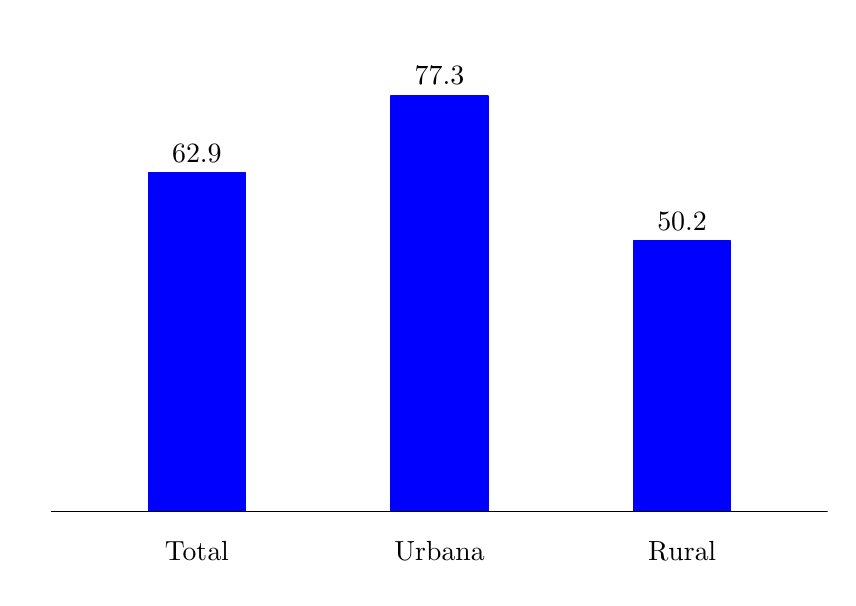
\begin{tikzpicture}[x=1pt,y=1pt]  % Created by tikzDevice version 0.7.0 on 2015-11-25 06:57:15
% !TEX encoding = UTF-8 Unicode
\definecolor[named]{fillColor}{rgb}{1.00,1.00,1.00}
\path[use as bounding box,fill=fillColor,fill opacity=0.00] (0,0) rectangle (289.08,198.74);
\begin{scope}
\path[clip] (  0.00,  0.00) rectangle (289.08,198.74);

\path[] (  0.00,  0.00) rectangle (289.08,198.74);
\end{scope}
\begin{scope}
\path[clip] (  0.00,  0.00) rectangle (289.08,198.74);

\path[] (  8.54, 16.35) rectangle (289.08,181.67);

\path[] ( 61.14, 16.35) --
	( 61.14,181.67);

\path[] (148.81, 16.35) --
	(148.81,181.67);

\path[] (236.48, 16.35) --
	(236.48,181.67);
\definecolor[named]{drawColor}{rgb}{0.00,0.00,1.00}
\definecolor[named]{fillColor}{rgb}{0.00,0.00,1.00}

\path[draw=drawColor,line width= 0.6pt,line join=round,fill=fillColor] ( 43.60, 23.87) rectangle ( 78.67,146.19);

\path[draw=drawColor,line width= 0.6pt,line join=round,fill=fillColor] (131.27, 23.87) rectangle (166.34,174.16);

\path[draw=drawColor,line width= 0.6pt,line join=round,fill=fillColor] (218.94, 23.87) rectangle (254.01,121.55);
\definecolor[named]{drawColor}{rgb}{0.00,0.00,0.00}
\definecolor[named]{fillColor}{rgb}{0.00,0.00,0.00}

\path[draw=drawColor,line width= 0.1pt,line join=round,fill=fillColor] (  8.54, 23.87) -- (289.08, 23.87);

\node[text=drawColor,anchor=base,inner sep=0pt, outer sep=0pt, scale=  1.01] at ( 61.14,150.15) {62.9};

\node[text=drawColor,anchor=base,inner sep=0pt, outer sep=0pt, scale=  1.01] at (148.81,178.11) {77.3};

\node[text=drawColor,anchor=base,inner sep=0pt, outer sep=0pt, scale=  1.01] at (236.48,125.51) {50.2};

\path[] (  8.54, 16.35) rectangle (289.08,181.67);
\end{scope}
\begin{scope}
\path[clip] (  0.00,  0.00) rectangle (289.08,198.74);

\path[] (  8.54, 16.35) --
	(  8.54,181.67);
\end{scope}
\begin{scope}
\path[clip] (  0.00,  0.00) rectangle (289.08,198.74);

\path[] (  8.54, 16.35) --
	(289.08, 16.35);
\end{scope}
\begin{scope}
\path[clip] (  0.00,  0.00) rectangle (289.08,198.74);

\path[] ( 61.14, 12.08) --
	( 61.14, 16.35);

\path[] (148.81, 12.08) --
	(148.81, 16.35);

\path[] (236.48, 12.08) --
	(236.48, 16.35);
\end{scope}
\begin{scope}
\path[clip] (  0.00,  0.00) rectangle (289.08,198.74);
\definecolor[named]{drawColor}{rgb}{0.00,0.00,0.00}

\node[text=drawColor,anchor=base,inner sep=0pt, outer sep=0pt, scale=  1.00] at ( 61.14,  6.04) {Total};

\node[text=drawColor,anchor=base,inner sep=0pt, outer sep=0pt, scale=  1.00] at (148.81,  6.04) {Urbana};

\node[text=drawColor,anchor=base,inner sep=0pt, outer sep=0pt, scale=  1.00] at (236.48,  6.04) {Rural};
\end{scope}
  \end{tikzpicture}}%
{%
 Instituto Nacional de Estadística} %
 
 \cajota{%
Partos con asistencia de personal de salud en los departamentos}%
{%
 El departamento de Guatemala  es donde se observa la mayor atención de partos\footnote{El indicador se calcula con los nacimientos de los cinco años anteriores a la encuesta.} por médico o ginecólogo (94.2\%), mientras que  el de Totonicapán, tiene el menor porcentaje (32.8\%).\\\\ 
Para el departamento de Quiché, uno de cada tres partos son atendidos por médico, mientras que en Huehuetenango y Alta Verapaz, poco más del 38\%.}%
{%
 Proporción de partos con asistencia de médico o ginecólogo} %
{%
 Républica de Guatemala, Encovi 2000, 2006 y 2014, en quetzales de cada año} %
{%
 \includegraphics[width=52\cuadri]{graficas/3_21.pdf}}%
{%
 Instituto Nacional de Estadística} %
 
 \cajita{%
Atención del parto en centros públicos}%
{%
 Nota: para los nacimientos de los cinco años anteriores a cada encuesta.}%
{%
 Proporción de partos con asistencia de médico o ginecólogo} %
{%
 Républica de Guatemala, Encovi 2000, 2006 y 2014, en quetzales de cada año} %
{%
 \begin{tikzpicture}[x=1pt,y=1pt]  % Created by tikzDevice version 0.7.0 on 2015-11-27 14:18:01
% !TEX encoding = UTF-8 Unicode
\definecolor[named]{fillColor}{rgb}{1.00,1.00,1.00}
\path[use as bounding box,fill=fillColor,fill opacity=0.00] (0,0) rectangle (289.08,198.74);
\begin{scope}
\path[clip] (  0.00,  0.00) rectangle (289.08,198.74);

\path[] (  0.00,  0.00) rectangle (289.08,198.74);
\end{scope}
\begin{scope}
\path[clip] (  0.00,  0.00) rectangle (289.08,198.74);

\path[] (  1.64, 17.78) rectangle (280.54,191.48);

\path[] (  1.64, 46.45) --
	(280.54, 46.45);

\path[] (  1.64, 88.01) --
	(280.54, 88.01);

\path[] (  1.64,129.56) --
	(280.54,129.56);

\path[] (  1.64,171.12) --
	(280.54,171.12);

\path[] (  1.64, 25.67) --
	(280.54, 25.67);

\path[] (  1.64, 67.23) --
	(280.54, 67.23);

\path[] (  1.64,108.78) --
	(280.54,108.78);

\path[] (  1.64,150.34) --
	(280.54,150.34);

\path[] ( 41.49, 17.78) --
	( 41.49,191.48);

\path[] (107.89, 17.78) --
	(107.89,191.48);

\path[] (174.30, 17.78) --
	(174.30,191.48);

\path[] (240.70, 17.78) --
	(240.70,191.48);
\definecolor[named]{drawColor}{rgb}{0.00,0.00,1.00}

\path[draw=drawColor,line width= 1.7pt,line join=round] ( 41.49, 62.94) --
	(107.89, 90.49) --
	(174.30,135.28) --
	(240.70,163.62);
\definecolor[named]{drawColor}{rgb}{0.00,0.00,0.00}

\node[text=drawColor,anchor=base,inner sep=0pt, outer sep=0pt, scale=  1.01] at ( 41.49, 51.07) {29.0};

\node[text=drawColor,anchor=base east,inner sep=0pt, outer sep=0pt, scale=  1.01] at (104.78, 90.49) {35.6};

\node[text=drawColor,anchor=base east,inner sep=0pt, outer sep=0pt, scale=  1.01] at (171.18,135.28) {46.4};

\node[text=drawColor,anchor=base,inner sep=0pt, outer sep=0pt, scale=  1.01] at (240.70,167.57) {53.2};
\definecolor[named]{fillColor}{rgb}{0.00,0.00,0.00}

\path[draw=drawColor,line width= 0.1pt,line join=round,fill=fillColor] (  1.64, 25.67) -- (280.54, 25.67);

\path[] (  1.64, 17.78) rectangle (280.54,191.48);
\end{scope}
\begin{scope}
\path[clip] (  0.00,  0.00) rectangle (289.08,198.74);

\path[] (  1.64, 17.78) --
	(  1.64,191.48);
\end{scope}
\begin{scope}
\path[clip] (  0.00,  0.00) rectangle (289.08,198.74);

\path[] (  0.00, 25.67) --
	(  1.64, 25.67);

\path[] (  0.00, 67.23) --
	(  1.64, 67.23);

\path[] (  0.00,108.78) --
	(  1.64,108.78);

\path[] (  0.00,150.34) --
	(  1.64,150.34);
\end{scope}
\begin{scope}
\path[clip] (  0.00,  0.00) rectangle (289.08,198.74);

\path[] (  1.64, 17.78) --
	(280.54, 17.78);
\end{scope}
\begin{scope}
\path[clip] (  0.00,  0.00) rectangle (289.08,198.74);

\path[] ( 41.49, 13.51) --
	( 41.49, 17.78);

\path[] (107.89, 13.51) --
	(107.89, 17.78);

\path[] (174.30, 13.51) --
	(174.30, 17.78);

\path[] (240.70, 13.51) --
	(240.70, 17.78);
\end{scope}
\begin{scope}
\path[clip] (  0.00,  0.00) rectangle (289.08,198.74);
\definecolor[named]{drawColor}{rgb}{0.00,0.00,0.00}

\node[text=drawColor,anchor=base,inner sep=0pt, outer sep=0pt, scale=  1.00] at ( 41.49,  2.85) {2000};

\node[text=drawColor,anchor=base,inner sep=0pt, outer sep=0pt, scale=  1.00] at (107.89,  2.85) {2006};

\node[text=drawColor,anchor=base,inner sep=0pt, outer sep=0pt, scale=  1.00] at (174.30,  2.85) {2011};

\node[text=drawColor,anchor=base,inner sep=0pt, outer sep=0pt, scale=  1.00] at (240.70,  2.85) {2014};
\end{scope}
  \end{tikzpicture}}%
{%
 Instituto Nacional de Estadística} %
 
 \cajita{%
Atención del parto en centros públicos por área de residencia}%
{%
 Para 2014, el 57.3\% de los partos atendidos en el área urbana fue en hospitales, centros y puestos de salud público, mientras que en el área rural, la relacion fue uno de cada dos partos fue atendido en hospitales, centros de salud y puestos de salud públicos. Tanto para el área urbana como para el área rural, la mayor proporción fue en hospitales públicos.}%
{%
 Proporción de partos atendidos en hospital, centro o puesto de salud público por área de residencia} %
{%
 Républica de Guatemala, Encovi 2000, 2006 y 2014, en quetzales de cada año} %
{%
 \begin{tikzpicture}[x=1pt,y=1pt]  \input{graficas/3_23.tex}  \end{tikzpicture}}%
{%
 Instituto Nacional de Estadística} %
 
 \cajota{%
Atención del parto en centros públicos en los departamentos}%
{%
 En los departamentos de Totonicapán y Quiché, menos de la tercera parte de los partos son atendidos en centros de salud público, que incluye puestos, centros y hospitales, y en Sololá y Huehuetenango, poco más del 35\%. Mientras que en los departamentos de Jutiapa, El Progreso y Sacatepéquez, más del 70\% de los partos son atendidos en centros públicos.  }%
{%
 Proporción de partos atendidos en hospital, centro o puesto de salud público por departamento} %
{%
 Républica de Guatemala, Encovi 2000, 2006 y 2014, en quetzales de cada año} %
{%
 \includegraphics[width=52\cuadri]{graficas/3_24.pdf}}%
{%
 Instituto Nacional de Estadística} %
 
 \cajita{%
Acceso a agua mejorada}%
{%
 Nota: incluye tubería dentro de la vivienda, tubería fuera de la vivienda pero en el terreno y chorro público. Para el año 2000, el 72.6\% de la población tenía acceso a mejores fuentes de abastecimiento de agua, que incluye acceso a agua por medio de tubería dentro y fuera de la vivienda y chorro público. De 2000 a 2006, el acceso a agua mejorada aumentó en más de seis puntos porcentuales, no obstante en 2011 se redujo a 75.3\%. Para 2014, se observó que el 77.8\% de los hogares tienen acceso a fuentes mejoradas de abastecimiento de agua.}%
{%
 Proporción de la población con acceso a fuentes mejoradas de abastecimiento de agua potable} %
{%
 Républica de Guatemala, Encovi 2000, 2006 y 2014, en quetzales de cada año} %
{%
 \begin{tikzpicture}[x=1pt,y=1pt]  % Created by tikzDevice version 0.7.0 on 2015-11-26 07:46:48
% !TEX encoding = UTF-8 Unicode
\definecolor[named]{fillColor}{rgb}{1.00,1.00,1.00}
\path[use as bounding box,fill=fillColor,fill opacity=0.00] (0,0) rectangle (289.08,198.74);
\begin{scope}
\path[clip] (  0.00,  0.00) rectangle (289.08,198.74);

\path[] (  0.00,  0.00) rectangle (289.08,198.74);
\end{scope}
\begin{scope}
\path[clip] (  0.00,  0.00) rectangle (289.08,198.74);

\path[] (  1.64, 17.78) rectangle (280.54,191.48);

\path[] (  1.64, 41.46) --
	(280.54, 41.46);

\path[] (  1.64, 73.05) --
	(280.54, 73.05);

\path[] (  1.64,104.63) --
	(280.54,104.63);

\path[] (  1.64,136.21) --
	(280.54,136.21);

\path[] (  1.64,167.80) --
	(280.54,167.80);

\path[] (  1.64, 25.67) --
	(280.54, 25.67);

\path[] (  1.64, 57.25) --
	(280.54, 57.25);

\path[] (  1.64, 88.84) --
	(280.54, 88.84);

\path[] (  1.64,120.42) --
	(280.54,120.42);

\path[] (  1.64,152.00) --
	(280.54,152.00);

\path[] (  1.64,183.59) --
	(280.54,183.59);

\path[] ( 41.49, 17.78) --
	( 41.49,191.48);

\path[] (107.89, 17.78) --
	(107.89,191.48);

\path[] (174.30, 17.78) --
	(174.30,191.48);

\path[] (240.70, 17.78) --
	(240.70,191.48);
\definecolor[named]{drawColor}{rgb}{0.00,0.00,1.00}

\path[draw=drawColor,line width= 1.7pt,line join=round] ( 41.49,128.63) --
	(107.89,147.90) --
	(174.30,137.16) --
	(240.70,145.00);
\definecolor[named]{drawColor}{rgb}{0.00,0.00,0.00}

\node[text=drawColor,anchor=base,inner sep=0pt, outer sep=0pt, scale=  1.01] at ( 41.49,116.76) {72.6};

\node[text=drawColor,anchor=base,inner sep=0pt, outer sep=0pt, scale=  1.01] at (107.89,151.85) {78.7};

\node[text=drawColor,anchor=base,inner sep=0pt, outer sep=0pt, scale=  1.01] at (174.30,125.29) {75.3};

\node[text=drawColor,anchor=base,inner sep=0pt, outer sep=0pt, scale=  1.01] at (240.70,148.96) {77.8};
\definecolor[named]{fillColor}{rgb}{0.00,0.00,0.00}

\path[draw=drawColor,line width= 0.1pt,line join=round,fill=fillColor] (  1.64, 25.67) -- (280.54, 25.67);

\path[] (  1.64, 17.78) rectangle (280.54,191.48);
\end{scope}
\begin{scope}
\path[clip] (  0.00,  0.00) rectangle (289.08,198.74);

\path[] (  1.64, 17.78) --
	(  1.64,191.48);
\end{scope}
\begin{scope}
\path[clip] (  0.00,  0.00) rectangle (289.08,198.74);

\path[] (  0.00, 25.67) --
	(  1.64, 25.67);

\path[] (  0.00, 57.25) --
	(  1.64, 57.25);

\path[] (  0.00, 88.84) --
	(  1.64, 88.84);

\path[] (  0.00,120.42) --
	(  1.64,120.42);

\path[] (  0.00,152.00) --
	(  1.64,152.00);

\path[] (  0.00,183.59) --
	(  1.64,183.59);
\end{scope}
\begin{scope}
\path[clip] (  0.00,  0.00) rectangle (289.08,198.74);

\path[] (  1.64, 17.78) --
	(280.54, 17.78);
\end{scope}
\begin{scope}
\path[clip] (  0.00,  0.00) rectangle (289.08,198.74);

\path[] ( 41.49, 13.51) --
	( 41.49, 17.78);

\path[] (107.89, 13.51) --
	(107.89, 17.78);

\path[] (174.30, 13.51) --
	(174.30, 17.78);

\path[] (240.70, 13.51) --
	(240.70, 17.78);
\end{scope}
\begin{scope}
\path[clip] (  0.00,  0.00) rectangle (289.08,198.74);
\definecolor[named]{drawColor}{rgb}{0.00,0.00,0.00}

\node[text=drawColor,anchor=base,inner sep=0pt, outer sep=0pt, scale=  1.00] at ( 41.49,  2.85) {2000};

\node[text=drawColor,anchor=base,inner sep=0pt, outer sep=0pt, scale=  1.00] at (107.89,  2.85) {2006};

\node[text=drawColor,anchor=base,inner sep=0pt, outer sep=0pt, scale=  1.00] at (174.30,  2.85) {2011};

\node[text=drawColor,anchor=base,inner sep=0pt, outer sep=0pt, scale=  1.00] at (240.70,  2.85) {2014};
\end{scope}
  \end{tikzpicture}}%
{%
 Instituto Nacional de Estadística} %
 
 \cajita{%
Acceso a agua mejorada por área de residencia}%
{%
 Nota: incluye tubería dentro de la vivienda, tubería fuera de la vivienda pero en el terreno y chorro público. Al desagregar por área de residencia se observa que es mayor el acceso a agua mejorada en el área urbana, ya que el 89.1\% tiene acceso a mejores fuentes de abastecimiento de agua, en comparación con el 64.4\% de población que tiene acceso en el área rural.}%
{%
 Proporción de partos con asistencia de médico o ginecólogo} %
{%
 Républica de Guatemala, Encovi 2000, 2006 y 2014, en quetzales de cada año} %
{%
 \begin{tikzpicture}[x=1pt,y=1pt]  \input{graficas/3_26.tex}  \end{tikzpicture}}%
{%
 Instituto Nacional de Estadística} %
 
 \cajota{%
Acceso a agua mejorada en los departamentos}%
{%
  Los departamentos con mayor acceso a mejores fuentes de abastecimiento de agua\footnote{Fuentes mejoradas de abastecimiento de agua potable incluye tubería tanto  dentro de la vivienda como  fuera pero en el terreno, y chorro público.} , son Guatemala, Sacatepéquez y Sololá, con más del 90\% de acceso. 
 
  Por otro lado, en el departamento de Alta Verapaz, menos de la mitad de la población tiene acceso a tubería dentro y fuera de la vivienda o  chorro público.}%
{%
 Proporción de partos con asistencia de médico o ginecólogo} %
{%
 Républica de Guatemala, Encovi 2000, 2006 y 2014, en quetzales de cada año} %
{%
 \includegraphics[width=52\cuadri]{graficas/3_27.pdf}}%
{%
 Instituto Nacional de Estadística} %
 
 \cajita{%
Acceso a saneamiento mejorado}%
{%
 Nota: incluye inodoro conectado a red de drenaje, inodoro conectado a fosa séptica y excusado lavable.}%
{%
 Proporción de partos con asistencia de médico o ginecólogo} %
{%
 Républica de Guatemala, Encovi 2000, 2006 y 2014, en quetzales de cada año} %
{%
 \begin{tikzpicture}[x=1pt,y=1pt]  % Created by tikzDevice version 0.9 on 2015-11-30 18:02:28
% !TEX encoding = UTF-8 Unicode
\definecolor{fillColor}{RGB}{255,255,255}
\path[use as bounding box,fill=fillColor,fill opacity=0.00] (0,0) rectangle (289.08,198.74);
\begin{scope}
\path[clip] (  0.00,  0.00) rectangle (289.08,198.74);

\path[] (  0.00,  0.00) rectangle (289.08,198.74);
\end{scope}
\begin{scope}
\path[clip] (  0.00,  0.00) rectangle (289.08,198.74);

\path[] (  1.64, 17.78) rectangle (280.54,191.48);

\path[] (  1.64, 42.59) --
	(280.54, 42.59);

\path[] (  1.64, 98.99) --
	(280.54, 98.99);

\path[] (  1.64,155.39) --
	(280.54,155.39);

\path[] (  1.64, 70.79) --
	(280.54, 70.79);

\path[] (  1.64,127.19) --
	(280.54,127.19);

\path[] (  1.64,183.59) --
	(280.54,183.59);

\path[] ( 41.49, 17.78) --
	( 41.49,191.48);

\path[] (107.89, 17.78) --
	(107.89,191.48);

\path[] (174.30, 17.78) --
	(174.30,191.48);

\path[] (240.70, 17.78) --
	(240.70,191.48);
\definecolor{drawColor}{RGB}{0,0,255}

\path[draw=drawColor,line width= 1.7pt,line join=round] ( 41.49, 94.48) --
	(107.89,152.57) --
	(174.30,161.03) --
	(240.70,173.86);
\definecolor{drawColor}{RGB}{0,0,0}

\node[text=drawColor,anchor=base,inner sep=0pt, outer sep=0pt, scale=  1.01] at ( 41.49, 82.61) {44.2};

\node[text=drawColor,anchor=base east,inner sep=0pt, outer sep=0pt, scale=  1.01] at (104.78,152.57) {54.5};

\node[text=drawColor,anchor=base east,inner sep=0pt, outer sep=0pt, scale=  1.01] at (171.18,161.03) {56.0};

\node[text=drawColor,anchor=base,inner sep=0pt, outer sep=0pt, scale=  1.01] at (240.70,177.82) {58.3};

\path[draw=drawColor,line width= 0.1pt,line join=round] (  1.64, 25.67) -- (280.54, 25.67);

\path[] (  1.64, 17.78) rectangle (280.54,191.48);
\end{scope}
\begin{scope}
\path[clip] (  0.00,  0.00) rectangle (289.08,198.74);

\path[] (  1.64, 17.78) --
	(  1.64,191.48);
\end{scope}
\begin{scope}
\path[clip] (  0.00,  0.00) rectangle (289.08,198.74);

\path[] (  0.00, 70.79) --
	(  1.64, 70.79);

\path[] (  0.00,127.19) --
	(  1.64,127.19);

\path[] (  0.00,183.59) --
	(  1.64,183.59);
\end{scope}
\begin{scope}
\path[clip] (  0.00,  0.00) rectangle (289.08,198.74);

\path[] (  1.64, 17.78) --
	(280.54, 17.78);
\end{scope}
\begin{scope}
\path[clip] (  0.00,  0.00) rectangle (289.08,198.74);

\path[] ( 41.49, 13.51) --
	( 41.49, 17.78);

\path[] (107.89, 13.51) --
	(107.89, 17.78);

\path[] (174.30, 13.51) --
	(174.30, 17.78);

\path[] (240.70, 13.51) --
	(240.70, 17.78);
\end{scope}
\begin{scope}
\path[clip] (  0.00,  0.00) rectangle (289.08,198.74);
\definecolor{drawColor}{RGB}{0,0,0}

\node[text=drawColor,anchor=base,inner sep=0pt, outer sep=0pt, scale=  1.00] at ( 41.49,  2.85) {2000};

\node[text=drawColor,anchor=base,inner sep=0pt, outer sep=0pt, scale=  1.00] at (107.89,  2.85) {2006};

\node[text=drawColor,anchor=base,inner sep=0pt, outer sep=0pt, scale=  1.00] at (174.30,  2.85) {2011};

\node[text=drawColor,anchor=base,inner sep=0pt, outer sep=0pt, scale=  1.00] at (240.70,  2.85) {2014};
\end{scope}
  \end{tikzpicture}}%
{%
 Instituto Nacional de Estadística} %
 
 \cajita{%
Acceso a saneamiento mejorado por área de residencia}%
{%
 Aunque en promedio casi el 60\% de la población tiene acceso a saneamiento mejorado\footnote{Incluye inodoro conectado a red de drenaje, inodoro conectado a fosa séptica y excusado lavable}, al desagregar por área de residencia se observa que para el área rural, menos del 30\% de los hogares tienen acceso, en comparación con el 83.0\% del área urbana.}%
{%
 Proporción de la población con acceso a servicios de saneamiento mejorados por área de residencia} %
{%
 Républica de Guatemala, Encovi 2000, 2006 y 2014, en quetzales de cada año} %
{%
 \begin{tikzpicture}[x=1pt,y=1pt]  \input{graficas/3_29.tex}  \end{tikzpicture}}%
{%
 Instituto Nacional de Estadística} %
 
 \cajota{%
Acceso a saneamiento mejorado en los departamentos}%
{%
 El 21.4\% de los hogares en Alta Verapaz y el 30.1\% en Totonicapán tiene acceso a saneamiento mejorado, mientras que en los departamentos de Guatemala y Sacatepéquez, casi el 90\% de los hogares cuenta con servicios de saneamiento mejorados.}%
{%
 Proporción de la población con acceso a servicios de saneamiento mejorados } %
{%
 Républica de Guatemala, Encovi 2000, 2006 y 2014, en quetzales de cada año} %
{%
 \includegraphics[width=52\cuadri]{graficas/3_30.pdf}}%
{%
 Instituto Nacional de Estadística} %
  
%
 \cajita{%
Población con gastos inferiores a la línea de pobreza extrema}%
{%
 Este indicador muestra el porcentaje de población cuyo consumo es inferior a la línea de pobreza extrema\footnote{Para 2014, este valor era de Q 5,750 por persona al año.}, es decir, corresponde al grupo de población que no logra cubrir el costo del consumo mínimo de alimentos. 
 
En la gráfica se advierte que entre 2000 y 2006,  la pobreza extrema se mantuvo casi  al mismo nivel; no obstante en  2014 se observó un aumento de 8.2 puntos porcentuales.}%
{%
 Proporción de partos con asistencia de médico o ginecólogo} %
{%
 Républica de Guatemala, Encovi 2000, 2006 y 2014, en quetzales de cada año} %
{%
 \begin{tikzpicture}[x=1pt,y=1pt]  % Created by tikzDevice version 0.7.0 on 2015-11-27 14:11:58
% !TEX encoding = UTF-8 Unicode
\definecolor[named]{fillColor}{rgb}{1.00,1.00,1.00}
\path[use as bounding box,fill=fillColor,fill opacity=0.00] (0,0) rectangle (289.08,198.74);
\begin{scope}
\path[clip] (  0.00,  0.00) rectangle (289.08,198.74);

\path[] (  0.00,  0.00) rectangle (289.08,198.74);
\end{scope}
\begin{scope}
\path[clip] (  0.00,  0.00) rectangle (289.08,198.74);

\path[] (  1.64, 17.78) rectangle (280.54,191.48);

\path[] (  1.64, 53.87) --
	(280.54, 53.87);

\path[] (  1.64,110.27) --
	(280.54,110.27);

\path[] (  1.64,166.67) --
	(280.54,166.67);

\path[] (  1.64, 25.67) --
	(280.54, 25.67);

\path[] (  1.64, 82.07) --
	(280.54, 82.07);

\path[] (  1.64,138.47) --
	(280.54,138.47);

\path[] ( 53.94, 17.78) --
	( 53.94,191.48);

\path[] (141.09, 17.78) --
	(141.09,191.48);

\path[] (228.25, 17.78) --
	(228.25,191.48);
\definecolor[named]{drawColor}{rgb}{0.00,0.00,1.00}

\path[draw=drawColor,line width= 1.7pt,line join=round] ( 53.94,114.42) --
	(141.09,111.40) --
	(228.25,157.40);
\definecolor[named]{drawColor}{rgb}{0.00,0.00,0.00}

\node[text=drawColor,anchor=base,inner sep=0pt, outer sep=0pt, scale=  1.01] at ( 53.94,118.38) {15.7};

\node[text=drawColor,anchor=base,inner sep=0pt, outer sep=0pt, scale=  1.01] at (141.09, 99.53) {15.2};

\node[text=drawColor,anchor=base,inner sep=0pt, outer sep=0pt, scale=  1.01] at (228.25,161.35) {23.4};
\definecolor[named]{fillColor}{rgb}{0.00,0.00,0.00}

\path[draw=drawColor,line width= 0.1pt,line join=round,fill=fillColor] (  1.64, 25.67) -- (280.54, 25.67);

\path[] (  1.64, 17.78) rectangle (280.54,191.48);
\end{scope}
\begin{scope}
\path[clip] (  0.00,  0.00) rectangle (289.08,198.74);

\path[] (  1.64, 17.78) --
	(  1.64,191.48);
\end{scope}
\begin{scope}
\path[clip] (  0.00,  0.00) rectangle (289.08,198.74);

\path[] (  0.00, 25.67) --
	(  1.64, 25.67);

\path[] (  0.00, 82.07) --
	(  1.64, 82.07);

\path[] (  0.00,138.47) --
	(  1.64,138.47);
\end{scope}
\begin{scope}
\path[clip] (  0.00,  0.00) rectangle (289.08,198.74);

\path[] (  1.64, 17.78) --
	(280.54, 17.78);
\end{scope}
\begin{scope}
\path[clip] (  0.00,  0.00) rectangle (289.08,198.74);

\path[] ( 53.94, 13.51) --
	( 53.94, 17.78);

\path[] (141.09, 13.51) --
	(141.09, 17.78);

\path[] (228.25, 13.51) --
	(228.25, 17.78);
\end{scope}
\begin{scope}
\path[clip] (  0.00,  0.00) rectangle (289.08,198.74);
\definecolor[named]{drawColor}{rgb}{0.00,0.00,0.00}

\node[text=drawColor,anchor=base,inner sep=0pt, outer sep=0pt, scale=  1.00] at ( 53.94,  2.85) {2000};

\node[text=drawColor,anchor=base,inner sep=0pt, outer sep=0pt, scale=  1.00] at (141.09,  2.85) {2006};

\node[text=drawColor,anchor=base,inner sep=0pt, outer sep=0pt, scale=  1.00] at (228.25,  2.85) {2014};
\end{scope}
  \end{tikzpicture}}%
{%
 Instituto Nacional de Estadística} %
 
 \cajita{%
Población con gastos inferiores a la línea de pobreza extrema por área de residencia}%
{%
 Para 2014, la mitad de la población guatemalteca habitaba en áreas rurales. Al desagregar por área de residencia a la población que se encuentra por debajo de la línea de pobreza extrema, se obtiene que más de la tercera parte de la población que habita en áreas rurales es extremadamente pobre, en comparación con 11.2\% en el área urbana.}%
{%
 Proporción de partos con asistencia de médico o ginecólogo} %
{%
 Républica de Guatemala, Encovi 2000, 2006 y 2014, en quetzales de cada año} %
{%
 \begin{tikzpicture}[x=1pt,y=1pt]  \input{graficas/3_02.tex}  \end{tikzpicture}}%
{%
 Instituto Nacional de Estadística} %
 
 \cajota{%
Población con gastos inferiores a la línea de pobreza extrema en los departamentos}%
{%
 Los departamentos de Alta Verapaz, Quiché, Chiquimula y Totonicapán, muestran los porcentajes de pobreza extrema más elevados, por encima del promedio nacional. Incluso para el departamento de Alta Verapaz, la pobreza extrema es más del doble del promedio nacional. Mientras que en los departamentos de Sacatepéquez y Guatemala, la pobreza extrema es menos del 10\%.}%
{%
 Proporción de la población que se encuentra por debajo de la línea de pobreza extrema por departamento} %
{%
 Républica de Guatemala, Encovi 2000, 2006 y 2014, en quetzales de cada año} %
{%
 \includegraphics[width=52\cuadri]{graficas/3_03.pdf}}%
{%
 Instituto Nacional de Estadística} %
 
 \cajita{%
Consumo Nacional de la quinta parte de la población más pobre}%
{%
 La participación de cada quintil en el consumo nacional, es un indicador que permite evidenciar las  desigualdades entre los distintos estratos de la población. \\\\ 
Para el 2014, el 20\% más  pobre de la población captaba el 7.1\% del consumo nacional. Se puede observar que entre 2000 y 2014, la participación del quintil más pobre aumentó de 5.2\% en 2000 a 7.1\%  en 2014.}%
{%
 Proporción del consumo nacional que corresponde al quintil más pobre de la población} %
{%
 Serie histórica por Encovi, en porcentaje} %
{%
 \begin{tikzpicture}[x=1pt,y=1pt]  % Created by tikzDevice version 0.9 on 2015-11-30 18:02:16
% !TEX encoding = UTF-8 Unicode
\definecolor{fillColor}{RGB}{255,255,255}
\path[use as bounding box,fill=fillColor,fill opacity=0.00] (0,0) rectangle (289.08,198.74);
\begin{scope}
\path[clip] (  0.00,  0.00) rectangle (289.08,198.74);

\path[] (  0.00,  0.00) rectangle (289.08,198.74);
\end{scope}
\begin{scope}
\path[clip] (  0.00,  0.00) rectangle (289.08,198.74);

\path[] ( -2.73, 17.78) rectangle (280.54,191.48);

\path[] (  0.00, 25.67) --
	(280.54, 25.67);

\path[] (  0.00, 70.79) --
	(280.54, 70.79);

\path[] (  0.00,115.91) --
	(280.54,115.91);

\path[] (  0.00,161.03) --
	(280.54,161.03);

\path[] (  0.00, 48.23) --
	(280.54, 48.23);

\path[] (  0.00, 93.35) --
	(280.54, 93.35);

\path[] (  0.00,138.47) --
	(280.54,138.47);

\path[] (  0.00,183.59) --
	(280.54,183.59);

\path[] ( 50.38, 17.78) --
	( 50.38,191.48);

\path[] (138.90, 17.78) --
	(138.90,191.48);

\path[] (227.43, 17.78) --
	(227.43,191.48);
\definecolor{drawColor}{RGB}{0,0,255}

\path[draw=drawColor,line width= 1.7pt,line join=round] ( 50.38,119.75) --
	(138.90,129.77) --
	(227.43,162.39);
\definecolor{drawColor}{RGB}{0,0,0}

\node[text=drawColor,anchor=base,inner sep=0pt, outer sep=0pt, scale=  1.01] at ( 50.38,107.88) {5.2};

\node[text=drawColor,anchor=base east,inner sep=0pt, outer sep=0pt, scale=  1.01] at (136.67,129.77) {5.6};

\node[text=drawColor,anchor=base,inner sep=0pt, outer sep=0pt, scale=  1.01] at (227.43,166.34) {7.1};

\path[draw=drawColor,line width= 0.1pt,line join=round] (  0.00, 25.67) -- (280.54, 25.67);

\path[] ( -2.73, 17.78) rectangle (280.54,191.48);
\end{scope}
\begin{scope}
\path[clip] (  0.00,  0.00) rectangle (289.08,198.74);

\path[] (  0.00, 17.78) --
	(280.54, 17.78);
\end{scope}
\begin{scope}
\path[clip] (  0.00,  0.00) rectangle (289.08,198.74);

\path[] ( 50.38, 13.51) --
	( 50.38, 17.78);

\path[] (138.90, 13.51) --
	(138.90, 17.78);

\path[] (227.43, 13.51) --
	(227.43, 17.78);
\end{scope}
\begin{scope}
\path[clip] (  0.00,  0.00) rectangle (289.08,198.74);
\definecolor{drawColor}{RGB}{0,0,0}

\node[text=drawColor,anchor=base,inner sep=0pt, outer sep=0pt, scale=  1.00] at ( 50.38,  2.85) {2000};

\node[text=drawColor,anchor=base,inner sep=0pt, outer sep=0pt, scale=  1.00] at (138.90,  2.85) {2006};

\node[text=drawColor,anchor=base,inner sep=0pt, outer sep=0pt, scale=  1.00] at (227.43,  2.85) {2014};
\end{scope}
  \end{tikzpicture}}%
{%
 Instituto Nacional de Estadística} %
 
 \cajita{%
Consumo Nacional del quintil más pobre por área de residencia}%
{%
 En el área urbana el 20\% más pobre de la población    capta  el 2.5\% del consumo total, dato menor al del promedio nacional.

Mientras que en el área rural el quintil\footnote{Un quintil es la quinta parte de una población estadística ordenada de menor a mayor en alguna característica de esta.} más pobre,  capta el 15.1\% del consumo.}%
{%
 Proporción del consumo nacional que corresponde al quintil más pobre de la población por área de residencia} %
{%
 Républica de Guatemala, Encovi 2000, 2006 y 2014, en quetzales de cada año} %
{%
 \begin{tikzpicture}[x=1pt,y=1pt]  \input{graficas/3_05.tex}  \end{tikzpicture}}%
{%
 Instituto Nacional de Estadística} %
 
 \cajita{%
Empleo pleno y productivo}%
{%
 Nota: población ocupada de 15 años o más como proporción de la población de 15 años o mas. Este indicador muestra la capacidad de la economía de generar empleo. Es un indicador cuantitativo y no refleja la calidad del empleo a lo largo del tiempo, ya que se considera al total de la población ocupada.  Entre 2000 y 2014, la relación entre empleo y población se ha mantenido por encima del 60\%, variando de 62.7\% en el 2000 a 60.8\% en el 2014.}%
{%
 Proporción de partos con asistencia de médico o ginecólogo} %
{%
 Républica de Guatemala, Encovi 2000, 2006 y 2014, en quetzales de cada año} %
{%
 \begin{tikzpicture}[x=1pt,y=1pt]  % Created by tikzDevice version 0.7.0 on 2015-11-25 08:00:33
% !TEX encoding = UTF-8 Unicode
\definecolor[named]{fillColor}{rgb}{1.00,1.00,1.00}
\path[use as bounding box,fill=fillColor,fill opacity=0.00] (0,0) rectangle (289.08,198.74);
\begin{scope}
\path[clip] (  0.00,  0.00) rectangle (289.08,198.74);

\path[] (  0.00,  0.00) rectangle (289.08,198.74);
\end{scope}
\begin{scope}
\path[clip] (  0.00,  0.00) rectangle (289.08,198.74);

\path[] (  1.64, 17.78) rectangle (280.54,191.48);

\path[] (  1.64, 43.62) --
	(280.54, 43.62);

\path[] (  1.64, 79.51) --
	(280.54, 79.51);

\path[] (  1.64,115.40) --
	(280.54,115.40);

\path[] (  1.64,151.29) --
	(280.54,151.29);

\path[] (  1.64,187.18) --
	(280.54,187.18);

\path[] (  1.64, 25.67) --
	(280.54, 25.67);

\path[] (  1.64, 61.56) --
	(280.54, 61.56);

\path[] (  1.64, 97.45) --
	(280.54, 97.45);

\path[] (  1.64,133.34) --
	(280.54,133.34);

\path[] (  1.64,169.23) --
	(280.54,169.23);

\path[] ( 41.49, 17.78) --
	( 41.49,191.48);

\path[] (107.89, 17.78) --
	(107.89,191.48);

\path[] (174.30, 17.78) --
	(174.30,191.48);

\path[] (240.70, 17.78) --
	(240.70,191.48);
\definecolor[named]{drawColor}{rgb}{0.00,0.00,1.00}

\path[draw=drawColor,line width= 1.7pt,line join=round] ( 41.49,152.91) --
	(107.89,168.46) --
	(174.30,153.54) --
	(240.70,139.25);
\definecolor[named]{drawColor}{rgb}{0.00,0.00,0.00}

\node[text=drawColor,anchor=base,inner sep=0pt, outer sep=0pt, scale=  1.01] at ( 41.49,141.04) {62.7};

\node[text=drawColor,anchor=base,inner sep=0pt, outer sep=0pt, scale=  1.01] at (107.89,172.42) {64.9};

\node[text=drawColor,anchor=base west,inner sep=0pt, outer sep=0pt, scale=  1.01] at (174.30,157.49) {62.8};

\node[text=drawColor,anchor=base,inner sep=0pt, outer sep=0pt, scale=  1.01] at (240.70,127.38) {60.8};
\definecolor[named]{fillColor}{rgb}{0.00,0.00,0.00}

\path[draw=drawColor,line width= 0.1pt,line join=round,fill=fillColor] (  1.64, 25.67) -- (280.54, 25.67);

\path[] (  1.64, 17.78) rectangle (280.54,191.48);
\end{scope}
\begin{scope}
\path[clip] (  0.00,  0.00) rectangle (289.08,198.74);

\path[] (  1.64, 17.78) --
	(  1.64,191.48);
\end{scope}
\begin{scope}
\path[clip] (  0.00,  0.00) rectangle (289.08,198.74);

\path[] (  0.00, 25.67) --
	(  1.64, 25.67);

\path[] (  0.00, 61.56) --
	(  1.64, 61.56);

\path[] (  0.00, 97.45) --
	(  1.64, 97.45);

\path[] (  0.00,133.34) --
	(  1.64,133.34);

\path[] (  0.00,169.23) --
	(  1.64,169.23);
\end{scope}
\begin{scope}
\path[clip] (  0.00,  0.00) rectangle (289.08,198.74);

\path[] (  1.64, 17.78) --
	(280.54, 17.78);
\end{scope}
\begin{scope}
\path[clip] (  0.00,  0.00) rectangle (289.08,198.74);

\path[] ( 41.49, 13.51) --
	( 41.49, 17.78);

\path[] (107.89, 13.51) --
	(107.89, 17.78);

\path[] (174.30, 13.51) --
	(174.30, 17.78);

\path[] (240.70, 13.51) --
	(240.70, 17.78);
\end{scope}
\begin{scope}
\path[clip] (  0.00,  0.00) rectangle (289.08,198.74);
\definecolor[named]{drawColor}{rgb}{0.00,0.00,0.00}

\node[text=drawColor,anchor=base,inner sep=0pt, outer sep=0pt, scale=  1.00] at ( 41.49,  2.85) {2000};

\node[text=drawColor,anchor=base,inner sep=0pt, outer sep=0pt, scale=  1.00] at (107.89,  2.85) {2006};

\node[text=drawColor,anchor=base,inner sep=0pt, outer sep=0pt, scale=  1.00] at (174.30,  2.85) {2011};

\node[text=drawColor,anchor=base,inner sep=0pt, outer sep=0pt, scale=  1.00] at (240.70,  2.85) {2014};
\end{scope}
  \end{tikzpicture}}%
{%
 Instituto Nacional de Estadística} %
 
 \cajita{%
Empleo pleno y productivo por área de residencia}%
{%
 \textollamada{El indicador relación empleo-población se obtiene al dividir la población ocupada de 15 años o más,  entre la población mayor de 14 años.} Al desagregar por área de residencia se obtiene que la relación entre empleo y población es mayor en el área urbana que en el área rural, 62.8\% y 58.6\%, respectivamente. Es decir, que la capacidad de la economía para generar empleo es un poco mayor en el área urbana que en el área rural.}%
{%
 Relación entre empleo y población por área de residencia} %
{%
 Républica de Guatemala, Encovi 2000, 2006 y 2014, en quetzales de cada año} %
{%
 \begin{tikzpicture}[x=1pt,y=1pt]  \input{graficas/3_08.tex}  \end{tikzpicture}}%
{%
 Instituto Nacional de Estadística} %
 
 \cajota{%
Empleo pleno y productivo en los departamentos}%
{%
 \textollamada[*][*]{El indicador relación empleo-población se obtiene al dividir la población ocupada de 15 años o más,  entre la población mayor de 14 años multiplicada por 100.}Conocer las diferencias en la relación empleo-población en los departamentos es útil para la focalización de políticas públicas en materia de generación de empleo. 

 Los departamentos de Zacapa, Chimaltenango y Alta Verapaz, muestran una mayor capacidad para generar empleo, con una relación empleo-población por encima del 65\%, mientras que en los departamentos Jutiapa y El Progreso, la relación es menor al 55\%.
}%
{%
 Relación entre empleo y población} %
{%
 Por departamento, Encovi 2014, en porcentaje} %
{%
 \includegraphics[width=52\cuadri]{graficas/3_09.pdf}}%
{%
 Instituto Nacional de Estadística} %
 
 \cajita{%
Población ocupada no asalariada}%
{%
 La población ocupada\footnote{Personas de 15 años o más, que durante la semana de referencia hayan realizado durante una hora o un día, alguna actividad económica, trabajando en el período de referencia por un sueldo o salario en metálico o especie o ausentes temporalmente de su trabajo} no asalariada que trabaja por cuenta propia, no posee una relación contractual, ni goza de los beneficios de aguinaldo, bono 14, horas extras, etc., además de no tener acceso a seguridad social.

 Para 2000, casi   la tercera parte de los ocupados trabajaba de forma independiente. Esta proporción se redujo en el 2014 a 26.4\%.}%
{%
 Proporción de partos con asistencia de médico o ginecólogo} %
{%
 Républica de Guatemala, Encovi 2000, 2006 y 2014, en quetzales de cada año} %
{%
 \begin{tikzpicture}[x=1pt,y=1pt]  % Created by tikzDevice version 0.9 on 2015-11-24 22:44:22
% !TEX encoding = UTF-8 Unicode
\definecolor{fillColor}{RGB}{255,255,255}
\path[use as bounding box,fill=fillColor,fill opacity=0.00] (0,0) rectangle (289.08,198.74);
\begin{scope}
\path[clip] (  0.00,  0.00) rectangle (289.08,198.74);

\path[] (  0.00,  0.00) rectangle (289.08,198.74);
\end{scope}
\begin{scope}
\path[clip] (  0.00,  0.00) rectangle (289.08,198.74);

\path[] (  1.64, 17.78) rectangle (280.54,191.48);

\path[] (  1.64, 27.09) --
	(280.54, 27.09);

\path[] (  1.64, 77.37) --
	(280.54, 77.37);

\path[] (  1.64,127.64) --
	(280.54,127.64);

\path[] (  1.64,177.92) --
	(280.54,177.92);

\path[] (  1.64, 52.23) --
	(280.54, 52.23);

\path[] (  1.64,102.51) --
	(280.54,102.51);

\path[] (  1.64,152.78) --
	(280.54,152.78);

\path[] ( 41.49, 17.78) --
	( 41.49,191.48);

\path[] (107.89, 17.78) --
	(107.89,191.48);

\path[] (174.30, 17.78) --
	(174.30,191.48);

\path[] (240.70, 17.78) --
	(240.70,191.48);
\definecolor{drawColor}{RGB}{0,0,255}

\path[draw=drawColor,line width= 1.7pt,line join=round] ( 41.49,183.59) --
	(107.89,179.02) --
	(174.30, 89.24) --
	(240.70, 62.11);
\definecolor{drawColor}{RGB}{0,0,0}

\node[text=drawColor,anchor=base,inner sep=0pt, outer sep=0pt, scale=  1.01] at ( 41.49,187.54) {31.23};

\node[text=drawColor,anchor=base west,inner sep=0pt, outer sep=0pt, scale=  1.01] at (107.89,182.97) {31.04};

\node[text=drawColor,anchor=base west,inner sep=0pt, outer sep=0pt, scale=  1.01] at (174.30, 93.20) {27.47};

\node[text=drawColor,anchor=base,inner sep=0pt, outer sep=0pt, scale=  1.01] at (240.70, 50.24) {26.39};

\path[draw=drawColor,line width= 0.1pt,line join=round] (  1.64, 25.67) -- (280.54, 25.67);

\path[] (  1.64, 17.78) rectangle (280.54,191.48);
\end{scope}
\begin{scope}
\path[clip] (  0.00,  0.00) rectangle (289.08,198.74);

\path[] (  1.64, 17.78) --
	(  1.64,191.48);
\end{scope}
\begin{scope}
\path[clip] (  0.00,  0.00) rectangle (289.08,198.74);

\path[] (  0.00, 52.23) --
	(  1.64, 52.23);

\path[] (  0.00,102.51) --
	(  1.64,102.51);

\path[] (  0.00,152.78) --
	(  1.64,152.78);
\end{scope}
\begin{scope}
\path[clip] (  0.00,  0.00) rectangle (289.08,198.74);

\path[] (  1.64, 17.78) --
	(280.54, 17.78);
\end{scope}
\begin{scope}
\path[clip] (  0.00,  0.00) rectangle (289.08,198.74);

\path[] ( 41.49, 13.51) --
	( 41.49, 17.78);

\path[] (107.89, 13.51) --
	(107.89, 17.78);

\path[] (174.30, 13.51) --
	(174.30, 17.78);

\path[] (240.70, 13.51) --
	(240.70, 17.78);
\end{scope}
\begin{scope}
\path[clip] (  0.00,  0.00) rectangle (289.08,198.74);
\definecolor{drawColor}{RGB}{0,0,0}

\node[text=drawColor,anchor=base,inner sep=0pt, outer sep=0pt, scale=  1.00] at ( 41.49,  2.85) {2000};

\node[text=drawColor,anchor=base,inner sep=0pt, outer sep=0pt, scale=  1.00] at (107.89,  2.85) {2006};

\node[text=drawColor,anchor=base,inner sep=0pt, outer sep=0pt, scale=  1.00] at (174.30,  2.85) {2011};

\node[text=drawColor,anchor=base,inner sep=0pt, outer sep=0pt, scale=  1.00] at (240.70,  2.85) {2014};
\end{scope}
  \end{tikzpicture}}%
{%
 Instituto Nacional de Estadística} %
 
 \cajita{%
Población ocupada no asalariada por área de residencia}%
{%
 La proporción de la población que trabaja por cuenta propia, agrícola y no agrícola, es mayor en el área rural que en el área urbana, la diferencia es poco más de cinco puntos porcentuales. Es decir, que en el área rural es mayor la proporción de ocupados sin acceso a una relación contractual y a otros beneficios.}%
{%
 Proporción de la población ocupada que trabaja por cuenta propia o en una empresa familiar por área de residencia} %
{%
 Républica de Guatemala, Encovi 2000, 2006 y 2014, en quetzales de cada año} %
{%
 \begin{tikzpicture}[x=1pt,y=1pt]  \input{graficas/3_11.tex}  \end{tikzpicture}}%
{%
 Instituto Nacional de Estadística} %
 
 \cajota{%
Población ocupada no asalariada en los departamentos}%
{%
 En Jutiapa, Huehuetenango y  Quiché más de la tercera parte de la población ocupada trabaja por cuenta propia o en una empresa familiar, por encima del promedio nacional (26.4\%). 

Por otro lado,  los departamentos de Escuintla, Izabal,  y Quetzaltenango son los que tienen el porcentaje de población ocupada no asalariada más bajos. }%
{%
 Proporción de la población ocupada que trabaja por cuenta propia o en una empresa familiar por departamento} %
{%
 Républica de Guatemala, Encovi 2000, 2006 y 2014, en quetzales de cada año} %
{%
 \includegraphics[width=52\cuadri]{graficas/3_12.pdf}}%
{%
 Instituto Nacional de Estadística} %
 
 \cajita{%
Alfabetismo en jóvenes}%
{%
 La tasa de alfabetismo\footnote{Cualidad o estado de las personas que saben leer y escribir.} de las personas entre 15 y 24 años, aumentó entre 2000 y 2014, en más de 10 puntos porcentuales. 

Para el año 2000, 2 de cada 10 \mbox{personas} de 15 a 24 años no podía leer y escribir, mientras que para 2014, esta proporción se redujo a cerca de 1 de cada 10 personas.}%
{%
 Proporción de partos con asistencia de médico o ginecólogo} %
{%
 Républica de Guatemala, Encovi 2000, 2006 y 2014, en quetzales de cada año} %
{%
 \begin{tikzpicture}[x=1pt,y=1pt]  % Created by tikzDevice version 0.7.0 on 2015-11-25 08:27:02
% !TEX encoding = UTF-8 Unicode
\definecolor[named]{fillColor}{rgb}{1.00,1.00,1.00}
\path[use as bounding box,fill=fillColor,fill opacity=0.00] (0,0) rectangle (289.08,198.74);
\begin{scope}
\path[clip] (  0.00,  0.00) rectangle (289.08,198.74);

\path[] (  0.00,  0.00) rectangle (289.08,198.74);
\end{scope}
\begin{scope}
\path[clip] (  0.00,  0.00) rectangle (289.08,198.74);

\path[] (  6.02, 17.78) rectangle (280.54,191.48);

\path[] (  6.02, 25.67) --
	(280.54, 25.67);

\path[] (  6.02, 61.56) --
	(280.54, 61.56);

\path[] (  6.02, 97.45) --
	(280.54, 97.45);

\path[] (  6.02,133.34) --
	(280.54,133.34);

\path[] (  6.02,169.23) --
	(280.54,169.23);

\path[] (  6.02, 43.62) --
	(280.54, 43.62);

\path[] (  6.02, 79.51) --
	(280.54, 79.51);

\path[] (  6.02,115.40) --
	(280.54,115.40);

\path[] (  6.02,151.29) --
	(280.54,151.29);

\path[] (  6.02,187.18) --
	(280.54,187.18);

\path[] ( 45.24, 17.78) --
	( 45.24,191.48);

\path[] (110.60, 17.78) --
	(110.60,191.48);

\path[] (175.96, 17.78) --
	(175.96,191.48);

\path[] (241.33, 17.78) --
	(241.33,191.48);
\definecolor[named]{drawColor}{rgb}{0.00,0.00,1.00}

\path[draw=drawColor,line width= 1.7pt,line join=round] ( 45.24,121.50) --
	(110.60,143.39) --
	(175.96,155.23) --
	(241.33,163.29);
\definecolor[named]{drawColor}{rgb}{0.00,0.00,0.00}

\node[text=drawColor,anchor=base,inner sep=0pt, outer sep=0pt, scale=  1.01] at ( 45.24,109.63) {81.7};

\node[text=drawColor,anchor=base east,inner sep=0pt, outer sep=0pt, scale=  1.01] at (107.49,143.39) {87.8};

\node[text=drawColor,anchor=base east,inner sep=0pt, outer sep=0pt, scale=  1.01] at (172.85,155.23) {91.1};

\node[text=drawColor,anchor=base,inner sep=0pt, outer sep=0pt, scale=  1.01] at (241.33,167.25) {93.3};
\definecolor[named]{fillColor}{rgb}{0.00,0.00,0.00}

\path[draw=drawColor,line width= 0.1pt,line join=round,fill=fillColor] (  6.02, 25.67) -- (280.54, 25.67);

\path[] (  6.02, 17.78) rectangle (280.54,191.48);
\end{scope}
\begin{scope}
\path[clip] (  0.00,  0.00) rectangle (289.08,198.74);

\path[] (  6.02, 17.78) --
	(  6.02,191.48);
\end{scope}
\begin{scope}
\path[clip] (  0.00,  0.00) rectangle (289.08,198.74);

\path[] (  1.76, 43.62) --
	(  6.02, 43.62);

\path[] (  1.76, 79.51) --
	(  6.02, 79.51);

\path[] (  1.76,115.40) --
	(  6.02,115.40);

\path[] (  1.76,151.29) --
	(  6.02,151.29);

\path[] (  1.76,187.18) --
	(  6.02,187.18);
\end{scope}
\begin{scope}
\path[clip] (  0.00,  0.00) rectangle (289.08,198.74);

\path[] (  6.02, 17.78) --
	(280.54, 17.78);
\end{scope}
\begin{scope}
\path[clip] (  0.00,  0.00) rectangle (289.08,198.74);

\path[] ( 45.24, 13.51) --
	( 45.24, 17.78);

\path[] (110.60, 13.51) --
	(110.60, 17.78);

\path[] (175.96, 13.51) --
	(175.96, 17.78);

\path[] (241.33, 13.51) --
	(241.33, 17.78);
\end{scope}
\begin{scope}
\path[clip] (  0.00,  0.00) rectangle (289.08,198.74);
\definecolor[named]{drawColor}{rgb}{0.00,0.00,0.00}

\node[text=drawColor,anchor=base,inner sep=0pt, outer sep=0pt, scale=  1.00] at ( 45.24,  2.85) {2000};

\node[text=drawColor,anchor=base,inner sep=0pt, outer sep=0pt, scale=  1.00] at (110.60,  2.85) {2006};

\node[text=drawColor,anchor=base,inner sep=0pt, outer sep=0pt, scale=  1.00] at (175.96,  2.85) {2011};

\node[text=drawColor,anchor=base,inner sep=0pt, outer sep=0pt, scale=  1.00] at (241.33,  2.85) {2014};
\end{scope}
  \end{tikzpicture}}%
{%
 Instituto Nacional de Estadística} %
 
 \cajita{%
Alfabetismo en jóvenes por área de residencia}%
{%
  Al desagregar la proporción de partos con asistencia de personal de salud especializado\footnote{El indicador se calcula con los nacimientos de los cinco años anteriores a la encuesta.} por área de residencia, se obtiene que tres de cada cuatro partos en el área urbana son atendidos por médico o ginecólogo, mientras que para el área rural, la relación es de  dos de cada cuatro partos.}%
{%
 Tasa de alfabetismo en jóvenes de 15 a 24 años por área de residencia} %
{%
 República de Guatemala, Encovi 2014, en porcentaje} %
{%
 \begin{tikzpicture}[x=1pt,y=1pt]  \input{graficas/3_14.tex}  \end{tikzpicture}}%
{%
 Instituto Nacional de Estadística} %
 
 \cajota{%
Alfabetismo en jóvenes en los departamentos}%
{%
  Al desagregar la proporción de partos con asistencia de personal de salud especializado\footnote{El indicador se calcula con los nacimientos de los cinco años anteriores a la encuesta.} por área de residencia, se obtiene que tres de cada cuatro partos en el área urbana son atendidos por médico o ginecólogo, mientras que para el área rural, la relación es de  dos de cada cuatro partos.}%
{%
 Tasa de alfabetismo en personas de 15 a 24 años } %
{%
 Encovi 2014, en porcentaje} %
{%
 \includegraphics[width=52\cuadri]{graficas/3_15.pdf}}%
{%
 Instituto Nacional de Estadística} %
 
 \cajita{%
Mujeres empleadas remuneradas en el sector no agrícola}%
{%
 Nota: mujeres ocupadas remuneradas en el sector no agrícola como proporción de la población ocupada remunerada en el sector no agrícola.}%
{%
 Proporción de partos con asistencia de médico o ginecólogo} %
{%
 Républica de Guatemala, Encovi 2000, 2006 y 2014, en quetzales de cada año} %
{%
 \begin{tikzpicture}[x=1pt,y=1pt]  % Created by tikzDevice version 0.9 on 2015-11-30 18:02:23
% !TEX encoding = UTF-8 Unicode
\definecolor{fillColor}{RGB}{255,255,255}
\path[use as bounding box,fill=fillColor,fill opacity=0.00] (0,0) rectangle (289.08,198.74);
\begin{scope}
\path[clip] (  0.00,  0.00) rectangle (289.08,198.74);

\path[] (  0.00,  0.00) rectangle (289.08,198.74);
\end{scope}
\begin{scope}
\path[clip] (  0.00,  0.00) rectangle (289.08,198.74);

\path[] (  1.64, 17.78) rectangle (280.54,191.48);

\path[] (  1.64, 50.35) --
	(280.54, 50.35);

\path[] (  1.64, 99.69) --
	(280.54, 99.69);

\path[] (  1.64,149.04) --
	(280.54,149.04);

\path[] (  1.64, 25.67) --
	(280.54, 25.67);

\path[] (  1.64, 75.02) --
	(280.54, 75.02);

\path[] (  1.64,124.37) --
	(280.54,124.37);

\path[] (  1.64,173.72) --
	(280.54,173.72);

\path[] ( 41.49, 17.78) --
	( 41.49,191.48);

\path[] (107.89, 17.78) --
	(107.89,191.48);

\path[] (174.30, 17.78) --
	(174.30,191.48);

\path[] (240.70, 17.78) --
	(240.70,191.48);
\definecolor{drawColor}{RGB}{0,0,255}

\path[draw=drawColor,line width= 1.7pt,line join=round] ( 41.49,169.77) --
	(107.89,171.74) --
	(174.30,163.85) --
	(240.70,158.80);
\definecolor{drawColor}{RGB}{0,0,0}

\node[text=drawColor,anchor=base,inner sep=0pt, outer sep=0pt, scale=  1.01] at ( 41.49,157.90) {44.6};

\node[text=drawColor,anchor=base,inner sep=0pt, outer sep=0pt, scale=  1.01] at (107.89,175.70) {44.8};

\node[text=drawColor,anchor=base west,inner sep=0pt, outer sep=0pt, scale=  1.01] at (174.30,167.80) {44.0};

\node[text=drawColor,anchor=base,inner sep=0pt, outer sep=0pt, scale=  1.01] at (240.70,146.93) {43.5};

\path[draw=drawColor,line width= 0.1pt,line join=round] (  1.64, 25.67) -- (280.54, 25.67);

\path[] (  1.64, 17.78) rectangle (280.54,191.48);
\end{scope}
\begin{scope}
\path[clip] (  0.00,  0.00) rectangle (289.08,198.74);

\path[] (  1.64, 17.78) --
	(  1.64,191.48);
\end{scope}
\begin{scope}
\path[clip] (  0.00,  0.00) rectangle (289.08,198.74);

\path[] (  0.00, 25.67) --
	(  1.64, 25.67);

\path[] (  0.00, 75.02) --
	(  1.64, 75.02);

\path[] (  0.00,124.37) --
	(  1.64,124.37);

\path[] (  0.00,173.72) --
	(  1.64,173.72);
\end{scope}
\begin{scope}
\path[clip] (  0.00,  0.00) rectangle (289.08,198.74);

\path[] (  1.64, 17.78) --
	(280.54, 17.78);
\end{scope}
\begin{scope}
\path[clip] (  0.00,  0.00) rectangle (289.08,198.74);

\path[] ( 41.49, 13.51) --
	( 41.49, 17.78);

\path[] (107.89, 13.51) --
	(107.89, 17.78);

\path[] (174.30, 13.51) --
	(174.30, 17.78);

\path[] (240.70, 13.51) --
	(240.70, 17.78);
\end{scope}
\begin{scope}
\path[clip] (  0.00,  0.00) rectangle (289.08,198.74);
\definecolor{drawColor}{RGB}{0,0,0}

\node[text=drawColor,anchor=base,inner sep=0pt, outer sep=0pt, scale=  1.00] at ( 41.49,  2.85) {2000};

\node[text=drawColor,anchor=base,inner sep=0pt, outer sep=0pt, scale=  1.00] at (107.89,  2.85) {2006};

\node[text=drawColor,anchor=base,inner sep=0pt, outer sep=0pt, scale=  1.00] at (174.30,  2.85) {2011};

\node[text=drawColor,anchor=base,inner sep=0pt, outer sep=0pt, scale=  1.00] at (240.70,  2.85) {2014};
\end{scope}
  \end{tikzpicture}}%
{%
 Instituto Nacional de Estadística} %
 
 \cajita{%
Mujeres empleadas remuneradas en el sector no agrícola por área de residencia}%
{%
 Al desagregar el acceso de las mujeres al empleo remunerado por área de residencia, se puede observar que no hay mayor diferencia, incluso la proporción es ligeramente mayor para el área rural. Esto quiere decir, que tanto en el área urbana como en el área rural, es menor el acceso de las mujeres al empleo remunerado, en comparación con los hombres.}%
{%
 Proporción de mujeres entre los empleados remunerados en el sector no agrícola por área de residencia} %
{%
 Républica de Guatemala, Encovi 2000, 2006 y 2014, en quetzales de cada año} %
{%
 \begin{tikzpicture}[x=1pt,y=1pt]  \input{graficas/3_17.tex}  \end{tikzpicture}}%
{%
 Instituto Nacional de Estadística} %
 
 \cajota{%
Mujeres empleadas remuneradas en el sector no agrícola}%
{%
 \textollamada{El indicador mide el porcentaje de mujeres ocupadas remuneradas en el sector no agrícola comparado con el  de la población ocupada remunerada en el sector no agrícola.} 
 El departamento de Zacapa muestra mayor acceso a las mujeres al empleo remunerado en el sector no agrícola, en comparación con los hombres. Así también, en los departamentos de Chiquimula, Jalapa, Santa Rosa, Chimaltenango y Alta Verapaz, el acceso al empleo remunerado no agrícola es bastante similar entre hombres y mujeres. Las mayores diferencias se observan en los departamentos de Izabal y Totonicapán.}%
{%
 Proporción de partos con asistencia de médico o ginecólogo} %
{%
 Républica de Guatemala, Encovi 2000, 2006 y 2014, en quetzales de cada año} %
{%
\includegraphics[width=52\cuadri]{graficas/3_30.pdf}}%
{%
 Instituto Nacional de Estadística} %
 
 \cajita{%
Partos con asistencia de personal de salud }%
{%
 Para 2014, más del 60\% de los partos fueron atendidos por un médico o ginecólogo. En la gráfica se advierte que entre 2000 y 2014, hubo un aumento en los partos atendidos por personal de salud especializado, de 39.9\% en el 2000 a 61.7\% en el 2014. Esto significó un aumento de más del 50\% en este período.}%
{%
 Proporción de partos con asistencia de médico o ginecólogo} %
{%
 Républica de Guatemala, Encovi 2000, 2006 y 2014, en quetzales de cada año} %
{%
 \begin{tikzpicture}[x=1pt,y=1pt]  % Created by tikzDevice version 0.9 on 2015-11-24 23:27:55
% !TEX encoding = UTF-8 Unicode
\definecolor{fillColor}{RGB}{255,255,255}
\path[use as bounding box,fill=fillColor,fill opacity=0.00] (0,0) rectangle (289.08,198.74);
\begin{scope}
\path[clip] (  0.00,  0.00) rectangle (289.08,198.74);

\path[] (  0.00,  0.00) rectangle (289.08,198.74);
\end{scope}
\begin{scope}
\path[clip] (  0.00,  0.00) rectangle (289.08,198.74);

\path[] (  1.64, 17.78) rectangle (280.54,191.48);

\path[] (  1.64, 36.32) --
	(280.54, 36.32);

\path[] (  1.64, 89.13) --
	(280.54, 89.13);

\path[] (  1.64,141.94) --
	(280.54,141.94);

\path[] (  1.64, 62.72) --
	(280.54, 62.72);

\path[] (  1.64,115.54) --
	(280.54,115.54);

\path[] (  1.64,168.35) --
	(280.54,168.35);

\path[] ( 41.49, 17.78) --
	( 41.49,191.48);

\path[] (107.89, 17.78) --
	(107.89,191.48);

\path[] (174.30, 17.78) --
	(174.30,191.48);

\path[] (240.70, 17.78) --
	(240.70,191.48);
\definecolor{drawColor}{RGB}{0,0,255}

\path[draw=drawColor,line width= 1.7pt,line join=round] ( 41.49, 62.11) --
	(107.89,116.60) --
	(174.30,143.09) --
	(240.70,183.59);
\definecolor{drawColor}{RGB}{0,0,0}

\node[text=drawColor,anchor=base,inner sep=0pt, outer sep=0pt, scale=  1.01] at ( 41.49, 50.24) {39.9};

\node[text=drawColor,anchor=base east,inner sep=0pt, outer sep=0pt, scale=  1.01] at (104.78,116.60) {50.2};

\node[text=drawColor,anchor=base east,inner sep=0pt, outer sep=0pt, scale=  1.01] at (171.18,143.09) {55.2};

\node[text=drawColor,anchor=base,inner sep=0pt, outer sep=0pt, scale=  1.01] at (240.70,187.54) {62.9};

\path[draw=drawColor,line width= 0.1pt,line join=round] (  1.64, 25.67) -- (280.54, 25.67);

\path[] (  1.64, 17.78) rectangle (280.54,191.48);
\end{scope}
\begin{scope}
\path[clip] (  0.00,  0.00) rectangle (289.08,198.74);

\path[] (  1.64, 17.78) --
	(  1.64,191.48);
\end{scope}
\begin{scope}
\path[clip] (  0.00,  0.00) rectangle (289.08,198.74);

\path[] (  0.00, 62.72) --
	(  1.64, 62.72);

\path[] (  0.00,115.54) --
	(  1.64,115.54);

\path[] (  0.00,168.35) --
	(  1.64,168.35);
\end{scope}
\begin{scope}
\path[clip] (  0.00,  0.00) rectangle (289.08,198.74);

\path[] (  1.64, 17.78) --
	(280.54, 17.78);
\end{scope}
\begin{scope}
\path[clip] (  0.00,  0.00) rectangle (289.08,198.74);

\path[] ( 41.49, 13.51) --
	( 41.49, 17.78);

\path[] (107.89, 13.51) --
	(107.89, 17.78);

\path[] (174.30, 13.51) --
	(174.30, 17.78);

\path[] (240.70, 13.51) --
	(240.70, 17.78);
\end{scope}
\begin{scope}
\path[clip] (  0.00,  0.00) rectangle (289.08,198.74);
\definecolor{drawColor}{RGB}{0,0,0}

\node[text=drawColor,anchor=base,inner sep=0pt, outer sep=0pt, scale=  1.00] at ( 41.49,  2.85) {2000};

\node[text=drawColor,anchor=base,inner sep=0pt, outer sep=0pt, scale=  1.00] at (107.89,  2.85) {2006};

\node[text=drawColor,anchor=base,inner sep=0pt, outer sep=0pt, scale=  1.00] at (174.30,  2.85) {2011};

\node[text=drawColor,anchor=base,inner sep=0pt, outer sep=0pt, scale=  1.00] at (240.70,  2.85) {2014};
\end{scope}
  \end{tikzpicture}}%
{%
 Instituto Nacional de Estadística} %
 
 \cajita{%
Partos con asistencia de personal de salud por área de residencia}%
{%
  Al desagregar la proporción de partos con asistencia de personal de salud especializado\footnote{El indicador se calcula con los nacimientos de los cinco años anteriores a la encuesta.} por área de residencia, se obtiene que tres de cada cuatro partos en el área urbana son atendidos por médico o ginecólogo, mientras que para el área rural, la relación es de  dos de cada cuatro partos.}%
{%
 Proporción de partos con asistencia de médico o ginecólogo} %
{%
 Républica de Guatemala, Encovi 2000, 2006 y 2014, en quetzales de cada año} %
{%
 \begin{tikzpicture}[x=1pt,y=1pt]  % Created by tikzDevice version 0.7.0 on 2015-11-25 06:57:15
% !TEX encoding = UTF-8 Unicode
\definecolor[named]{fillColor}{rgb}{1.00,1.00,1.00}
\path[use as bounding box,fill=fillColor,fill opacity=0.00] (0,0) rectangle (289.08,198.74);
\begin{scope}
\path[clip] (  0.00,  0.00) rectangle (289.08,198.74);

\path[] (  0.00,  0.00) rectangle (289.08,198.74);
\end{scope}
\begin{scope}
\path[clip] (  0.00,  0.00) rectangle (289.08,198.74);

\path[] (  8.54, 16.35) rectangle (289.08,181.67);

\path[] ( 61.14, 16.35) --
	( 61.14,181.67);

\path[] (148.81, 16.35) --
	(148.81,181.67);

\path[] (236.48, 16.35) --
	(236.48,181.67);
\definecolor[named]{drawColor}{rgb}{0.00,0.00,1.00}
\definecolor[named]{fillColor}{rgb}{0.00,0.00,1.00}

\path[draw=drawColor,line width= 0.6pt,line join=round,fill=fillColor] ( 43.60, 23.87) rectangle ( 78.67,146.19);

\path[draw=drawColor,line width= 0.6pt,line join=round,fill=fillColor] (131.27, 23.87) rectangle (166.34,174.16);

\path[draw=drawColor,line width= 0.6pt,line join=round,fill=fillColor] (218.94, 23.87) rectangle (254.01,121.55);
\definecolor[named]{drawColor}{rgb}{0.00,0.00,0.00}
\definecolor[named]{fillColor}{rgb}{0.00,0.00,0.00}

\path[draw=drawColor,line width= 0.1pt,line join=round,fill=fillColor] (  8.54, 23.87) -- (289.08, 23.87);

\node[text=drawColor,anchor=base,inner sep=0pt, outer sep=0pt, scale=  1.01] at ( 61.14,150.15) {62.9};

\node[text=drawColor,anchor=base,inner sep=0pt, outer sep=0pt, scale=  1.01] at (148.81,178.11) {77.3};

\node[text=drawColor,anchor=base,inner sep=0pt, outer sep=0pt, scale=  1.01] at (236.48,125.51) {50.2};

\path[] (  8.54, 16.35) rectangle (289.08,181.67);
\end{scope}
\begin{scope}
\path[clip] (  0.00,  0.00) rectangle (289.08,198.74);

\path[] (  8.54, 16.35) --
	(  8.54,181.67);
\end{scope}
\begin{scope}
\path[clip] (  0.00,  0.00) rectangle (289.08,198.74);

\path[] (  8.54, 16.35) --
	(289.08, 16.35);
\end{scope}
\begin{scope}
\path[clip] (  0.00,  0.00) rectangle (289.08,198.74);

\path[] ( 61.14, 12.08) --
	( 61.14, 16.35);

\path[] (148.81, 12.08) --
	(148.81, 16.35);

\path[] (236.48, 12.08) --
	(236.48, 16.35);
\end{scope}
\begin{scope}
\path[clip] (  0.00,  0.00) rectangle (289.08,198.74);
\definecolor[named]{drawColor}{rgb}{0.00,0.00,0.00}

\node[text=drawColor,anchor=base,inner sep=0pt, outer sep=0pt, scale=  1.00] at ( 61.14,  6.04) {Total};

\node[text=drawColor,anchor=base,inner sep=0pt, outer sep=0pt, scale=  1.00] at (148.81,  6.04) {Urbana};

\node[text=drawColor,anchor=base,inner sep=0pt, outer sep=0pt, scale=  1.00] at (236.48,  6.04) {Rural};
\end{scope}
  \end{tikzpicture}}%
{%
 Instituto Nacional de Estadística} %
 
 \cajota{%
Partos con asistencia de personal de salud en los departamentos}%
{%
 El departamento de Guatemala  es donde se observa la mayor atención de partos\footnote{El indicador se calcula con los nacimientos de los cinco años anteriores a la encuesta.} por médico o ginecólogo (94.2\%), mientras que  el de Totonicapán, tiene el menor porcentaje (32.8\%).\\\\ 
Para el departamento de Quiché, uno de cada tres partos son atendidos por médico, mientras que en Huehuetenango y Alta Verapaz, poco más del 38\%.}%
{%
 Proporción de partos con asistencia de médico o ginecólogo} %
{%
 Républica de Guatemala, Encovi 2000, 2006 y 2014, en quetzales de cada año} %
{%
 \includegraphics[width=52\cuadri]{graficas/3_21.pdf}}%
{%
 Instituto Nacional de Estadística} %
 
 \cajita{%
Atención del parto en centros públicos}%
{%
 Nota: para los nacimientos de los cinco años anteriores a cada encuesta.}%
{%
 Proporción de partos con asistencia de médico o ginecólogo} %
{%
 Républica de Guatemala, Encovi 2000, 2006 y 2014, en quetzales de cada año} %
{%
 \begin{tikzpicture}[x=1pt,y=1pt]  % Created by tikzDevice version 0.7.0 on 2015-11-27 14:18:01
% !TEX encoding = UTF-8 Unicode
\definecolor[named]{fillColor}{rgb}{1.00,1.00,1.00}
\path[use as bounding box,fill=fillColor,fill opacity=0.00] (0,0) rectangle (289.08,198.74);
\begin{scope}
\path[clip] (  0.00,  0.00) rectangle (289.08,198.74);

\path[] (  0.00,  0.00) rectangle (289.08,198.74);
\end{scope}
\begin{scope}
\path[clip] (  0.00,  0.00) rectangle (289.08,198.74);

\path[] (  1.64, 17.78) rectangle (280.54,191.48);

\path[] (  1.64, 46.45) --
	(280.54, 46.45);

\path[] (  1.64, 88.01) --
	(280.54, 88.01);

\path[] (  1.64,129.56) --
	(280.54,129.56);

\path[] (  1.64,171.12) --
	(280.54,171.12);

\path[] (  1.64, 25.67) --
	(280.54, 25.67);

\path[] (  1.64, 67.23) --
	(280.54, 67.23);

\path[] (  1.64,108.78) --
	(280.54,108.78);

\path[] (  1.64,150.34) --
	(280.54,150.34);

\path[] ( 41.49, 17.78) --
	( 41.49,191.48);

\path[] (107.89, 17.78) --
	(107.89,191.48);

\path[] (174.30, 17.78) --
	(174.30,191.48);

\path[] (240.70, 17.78) --
	(240.70,191.48);
\definecolor[named]{drawColor}{rgb}{0.00,0.00,1.00}

\path[draw=drawColor,line width= 1.7pt,line join=round] ( 41.49, 62.94) --
	(107.89, 90.49) --
	(174.30,135.28) --
	(240.70,163.62);
\definecolor[named]{drawColor}{rgb}{0.00,0.00,0.00}

\node[text=drawColor,anchor=base,inner sep=0pt, outer sep=0pt, scale=  1.01] at ( 41.49, 51.07) {29.0};

\node[text=drawColor,anchor=base east,inner sep=0pt, outer sep=0pt, scale=  1.01] at (104.78, 90.49) {35.6};

\node[text=drawColor,anchor=base east,inner sep=0pt, outer sep=0pt, scale=  1.01] at (171.18,135.28) {46.4};

\node[text=drawColor,anchor=base,inner sep=0pt, outer sep=0pt, scale=  1.01] at (240.70,167.57) {53.2};
\definecolor[named]{fillColor}{rgb}{0.00,0.00,0.00}

\path[draw=drawColor,line width= 0.1pt,line join=round,fill=fillColor] (  1.64, 25.67) -- (280.54, 25.67);

\path[] (  1.64, 17.78) rectangle (280.54,191.48);
\end{scope}
\begin{scope}
\path[clip] (  0.00,  0.00) rectangle (289.08,198.74);

\path[] (  1.64, 17.78) --
	(  1.64,191.48);
\end{scope}
\begin{scope}
\path[clip] (  0.00,  0.00) rectangle (289.08,198.74);

\path[] (  0.00, 25.67) --
	(  1.64, 25.67);

\path[] (  0.00, 67.23) --
	(  1.64, 67.23);

\path[] (  0.00,108.78) --
	(  1.64,108.78);

\path[] (  0.00,150.34) --
	(  1.64,150.34);
\end{scope}
\begin{scope}
\path[clip] (  0.00,  0.00) rectangle (289.08,198.74);

\path[] (  1.64, 17.78) --
	(280.54, 17.78);
\end{scope}
\begin{scope}
\path[clip] (  0.00,  0.00) rectangle (289.08,198.74);

\path[] ( 41.49, 13.51) --
	( 41.49, 17.78);

\path[] (107.89, 13.51) --
	(107.89, 17.78);

\path[] (174.30, 13.51) --
	(174.30, 17.78);

\path[] (240.70, 13.51) --
	(240.70, 17.78);
\end{scope}
\begin{scope}
\path[clip] (  0.00,  0.00) rectangle (289.08,198.74);
\definecolor[named]{drawColor}{rgb}{0.00,0.00,0.00}

\node[text=drawColor,anchor=base,inner sep=0pt, outer sep=0pt, scale=  1.00] at ( 41.49,  2.85) {2000};

\node[text=drawColor,anchor=base,inner sep=0pt, outer sep=0pt, scale=  1.00] at (107.89,  2.85) {2006};

\node[text=drawColor,anchor=base,inner sep=0pt, outer sep=0pt, scale=  1.00] at (174.30,  2.85) {2011};

\node[text=drawColor,anchor=base,inner sep=0pt, outer sep=0pt, scale=  1.00] at (240.70,  2.85) {2014};
\end{scope}
  \end{tikzpicture}}%
{%
 Instituto Nacional de Estadística} %
 
 \cajita{%
Atención del parto en centros públicos por área de residencia}%
{%
 Para 2014, el 57.3\% de los partos atendidos en el área urbana fue en hospitales, centros y puestos de salud público, mientras que en el área rural, la relacion fue uno de cada dos partos fue atendido en hospitales, centros de salud y puestos de salud públicos. Tanto para el área urbana como para el área rural, la mayor proporción fue en hospitales públicos.}%
{%
 Proporción de partos atendidos en hospital, centro o puesto de salud público por área de residencia} %
{%
 Républica de Guatemala, Encovi 2000, 2006 y 2014, en quetzales de cada año} %
{%
 \begin{tikzpicture}[x=1pt,y=1pt]  \input{graficas/3_23.tex}  \end{tikzpicture}}%
{%
 Instituto Nacional de Estadística} %
 
 \cajota{%
Atención del parto en centros públicos en los departamentos}%
{%
 En los departamentos de Totonicapán y Quiché, menos de la tercera parte de los partos son atendidos en centros de salud público, que incluye puestos, centros y hospitales, y en Sololá y Huehuetenango, poco más del 35\%. Mientras que en los departamentos de Jutiapa, El Progreso y Sacatepéquez, más del 70\% de los partos son atendidos en centros públicos.  }%
{%
 Proporción de partos atendidos en hospital, centro o puesto de salud público por departamento} %
{%
 Républica de Guatemala, Encovi 2000, 2006 y 2014, en quetzales de cada año} %
{%
 \includegraphics[width=52\cuadri]{graficas/3_24.pdf}}%
{%
 Instituto Nacional de Estadística} %
 
 \cajita{%
Acceso a agua mejorada}%
{%
 Nota: incluye tubería dentro de la vivienda, tubería fuera de la vivienda pero en el terreno y chorro público. Para el año 2000, el 72.6\% de la población tenía acceso a mejores fuentes de abastecimiento de agua, que incluye acceso a agua por medio de tubería dentro y fuera de la vivienda y chorro público. De 2000 a 2006, el acceso a agua mejorada aumentó en más de seis puntos porcentuales, no obstante en 2011 se redujo a 75.3\%. Para 2014, se observó que el 77.8\% de los hogares tienen acceso a fuentes mejoradas de abastecimiento de agua.}%
{%
 Proporción de la población con acceso a fuentes mejoradas de abastecimiento de agua potable} %
{%
 Républica de Guatemala, Encovi 2000, 2006 y 2014, en quetzales de cada año} %
{%
 \begin{tikzpicture}[x=1pt,y=1pt]  % Created by tikzDevice version 0.7.0 on 2015-11-26 07:46:48
% !TEX encoding = UTF-8 Unicode
\definecolor[named]{fillColor}{rgb}{1.00,1.00,1.00}
\path[use as bounding box,fill=fillColor,fill opacity=0.00] (0,0) rectangle (289.08,198.74);
\begin{scope}
\path[clip] (  0.00,  0.00) rectangle (289.08,198.74);

\path[] (  0.00,  0.00) rectangle (289.08,198.74);
\end{scope}
\begin{scope}
\path[clip] (  0.00,  0.00) rectangle (289.08,198.74);

\path[] (  1.64, 17.78) rectangle (280.54,191.48);

\path[] (  1.64, 41.46) --
	(280.54, 41.46);

\path[] (  1.64, 73.05) --
	(280.54, 73.05);

\path[] (  1.64,104.63) --
	(280.54,104.63);

\path[] (  1.64,136.21) --
	(280.54,136.21);

\path[] (  1.64,167.80) --
	(280.54,167.80);

\path[] (  1.64, 25.67) --
	(280.54, 25.67);

\path[] (  1.64, 57.25) --
	(280.54, 57.25);

\path[] (  1.64, 88.84) --
	(280.54, 88.84);

\path[] (  1.64,120.42) --
	(280.54,120.42);

\path[] (  1.64,152.00) --
	(280.54,152.00);

\path[] (  1.64,183.59) --
	(280.54,183.59);

\path[] ( 41.49, 17.78) --
	( 41.49,191.48);

\path[] (107.89, 17.78) --
	(107.89,191.48);

\path[] (174.30, 17.78) --
	(174.30,191.48);

\path[] (240.70, 17.78) --
	(240.70,191.48);
\definecolor[named]{drawColor}{rgb}{0.00,0.00,1.00}

\path[draw=drawColor,line width= 1.7pt,line join=round] ( 41.49,128.63) --
	(107.89,147.90) --
	(174.30,137.16) --
	(240.70,145.00);
\definecolor[named]{drawColor}{rgb}{0.00,0.00,0.00}

\node[text=drawColor,anchor=base,inner sep=0pt, outer sep=0pt, scale=  1.01] at ( 41.49,116.76) {72.6};

\node[text=drawColor,anchor=base,inner sep=0pt, outer sep=0pt, scale=  1.01] at (107.89,151.85) {78.7};

\node[text=drawColor,anchor=base,inner sep=0pt, outer sep=0pt, scale=  1.01] at (174.30,125.29) {75.3};

\node[text=drawColor,anchor=base,inner sep=0pt, outer sep=0pt, scale=  1.01] at (240.70,148.96) {77.8};
\definecolor[named]{fillColor}{rgb}{0.00,0.00,0.00}

\path[draw=drawColor,line width= 0.1pt,line join=round,fill=fillColor] (  1.64, 25.67) -- (280.54, 25.67);

\path[] (  1.64, 17.78) rectangle (280.54,191.48);
\end{scope}
\begin{scope}
\path[clip] (  0.00,  0.00) rectangle (289.08,198.74);

\path[] (  1.64, 17.78) --
	(  1.64,191.48);
\end{scope}
\begin{scope}
\path[clip] (  0.00,  0.00) rectangle (289.08,198.74);

\path[] (  0.00, 25.67) --
	(  1.64, 25.67);

\path[] (  0.00, 57.25) --
	(  1.64, 57.25);

\path[] (  0.00, 88.84) --
	(  1.64, 88.84);

\path[] (  0.00,120.42) --
	(  1.64,120.42);

\path[] (  0.00,152.00) --
	(  1.64,152.00);

\path[] (  0.00,183.59) --
	(  1.64,183.59);
\end{scope}
\begin{scope}
\path[clip] (  0.00,  0.00) rectangle (289.08,198.74);

\path[] (  1.64, 17.78) --
	(280.54, 17.78);
\end{scope}
\begin{scope}
\path[clip] (  0.00,  0.00) rectangle (289.08,198.74);

\path[] ( 41.49, 13.51) --
	( 41.49, 17.78);

\path[] (107.89, 13.51) --
	(107.89, 17.78);

\path[] (174.30, 13.51) --
	(174.30, 17.78);

\path[] (240.70, 13.51) --
	(240.70, 17.78);
\end{scope}
\begin{scope}
\path[clip] (  0.00,  0.00) rectangle (289.08,198.74);
\definecolor[named]{drawColor}{rgb}{0.00,0.00,0.00}

\node[text=drawColor,anchor=base,inner sep=0pt, outer sep=0pt, scale=  1.00] at ( 41.49,  2.85) {2000};

\node[text=drawColor,anchor=base,inner sep=0pt, outer sep=0pt, scale=  1.00] at (107.89,  2.85) {2006};

\node[text=drawColor,anchor=base,inner sep=0pt, outer sep=0pt, scale=  1.00] at (174.30,  2.85) {2011};

\node[text=drawColor,anchor=base,inner sep=0pt, outer sep=0pt, scale=  1.00] at (240.70,  2.85) {2014};
\end{scope}
  \end{tikzpicture}}%
{%
 Instituto Nacional de Estadística} %
 
 \cajita{%
Acceso a agua mejorada por área de residencia}%
{%
 Nota: incluye tubería dentro de la vivienda, tubería fuera de la vivienda pero en el terreno y chorro público. Al desagregar por área de residencia se observa que es mayor el acceso a agua mejorada en el área urbana, ya que el 89.1\% tiene acceso a mejores fuentes de abastecimiento de agua, en comparación con el 64.4\% de población que tiene acceso en el área rural.}%
{%
 Proporción de partos con asistencia de médico o ginecólogo} %
{%
 Républica de Guatemala, Encovi 2000, 2006 y 2014, en quetzales de cada año} %
{%
 \begin{tikzpicture}[x=1pt,y=1pt]  \input{graficas/3_26.tex}  \end{tikzpicture}}%
{%
 Instituto Nacional de Estadística} %
 
 \cajota{%
Acceso a agua mejorada en los departamentos}%
{%
  Los departamentos con mayor acceso a mejores fuentes de abastecimiento de agua\footnote{Fuentes mejoradas de abastecimiento de agua potable incluye tubería tanto  dentro de la vivienda como  fuera pero en el terreno, y chorro público.} , son Guatemala, Sacatepéquez y Sololá, con más del 90\% de acceso. 
 
  Por otro lado, en el departamento de Alta Verapaz, menos de la mitad de la población tiene acceso a tubería dentro y fuera de la vivienda o  chorro público.}%
{%
 Proporción de partos con asistencia de médico o ginecólogo} %
{%
 Républica de Guatemala, Encovi 2000, 2006 y 2014, en quetzales de cada año} %
{%
 \includegraphics[width=52\cuadri]{graficas/3_27.pdf}}%
{%
 Instituto Nacional de Estadística} %
 
 \cajita{%
Acceso a saneamiento mejorado}%
{%
 Nota: incluye inodoro conectado a red de drenaje, inodoro conectado a fosa séptica y excusado lavable.}%
{%
 Proporción de partos con asistencia de médico o ginecólogo} %
{%
 Républica de Guatemala, Encovi 2000, 2006 y 2014, en quetzales de cada año} %
{%
 \begin{tikzpicture}[x=1pt,y=1pt]  % Created by tikzDevice version 0.9 on 2015-11-30 18:02:28
% !TEX encoding = UTF-8 Unicode
\definecolor{fillColor}{RGB}{255,255,255}
\path[use as bounding box,fill=fillColor,fill opacity=0.00] (0,0) rectangle (289.08,198.74);
\begin{scope}
\path[clip] (  0.00,  0.00) rectangle (289.08,198.74);

\path[] (  0.00,  0.00) rectangle (289.08,198.74);
\end{scope}
\begin{scope}
\path[clip] (  0.00,  0.00) rectangle (289.08,198.74);

\path[] (  1.64, 17.78) rectangle (280.54,191.48);

\path[] (  1.64, 42.59) --
	(280.54, 42.59);

\path[] (  1.64, 98.99) --
	(280.54, 98.99);

\path[] (  1.64,155.39) --
	(280.54,155.39);

\path[] (  1.64, 70.79) --
	(280.54, 70.79);

\path[] (  1.64,127.19) --
	(280.54,127.19);

\path[] (  1.64,183.59) --
	(280.54,183.59);

\path[] ( 41.49, 17.78) --
	( 41.49,191.48);

\path[] (107.89, 17.78) --
	(107.89,191.48);

\path[] (174.30, 17.78) --
	(174.30,191.48);

\path[] (240.70, 17.78) --
	(240.70,191.48);
\definecolor{drawColor}{RGB}{0,0,255}

\path[draw=drawColor,line width= 1.7pt,line join=round] ( 41.49, 94.48) --
	(107.89,152.57) --
	(174.30,161.03) --
	(240.70,173.86);
\definecolor{drawColor}{RGB}{0,0,0}

\node[text=drawColor,anchor=base,inner sep=0pt, outer sep=0pt, scale=  1.01] at ( 41.49, 82.61) {44.2};

\node[text=drawColor,anchor=base east,inner sep=0pt, outer sep=0pt, scale=  1.01] at (104.78,152.57) {54.5};

\node[text=drawColor,anchor=base east,inner sep=0pt, outer sep=0pt, scale=  1.01] at (171.18,161.03) {56.0};

\node[text=drawColor,anchor=base,inner sep=0pt, outer sep=0pt, scale=  1.01] at (240.70,177.82) {58.3};

\path[draw=drawColor,line width= 0.1pt,line join=round] (  1.64, 25.67) -- (280.54, 25.67);

\path[] (  1.64, 17.78) rectangle (280.54,191.48);
\end{scope}
\begin{scope}
\path[clip] (  0.00,  0.00) rectangle (289.08,198.74);

\path[] (  1.64, 17.78) --
	(  1.64,191.48);
\end{scope}
\begin{scope}
\path[clip] (  0.00,  0.00) rectangle (289.08,198.74);

\path[] (  0.00, 70.79) --
	(  1.64, 70.79);

\path[] (  0.00,127.19) --
	(  1.64,127.19);

\path[] (  0.00,183.59) --
	(  1.64,183.59);
\end{scope}
\begin{scope}
\path[clip] (  0.00,  0.00) rectangle (289.08,198.74);

\path[] (  1.64, 17.78) --
	(280.54, 17.78);
\end{scope}
\begin{scope}
\path[clip] (  0.00,  0.00) rectangle (289.08,198.74);

\path[] ( 41.49, 13.51) --
	( 41.49, 17.78);

\path[] (107.89, 13.51) --
	(107.89, 17.78);

\path[] (174.30, 13.51) --
	(174.30, 17.78);

\path[] (240.70, 13.51) --
	(240.70, 17.78);
\end{scope}
\begin{scope}
\path[clip] (  0.00,  0.00) rectangle (289.08,198.74);
\definecolor{drawColor}{RGB}{0,0,0}

\node[text=drawColor,anchor=base,inner sep=0pt, outer sep=0pt, scale=  1.00] at ( 41.49,  2.85) {2000};

\node[text=drawColor,anchor=base,inner sep=0pt, outer sep=0pt, scale=  1.00] at (107.89,  2.85) {2006};

\node[text=drawColor,anchor=base,inner sep=0pt, outer sep=0pt, scale=  1.00] at (174.30,  2.85) {2011};

\node[text=drawColor,anchor=base,inner sep=0pt, outer sep=0pt, scale=  1.00] at (240.70,  2.85) {2014};
\end{scope}
  \end{tikzpicture}}%
{%
 Instituto Nacional de Estadística} %
 
 \cajita{%
Acceso a saneamiento mejorado por área de residencia}%
{%
 Aunque en promedio casi el 60\% de la población tiene acceso a saneamiento mejorado\footnote{Incluye inodoro conectado a red de drenaje, inodoro conectado a fosa séptica y excusado lavable}, al desagregar por área de residencia se observa que para el área rural, menos del 30\% de los hogares tienen acceso, en comparación con el 83.0\% del área urbana.}%
{%
 Proporción de la población con acceso a servicios de saneamiento mejorados por área de residencia} %
{%
 Républica de Guatemala, Encovi 2000, 2006 y 2014, en quetzales de cada año} %
{%
 \begin{tikzpicture}[x=1pt,y=1pt]  \input{graficas/3_29.tex}  \end{tikzpicture}}%
{%
 Instituto Nacional de Estadística} %
 
 \cajota{%
Acceso a saneamiento mejorado en los departamentos}%
{%
 El 21.4\% de los hogares en Alta Verapaz y el 30.1\% en Totonicapán tiene acceso a saneamiento mejorado, mientras que en los departamentos de Guatemala y Sacatepéquez, casi el 90\% de los hogares cuenta con servicios de saneamiento mejorados.}%
{%
 Proporción de la población con acceso a servicios de saneamiento mejorados } %
{%
 Républica de Guatemala, Encovi 2000, 2006 y 2014, en quetzales de cada año} %
{%
 \includegraphics[width=52\cuadri]{graficas/3_30.pdf}}%
{%
 Instituto Nacional de Estadística} %
   


\includepdf{contraportada.pdf}



\end{document}